\documentclass[a4paper,11pt,english,oneside]{book}
%\usepackage{lmodern}
%\usepackage{ucs}

%%%%%%%%%%%%%%%%%%%%%%%%%%%%%%%%%%%%%%%%%%%%%%%%
% Custom layout for 11pt text and 3cm margins
%%%%%%%%%%%%%%%%%%%%%%%%%%%%%%%%%%%%%%%%%%%%%%%%
\topmargin=0cm
\voffset=0.5cm		% 1in=2.5cm => 3cm
\hoffset=0.5cm		% 1in=2.5cm => 3cm
\textwidth=14cm
\textheight=22.5cm
\oddsidemargin=1cm	% Odd pages shifted 1cm to the right
\evensidemargin=0cm	% Even pages shifted 1cm to the left
%%%%%%%%%%%%%%%%%%%%%%%%%%%%%%%%%%%%%%%%%%%%%%%%

%\fbox{ahoj ja som fbox} umoznuje vytvorit ramcek okolo textu

% If I really wanted to indent the first paragraphs as well
% This is typographically incorrect, however
%\usepackage{indentfirst}

% Define UTF-8 encoding for the source document
\usepackage[utf8]{inputenc}

% Set the correct encoding for the resulting PDF
\usepackage{cmap}
\usepackage[T1]{fontenc}

% Attractive fonts in the resulting PDF, but the text is not searchable
%\usepackage{ae,aecompl}
%\usepackage{times}

\usepackage[pdftex]{color,graphicx}
\usepackage{svg}
\svgpath{{images/}}
\usepackage[english]{babel}
\usepackage{latexsym}
\usepackage{verbatim}
\usepackage{url}

\bibliographystyle{plain}

\usepackage[
	pdfborder={0 0 0},
	unicode, % Text in PDF form fields will use Unicode
	plainpages=false,
	pdfpagelabels,
	hyperindex,
	hyperfigures=true,
	bookmarksnumbered=true, % Include chapter numbers in PDF bookmarks
	bookmarks,
	breaklinks=true, % Hyperlinks may wrap across two lines
	hypertexnames=true 
]{hyperref}

% must go after hyperref definition
\usepackage[all]{hypcap} % instead of captions, refs will scroll to images

% Should completely prevent widows and orphans
\clubpenalty=10000
\widowpenalty=10000

%\usepackage{breakurl} http://www.tex.ac.uk/cgi-bin/texfaq2html?label=breaklinks

\usepackage{makeidx}

% Must be the last command in the preamble
\makeindex

% ======================================
% packed list
% ======================================
\newenvironment{paklist}{
\begin{list}{-}{}
  \setlength{\itemsep}{1pt}
  \setlength{\parskip}{0pt}
  \setlength{\parsep}{0pt}
}{\end{list}}

% ======================================
% \proofed = stvorcek zarovnany doprava.
% ======================================
\usepackage{amssymb}
\newcommand{\proofed}{
	\begin{flushright}
	$\square$
	\end{flushright}
}

\begin{document}

	% Ensures quotation marks are displayed according to Czech conventions
	% Now, switch on what is appropriate for czech:

% czech quotation marks
% \bq - begin quotation, \eq - end quotation
\def\bq{\mbox{\kern.1ex\protect\raisebox{-1.3ex}[0pt][0pt]{''}\kern-.1ex}}
\def\eq{\mbox{\kern-.1ex``\kern.1ex}}
%\setlanguage{\czech}

{%                                      % Begin a group for which " is active
\catcode`\"=\active                     % Make " an active character
\catcode`\@=11                          % Make @ an active character
%
%  \csdoublequoteson
%
%       This macro makes " an active character, resets the control sequence
%       \dblqu@te to L (left), and defines \dq as a replacement for ".
%
\gdef\csdoublequoteson{%                % \csdoublequoteson enables "
    \gdef"{\czechquotes}%               % Define " as \czechquotes
    \global\catcode`\"=\active%         % Make " an active character
    \global\chardef\dq=`\"%             % Double-quote char. via \dq
    \global\let\dblqu@te=L%             % Always start with a left double-quote
    }                                   % End of macro
%
%  \bq, \eq
%
%      These macros define default characters for czech left and right
%      double quotes. Czech opening quote is created from two commas with
%      kerning depending on fontdimen four parameter of current font.
%      Better solution should be specially designed character with
%      proper kernings; if you have such characters in fonts
%      (e.g. in DC-fonts), use it instead. (e.g. define
%      macros \bq and \eq e.g. \def\bq{\char"130 }
%      in your document/style file-- not in csquote.sty!)
%      Similar solution is used for czech right quote.
%
%      \cs existence test, stolen from TeXbook exercise 7.7
\def\ifundefined#1{\expandafter\ifx\csname#1\endcsname\relax }%
%
%      another macro to be more efficient in time and space
\global\chardef\f@@r=4
%
\ifundefined{bq}%
\gdef\bq{\kern-.25\fontdimen\f@@r\font,\kern-.8\fontdimen\f@@r\font,%
                \kern-.35\fontdimen\f@@r\font}%
\fi
\ifundefined{eq}%
\gdef\eq{\kern-.35\fontdimen\f@@r\font`\kern-.8\fontdimen\f@@r\font`%
                \kern-.25\fontdimen\f@@r\font}
\fi
%
% Macro \uv for other usage of \bq and \eq.
%
\ifundefined{uv}%
        \gdef\uv#1{\bq #1\eq}
\fi
%
% \testquotes macro gives warning if citation span this place
%
\gdef\testquotes{\if R\dblqu@te
        \message{Warning: You forgot right double quote!}%
        \let\dblqu@te=L\fi}
%
%  Define the macro that will be executed whenever " is encountered.
%
\gdef\czechquotes{\protect\czechqu@tes}
\gdef\czechqu@tes{%
        %  If the double-quote is the first character in a new paragraph,
        %  make sure it becomes a left double-quote.  This case can be
        %  detected by checking to see if TeX is currently in vertical mode.
        %  If so, the double-quote is at the beginning of the paragraph
        %  (since " hasn't actually generated any horizontal mode tokens
        %  yet, TeX is still in vertical mode).  If the mode is vertical,
        %  set \dblqu@te equal to L.
        %
        \ifinner\else\ifvmode\testquotes\fi\fi%
        %
        %  Now insert the appropriate left or right double-quote.
        %
        %  If \dblqu@te is L, insert an opening quote and set \dblqu@te to R.
        %
        \if L\dblqu@te\bq\global\let\dblqu@te=R%
        %
        %  Otherwise, save the current \spacefactor, insert '', set \dblqu@te
        %  to L, and reset the original \spacefactor.
        %
        \else%
           \let\xxx=\spacefactor%               % Save the \spacefactor
           \eq%                                 % Insert ending quote
           \global\let\dblqu@te=L%              % and reset \dblqu@te
           \spacefactor\xxx%                    % Reset the \spacefactor
        \fi%                                    % End of \if L\dblqu@te...
        }                                       % End of " macro
}                                               % End of group

\gdef\csdoublequotesoff{%
        \catcode`\"=12%                         % Set " back to other
        }
%
% Czech quotes are default
%
\csdoublequoteson



	
	% List of words that must not be hyphenated
	\hyphenation{AccessGrid AccessGridu VRVS RTMP Polylogues OpenOffice video-projekcie}
	
	\frontmatter
	% -------------------------------------
		% -------------------------------------
\begin{titlepage}
	\begin{center}

		\begin{Large}
		Charles University in Prague \\
		Faculty of mathematics and physics\\
		\vfill
		\textsc{Master Thesis} \\
		\end{Large}
		\vfill

		
\includegraphics[width=0.5\textwidth]{images/mff-logo} \\

		\vfill

		\begin{Large}
		Viliam Šimko \\
		\textbf{Multimedia Grid} \\
		\end{Large}

		\vfill

		Department of software engineering \\
		Supervisor: RNDr. Leo Galamboš, Ph.D. \\
		Study program: Informatics, Software systems
		
		\vfill
		
		Prague~2007
	\end{center}
\end{titlepage}
% -------------------------------------

\pagebreak

\noindent
\section*{Acknowledgments}
I would like to thank to all my colleges from CIANT, especially to Pavel~Smetana, Pavel~Sedlák, Denisa~Kera and Jan~Šebek for their support regarding our AccessGrid node. Furthermore, I would like to thank to Don~Foresta, Petr~Holub and Greszieck~Szedek for their willingness to share knowledge in the field of video-conferencing technologies, to Leo~Galamboš for the introduction to the great \LaTeX system which significantly simplified the writing of this thesis, to Derek~Piper for his superb AGVCR tool and to Ľubka for her support and patience (and also for the cookies).

\vfill

\noindent
%Prohlašuji, že jsem svou diplomovou práci napsal samostatně a výhradně s použitím citovaných pramenů. Souhlasím se zapůjčováním práce.
Hereby I declare that I wrote this thesis independently using exclusively the cited sources listed in bibliography.

\begin{flushright}
Viliam Šimko, \today, Prague
\end{flushright}

		\tableofcontents
		%========================================================================
\chapter*{Abstract}
%========================================================================
\begin{description}
\item[Title:] Multimedia Grid
\item[Author:] Viliam Šimko
\item[Department:] Department of Software Engineering
\item[Supervisor:]	RNDr. Leo Galamboš, Ph.D.
\item[Supervisor's e-mail address:] \url{leo.galambos@mff.cuni.cz}

\item[Abstract:]
	The thesis describes the possibilities and issues of existing videoconferencing systems. We focus on open-source solutions for group-to-group communication especially the AccessGrid technology that utilizes the multicast packet delivery method of multimedia content. We describe AccessGrid node created for CIANT organization, which has been taken as a starting point for defining the architecture of a~videoconferencing system based exclusively on~open-source components. We address issues related to firewalls and NAT traversal. Also a~comparison of various video-conference-related codecs and protocols is provided. Finally, the text touches the issues of recording and archiving of conference sessions and provides a~new integrated recording application -- StreamVNC. The tool allows users to prepare their presentations using localhost recording facility which includes AGVCR for recoding RTP packets, EVIC for grabbing the VNC display and camera source and RAT as an audio encoder.

\item[Keywords:]
	AccessGrid, CIANT, RTP, MBone, VIC, RAT, VRVS, VNC, Video-conference, Shared presentation, multicast, communication, open-source, recording, archiving
\end{description}


	\mainmatter
	% -------------------------------------
		\chapter{Introduction}

\hyphenation{PictureTel}

The dawn of videoconferencing technologies is dated to the invention of the television broadcast. During the first NASA's space mission, two independent radio frequencies were utilized carrying the audio-visual signal.
The first video-phones and video-conferencing services were brought to the market later on, although the devices were rather expensive.
The expansion of cheap video-conferencing systems started with the introduction of "fast" digital networks in the late eighties (for example 128Kbit/s ISDN services).
Later, in the early nineties, the subsequent development of the Internet and it's IP protocol laid the foundations of flexible video-conferencing technologies.
\textbf{The world of telecommunications lost their exclusive position in the field of multimedia transmissions.}
More historical-related information is available in the literature \cite{WIKI-HistoryOfVideoconferencing}, \cite{History-SoonVideoconferencing}. An early videoconferencing system is shown in Figure \ref{fig:FirstVideoconference1968}.

\begin{figure}
\centering
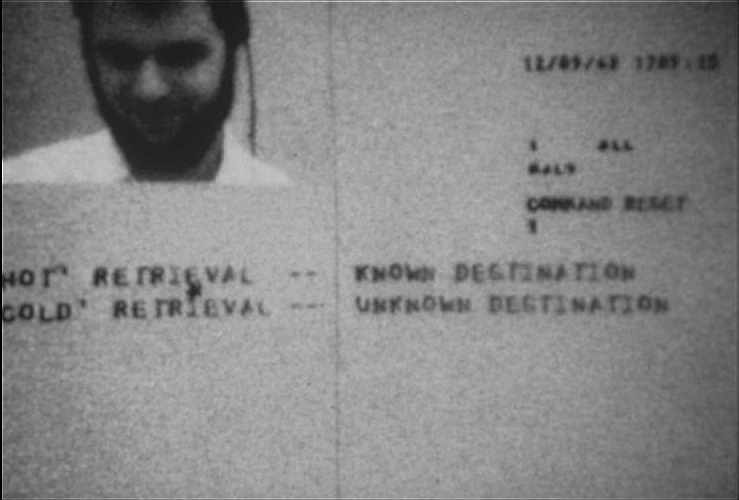
\includegraphics[width=0.5\textwidth]{images/first-videoconference}
\caption{Videoconferencing system in 1968. (source \cite{WIKI-HistoryOfVideoconferencing})}
\label{fig:FirstVideoconference1968}
\end{figure}

Nowadays, we are still used to the so-called \emph{desktop-to-desktop} communication paradigm: text messages exchanged through chat applications such as IRC, ICQ or Jabber, sound and image transmission using applications such as Skype or MS NetMeeting, which even allow for a limited multi-user videoconferences. There are, however, cases when these services simply do not suffice, when whole groups become participants in a session -- we call this the \emph{group-to-group} communication paradigm. The differences is immediately reflected to the increased hardware and software demands.
Each group usually utilizes multiple cameras and other visualization aids.
Especially the sound quality plays a dominant role in the conference rooms.
When groups are involved, the amount of intrusive effects such as echo rises significantly.

However, the usefulness of the technology is always limited by the simplicity, availability and affordability of the particular technology, regardless of the audience involved (groups of scientists, team members within a company, teachers and students).

Scientific workplaces and universities have always been connected to the fastest networks available to on market which led to the idea of utilizing the existing infrastructure for video-conferencing purposes. As an example could be the Masaryk University in Brno, where the video-conferencing node called AccessGrid Point was set up. Details can be found in the paper \cite{ArticleUVTMU-KomunikaceAGPoint}, where the authors E. Hladká and P. Holub refer to the possibility of extending the computational grids\footnote{Grid -- distributed system providing facilities to solve computationally complex problems using parallel algorithms such as physics of high energies, astrophysics and biology.} using devices enabling virtual meetings (video/conferences). Such principle has also been popular among founders of various grid-like projects, thus along with the grid infrastructure, also the AccessGrid network, composed of special videoconferencing rooms, facilitating distant high-quality collaboration, has been developed.

Within the text of this thesis, I would like to highlight alternative open-source solution as a counterpart to the expensive commercial applications available to date.
The main problem, however, is the simplicity of installation and management of such a heterogeneous and complex system. It is often easier for users to buy an expensive all-in-one solution than to adapt open-source applications.

\paragraph*{Main goals:}

\begin{enumerate}
%-------------------
\item To find a pure open-source-based solution providing video-conferencing capabilities for a group-to-group communication.
The system should run inside a UNIX-like environment, preferably on the Linux platform.

%-------------------
\item To implement session recording, editing and archiving.
\end{enumerate}

The central technology in this work is the AccessGrid project.
We are going to compare it to the other existing technologies, to discuss its advantages and drawbacks and to describe ideas and further improvements of the platform. As a proof-of-concept we built a real video-conference room which demonstrates the feasibility of our approach and hopefully brings the AccessGrid technology closer to ordinary users.
		
%%%%%%%%%%%%%%%%%%%%%%%%%%%%%%%%%%%%%%%%%%%%%%%%%%%%%%%%%%%%%%%%%%%%%
%%%%%%%%%%%%%%%%%%%%%%%%%%%%%%%%%%%%%%%%%%%%%%%%%%%%%%%%%%%%%%%%%%%%%
%%%%%%%%%%%%%%%%%%%%%%%%%%%%%%%%%%%%%%%%%%%%%%%%%%%%%%%%%%%%%%%%%%%%%
%%%%%%%%%%%%%%%%%%%%%%%%%%%%%%%%%%%%%%%%%%%%%%%%%%%%%%%%%%%%%%%%%%%%%
\chapter{Choosing the technology}\label{kap:VyberTechnologie}
%%%%%%%%%%%%%%%%%%%%%%%%%%%%%%%%%%%%%%%%%%%%%%%%%%%%%%%%%%%%%%%%%%%%%
%%%%%%%%%%%%%%%%%%%%%%%%%%%%%%%%%%%%%%%%%%%%%%%%%%%%%%%%%%%%%%%%%%%%%
%%%%%%%%%%%%%%%%%%%%%%%%%%%%%%%%%%%%%%%%%%%%%%%%%%%%%%%%%%%%%%%%%%%%%
%%%%%%%%%%%%%%%%%%%%%%%%%%%%%%%%%%%%%%%%%%%%%%%%%%%%%%%%%%%%%%%%%%%%%

%%%%%%%%%%%%%%%%%%%%%%%%%%%%%%%%%%%%%%%%%%%%%%%%%%%%%%%%%%%%%%%%%%%%%
%%%%%%%%%%%%%%%%%%%%%%%%%%%%%%%%%%%%%%%%%%%%%%%%%%%%%%%%%%%%%%%%%%%%%
\section{Motivation}
%%%%%%%%%%%%%%%%%%%%%%%%%%%%%%%%%%%%%%%%%%%%%%%%%%%%%%%%%%%%%%%%%%%%%
%%%%%%%%%%%%%%%%%%%%%%%%%%%%%%%%%%%%%%%%%%%%%%%%%%%%%%%%%%%%%%%%%%%%%

One of the goals of this work is the utilization of open-source components.
We are going to combine several components and thus requiring access to their source code.
Many proprietary systems tend to push their proprietary protocols which hinders users from customization.

Some of the open standards concerning our effort are defined by the IETF\index{IETF}\footnote{Internet Engineering Task Force} organization which also defines important Internet standards. The standardization process within IETF is public in a form of RFC\index{RFC}\footnote{Request For Comments} documents which are collaboratively being developed by experts and the community. For the purposes of our thesis, we can use RFC as a source of standards for sound and video transmissions using the IP protocol.

Despite what we already said about proprietary systems, we could get inspired from the user experience and ergonomy of use point of view. Moreover, products such as VRVS \cite{VRVS-SK-Manual} or InSORS have already been founded on the infrastructure of existing open-source components (in this case the MBone tools). We could therefore easily reuse their approach in certain situations.

Last but not least, as stated in \cite{OpenMashProject}, we should be aware of the fact that the requirements of the scientific community will differ from the requirements of the commercial sector, some even being in conflict.

The rest of this chapter discusses the features of selected applications. The selection is based on personal preference of the author.

%%%%%%%%%%%%%%%%%%%%%%%%%%%%%%%%%%%%%%%%%%%%%%%%%%%%%%%%%%%%%%%%%%%%%%%%
%%%%%%%%%%%%%%%%%%%%%%%%%%%%%%%%%%%%%%%%%%%%%%%%%%%%%%%%%%%%%%%%%%%%%%%%
\section{Selected proprietary systems}
%%%%%%%%%%%%%%%%%%%%%%%%%%%%%%%%%%%%%%%%%%%%%%%%%%%%%%%%%%%%%%%%%%%%%%%%
%%%%%%%%%%%%%%%%%%%%%%%%%%%%%%%%%%%%%%%%%%%%%%%%%%%%%%%%%%%%%%%%%%%%%%%%

% ==================================
\subsection{Skype}\label{kap:Skype}
% ==================================
\begin{figure}
\centering
\includesvg[width=1\textwidth]{skype-architecture}
\caption{Overview of the Skype architecture.}
\label{fig:Skype-Architecture}
\end{figure}

Systém Skype sme vybrali ako zástupcu komerčne úspešného a masovo používaného systému s jednoduchou inštaláciou a obsluhou.

Obrázok \ref{fig:Skype-Architecture} znázorňuje spôsob komunikácie medzi uzlami v sieti Skype. Uzly umiestnené za sieťovým firewallom komunikujú s okolitým svetom prostredníctvom tzv. superuzlov\footnote{V ďalšom texte uvidíme ešte iné prístupy k riešeniu problémov spojených s firewallmi}. Prihlasovanie do siete sa uskutočňuje pomocou login servera. Po úspešnej autentifikácii sprostredkujú superuzly multimediálny prenos medzi koncovými klientmi. Nadväzovanie spojenia prebieha tak, že klient postupne kontaktuje najbližšie superuzly, ktoré rekurzívne kontaktujú svojich susedov až pokiaľ nie je známa trasa k volanému klientovi. Výsledné smerovanie multimediálnych paketov je zabezpečené na aplikačnej úrovni (podľa modelu ISO/OSI) a využíva sa decentralizovaná povaha siete Skype.

Spomínaná závislosť na superuzloch je priamo spojená s uzavretosťou protokolu Skype. Ako vidíme na obrázku \ref{fig:Skype-Architecture}, klient, ktorý disponuje dostatočne rýchlym pripojením a vlastnou IP adresou, sa mení na tzv. superuzol. Ako uvádza zdroj \cite{ArticleUreliable-Root-10-duvodu-proc-nepouzivat-skype}, pokiaľ by existovali alternatívne rozhrania, mohli by takéto aplikácie zabraňovať vzniku superuzlov, čo by sa následne odrazilo na celkovej kvalite prenosu v celej sieti Skype. Autori preto nemajú záujem na zverejňovaní svojho protokolu.

Automatický vznik superuzlov vedie k využívaniu prenosovej kapacity bez vedomia vlastníka siete. Problém sa prejaví pri spoplatnenom objeme prenesených dát, v Českej Republike napr. v sieti rozvodov káblovej televízie a internetu UPC alebo s pripojením ADSL.

\subsubsection*{Výhody}
\begin{paklist}
\item Jednoduchá inštalácia a obsluha.
\item Distribuovaná povaha aplikácie umožňuje prekonať NAT/firewall\index{NAT!traversal} pomocou siete superuzlov (obrázok \ref{fig:Skype-Architecture}).
\item Aplikácia je v súčasnosti zdarma, poskytovateľ umožňuje aj telefonické hovory do komerčných sietí.
\item Aplikácia je k dispozícii pre platformy Windows, Mac, Linux a Pocket PC.
\item Možnosť uskutočniť videokonferencie pomocou ďalších modulov -- text, audio, video, selektívne zdieľanie pracovnej plochy.
\item Komunikácia medzi uzlami je šifrovaná. Výmena kľúčov je zabezpečná pomocou 2048-bit RSA šifry a samotný prenos využíva 256-bit AES.
\end{paklist}

\subsubsection*{Neýhody}
\begin{paklist}
\item Uzavretý protokol.
\item Rozhranie pre platformu Linux zatiaľ vo verzii 1.3.0.53 neumožňuje prenos obrazu.
\item Vznik superuzlov, využívanie prenosovej kapacity bez vedomia vlastníka siete.
\item Aplikácia neumožňuje ovplyvňovať kvalitu prenosu priamo, nastavenie prebieha automaticky.
\item Systém nie je možné používať bez internetového pripojenia (napr. v izolovanej sieti LAN). Vždy je nutné kontaktovať Login server (obrázok \ref{fig:Skype-Architecture}).
\end{paklist}

% ==================================================
\subsection{Adobe Flash}\label{kap:Adobe Flash}
% ==================================================
Technológia Flash vzhľadom na svoje rozšírenie vo väčšine súčasných internetových prehliadačov môže ponúknuť spôsob ako dopraviť videokonferenčné riešenie k užívateľovi bez nutnosti inštalácie. Najnovšia verzia Flash 9 je dostupná pre platformy Windows, Mac a Linux, staršie verzie existujú pre platformy Solaris, HP-UX, BeOS a ďalšie. Ako príklad videokonferenčných riešení postavených na tejto technológii môžeme uviesť
InstantPresenter \cite{Company-Flash-InstantPresenter} alebo
FlashMeeting \cite{Company-Flash-FlashMeeting}.

\begin{figure}[htp]
\centering
\includesvg[width=0.6\textwidth]{flash-architecture}
%\includegraphics[width=0.45\textwidth]{images/app-flashmeeting-testtool}
%\includegraphics[width=0.45\textwidth]{images/app-flashmeeting-vote}
\caption{Architektúra Flash Media Server.}
\label{fig:Flash-Architecture}
\end{figure}

Na obrázku \ref{fig:Flash-Architecture} je znázornená centralizovaná povaha systému. Predpokladá sa, že centrálny prvok Flash Media Server disponuje verejnou IP adresou, a dostatočne rýchlym pripojením aby zvládla spracovať komunikáciu pripojených klientov (na obrázku označených ako "node"). Takto centralizovaná architektúra umožňuje prekonávať NAT/firewall\index{NAT!traversal}, pretože dokáže v krajnom prípade zabaliť komunikáciu do~TCP paketov.

Prenos multimediálnych paketov zabezpečuje proprietárny Real Time Messaging Protocol (RTMP\footnote{Nezamieňať s Routing Table Maintenance Protocolom z rodiny AppleTalk.}). Pretože neexistuje voľne dostupná špecifikácia RTMP, vznikol open-source projekt Red5 \cite{OpenSourceFlash-Red5}, ktorý pomocou reverse engineeringu\footnote{Autori označujú tento akt ako "discovery through observation".} implementuje jeho podstatnú časť \cite{OpenSourceFlash-RTMP-AMF}.
Protokol RTMP využíva UDP port 1935 a v prípade blokovania tunel cez TCP port 80 (HTTP).

\subsubsection*{Výhody}
\begin{paklist}
\item Technológia dostupná pre rôzne platformy.
\item Pokiaľ odhliadneme od nutnosti inštalovať samotný internetový prehliadač a flash-plugin, nevyžadujú ďalšie aplikácie žiadnu inštaláciu. Komunikácia prebieha priamo z internetového prehliadača.
\item Jednoduché nastavenie a kalibrácia kamery a mikrofónu.
\item Ďalšie vlastnosti, ktoré uvádza výrobca, ako napr. komunikácia cez SSL, vyvažovanie záťaže, QoS.
\item Množstvo open-source projektov súvisiacich s technológiou flash \cite{OpenSourceFlash-AllProjects}.
\end{paklist}

\subsubsection*{Neýhody}
\begin{paklist}
\item Systém je určený pre relatívne malé konferencie vzhľadom na vyššie hardwarové nároky samotnéhu flash-pluginu v porovnaní napr. s VRVS alebo AccessGridom popisovaných neskôr v tomto texte.
\item Zatiaľ neexistuje plnohodnotná open-source implementácia ani iná natívna implementácia pre architektúry x86-64, PowerPC, ARM.
\item Závislosť na reverse engineeringu.
\end{paklist}

% ==================================
\subsection{InSORS}\label{kap:InSORS}
% ==================================
Riešenie InSORS IG2 je postavené na technológii MBone o ktorej budeme hovoriť v ďalších kapitolách v súvislosti s AccessGridom (kapitola  \ref{kap:AccessGrid}). InSORS prináša integrované prostredie, ktoré zahŕňa softwarové aj hardwarové komponenty. Zákazník tak môže získať vyladený videokonferenčný systém, ktorý je ale zatiaľ dostupný iba pre platformu Windows.

\begin{figure}[htp]
\centering
\includesvg[width=0.8\textwidth]{arch-multicast}
\caption{Architektúra systému s použitím multicastovej siete.}
\label{fig:ArchMulticast}
\end{figure}

Podobne ako v prípade AccessGridu, prebieha komunikácia buď prostredníctvom multicastovej siete, alebo pomocou premostení z unicastovej siete (obrázok \ref{fig:ArchMulticast}).

Systém disponuje nástrojom IG Recorder, ktorý umožňuje okrem zvuku a obrazu nahrávať zdieľané prezentácie. Záznamy z konferencií je možné zároveň prehrať v~prebiehajúcej videokonferencií.

\subsubsection*{Výhody}
\begin{paklist}
\item Nahrávanie zdieľaných konferencií a prezentácií.
\item Integrované prostredie -- možnosť zakúpiť zároveň software aj hardware.
\item Integrácia s ostatnými VoIP technológiami, premostenie systémov H.323 a AccessGrid.
\item InSORS využíva otvorené štandardy ako napr. kodeky
H.261, H.263, H.264 (kapitoly \ref{kap:H.261}, \ref{kap:H.263}, \ref{kap:H.264}). Prenos multimediálnych dát je riešený pomocou protokolu RTP (kapitola \ref{kap:RTP+RTCP}).
\end{paklist}

\subsubsection*{Neýhody}
\begin{paklist}
\item Aplikácia je k dispozícii jedine pre platformu Windows.
\item Videokonferencia pomocou InSORS je spoplatnená.
\end{paklist}

% ==================================
\subsection{VRVS + EVO}\label{kap:VRVS}\index{VRVS!system}
% ==================================
Posledným zástupcom komerčných videokonferenčných riešení, ktorý v tejto práci popíšeme, je Virtual Rooms Videoconferencing Systems (VRVS) a jeho následník EVO. VRVS je distribuovaný systém určený pre komunikáciu v reálnom čase prístupný cez webové užívateľské rozhranie, ktoré využíva platformovo závislé aplikácie na strane klienta. Ide o upravené verzie MBone nástrojov akými sú napr. VIC (kapitola \ref{kap:VIC}) a RAT (kapitola \ref{kap:RAT}) z projektu OpenMash (kapitola \ref{kap:OpenMash}). Ďalšie komponenty, ako napr. premostenia pre softwarové alebo hardwarové H.323 klienty, používajú technológiu Java.

\begin{figure}[htp]
\centering
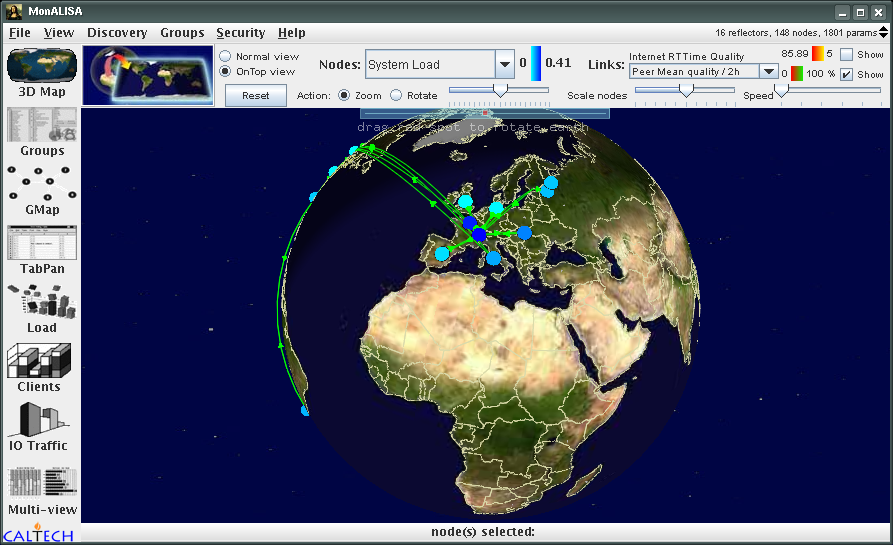
\includegraphics[width=0.48\textwidth]{images/app-monalisa1.png}
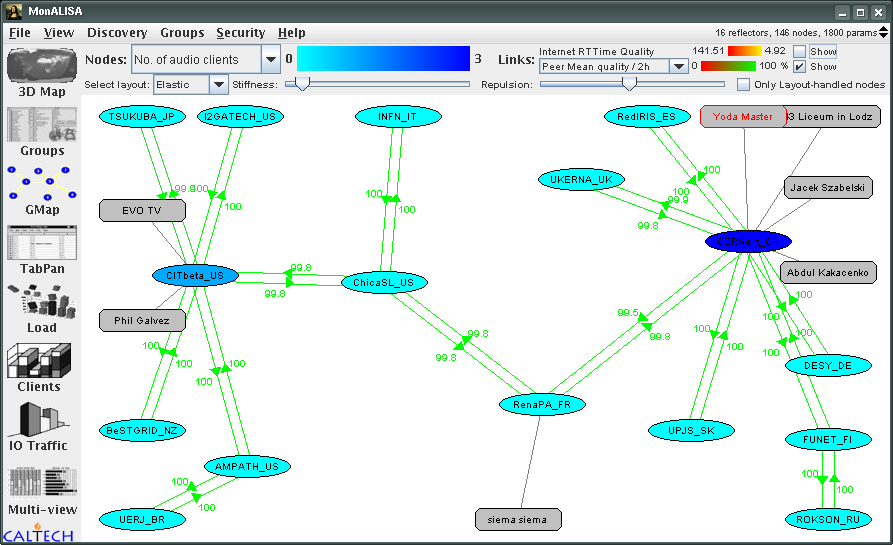
\includegraphics[width=0.48\textwidth]{images/app-monalisa3.png}
\caption{Monitorovanie distribuovaného systému VRVS reflektorov\index{VRVS!reflektor} pomocou aplikácie MonaLisa.}
\label{fig:MonaLisa-frontend}
\end{figure}

VRVS disponuje sieťou reflektorov\index{VRVS!reflektor} -- serverov rozmiestnených na rôznych miestach sveta, ktoré sprostredkovávajú komunikáciu medzi VRVS klientmi. Špeciálnym prípadom takéhoto reflektoru je VRVS-AG Reflector, ktorý umožňuje komunikovať s uzlami AccessGridu. Nezáleží, či klient disponuje unicast alebo multicast pripojením, VRVS transparentne premosťuje technológie AccessGrid, QuickTime a H.323.

Monitorovanie stavu VRVS\index{VRVS!monitoring} siete umožňuje upravená verzia systému MonaLisa\footnote{Moitoring Agents using a Large Integrated Services Architecture}. Jeho grafické rozhranie vidíme na obrázku \ref{fig:MonaLisa-frontend}. Vľavo je na svetovej mape znázornená sieť reflektorov umiestnených v Európe, vpravo je tá istá sieť znázornená vo~forme prehľadného grafu.

Zaujímavou funkciou, ktorá minimalizuje nároky na prenosovú kapacitu, je funkcia "Voice Switched mode". Autori VRVSV uvádzajú v publikácii \cite{VRVS-SK-Manual} nasledujúci príklad:

\begin{quote}
Príklad: Garantovaná kapacita siete je 1024Kbit/s. Videokonferencie sa zúčastňuje 15 partnerov. Každý vysiela kvalitný obraz (s datovými tokmi okolo 800Kbit/s). Kapacita siete by teda mala byť aspoň 12Mbit/s:

Počet účastníkov x 800 Kbit/s + 64Kbit/s (minimálny audio tok) =
= (15 x 800 + 64) Kbit/s = \textbf{12064Kbit/s}.

Riešenie: Použijeme „Voice Switched“ mode, takže vytvoríme požiadavku na VRVS reflektor\index{VRVS!reflektor}, aby posielal len video tok od toho partnera, ktorý práve rozpráva. Splnením tejto požiadavky dosiahneme obmedzenie toku na úroveň:

1 x 800Kbit/s (video) + 64Kbit/s (audio) = \textbf{864Kbit/s}.
\end{quote} 

Podobne ako InSORS a AccessGrid, podporuje VRVS aj nahrávanie konferencií. To však prebieha na strane servera, kde poverený operátor manuálne ovláda nahrávanie RTP paketov z vybranej virtuálnej miestnosti.

Aj keď ide o komerčný projekt California Institute of Technology, je systém dostupný zdarma pre vedeckú komunitu. Rozširovanie siete VRVS reflektorov\index{VRVS!reflektor} je spravované autormi systému. Po splnení kritérií môže záujemca poskytovať svoj vlastný reflektor pripojený do VRVS siete.
Užívatelia sú združení do skupín podľa oblasti záujmu, tzv. VRVS komunity (Internet2, SLOVAKIA\ldots)

V septembri 2003, bola otvorená Slovenská akademická videokonferenčná sieť, ktorá je k dispozícií všetkým univerzitám, výskumným ústavom SAV a vládnym organizáciám pripojených na optickú sieť SANET (Association of users of Slovak Academic data NETwork). Vznikol tak priestor pre experimentálne projekty ako napr. otvorené alebo dištančné vzdelávanie.

Nasledovníkom VRVS sa má v blízkej budúcnosti stať aplikácia EVO. Rozhranie je vytvorené v Jave a oproti VRVS podporuje navyše: Instant Messaging, Private Meetings (videokonferencia bez virtuálnej miestnosti), kryptovanie textových správ, výmenu súborov atď. Aplikácia je tiež multiplatformná.

\begin{samepage}
\subsubsection*{Výhody}
\begin{paklist}
\item Dostupnosť priamo z webového rozhrania -- automatická inštalácia.
\item Integrovaný systém rezervácie virtuálnych miestností.
\item P2P-sieť reflektorov.
\item Premostenie rozdielnych technológií.
\item Monitorovanie stavu siete.
\item Voice Switched mode.
\end{paklist}
\end{samepage}

\subsubsection*{Neýhody}
\begin{paklist}
\item Nutná výstavba siete reflektorov.
\item Užívateľ musí inštalovať Javu, potvrdzovať certifikáty.
\end{paklist}


%%%%%%%%%%%%%%%%%%%%%%%%%%%%%%%%%%%%%%%%%%%%%%%%%%%%%%%%%%%%%%%%%%%%%%%%%
%%%%%%%%%%%%%%%%%%%%%%%%%%%%%%%%%%%%%%%%%%%%%%%%%%%%%%%%%%%%%%%%%%%%%%%%%
\section{Vybrané voľne dostupné systémy}
%%%%%%%%%%%%%%%%%%%%%%%%%%%%%%%%%%%%%%%%%%%%%%%%%%%%%%%%%%%%%%%%%%%%%%%%%
%%%%%%%%%%%%%%%%%%%%%%%%%%%%%%%%%%%%%%%%%%%%%%%%%%%%%%%%%%%%%%%%%%%%%%%%%

% ================================================================
\subsection{VoIP riešenia}\label{kap:VoIP-Software}
% ================================================================
Z tejto kategórie vyberieme nasledujúce aplikácie: \textbf{Linphone}, \textbf{Ekiga}, \textbf{Wengophone} a \textbf{Asterisk}. Všetky existujú pre plaformy Windows aj Linux, sú dostupné pod licenciou GPL\footnote{General Public License $\Rightarrow$ open-source}, podporujú protokol SIP, prípadne H.323 (kapitola \ref{kap:VoIP-Protocols}).

Aplikácia Linphone umožňuje iba prenos zvuku. Ekiga a Wengophone využívajú pripojenú webkameru na prenos obrazu. Navyše poskytujú pre nových užívateľov bezplatný SIP účet \url{username@ekiga.net} resp. \url{username@voip.wengo.fr}. Wengophone dokonca poskytuje kredit pre volanie do pevnej a mobilnej telefónnej siete, prípadne prepája hovory priamo na SIP účet. Podporuje aj posielanie SMS správ.

Prenos obrazu je v oboch aplikáciách vo veľkosti CIF (obrázok \ref{fig:Resolutions}), každý uzol môže odosielať iba jeden obrazový a jeden zvukový dátový tok, čo znevýhodňuje nasadenie týchto aplikácií pre účely rozsiahlej videokonferencie, naopak postačuje pre účely desktop-to-desktop komunikácie.

Okrem SIP a H.323 klientov by sme radi spomenuli software určený pre chod telefónej ústredne (PBX). Asterisk podporuje prenos zvuku pomocou niekoľkých protoklov (IAX2, SIP, H.323), voicemail, adresárové služby, konferenčné hovory, odkazovač, prijímanie spojení čakajúcich vo fronte a ďalšie \ldots. Design protokolu IAX2 umožňuje prekonávať problémy s NAT/firewallmi\index{NAT!traversal}. Protokol SIP tiež podporuje preposielanie multimediálnych paketov cez tzv. STUN proxy server (napr. stun.ekiga.net). Nie je však natoľko úspešný ako práve IAX2.

\subsubsection*{Výhody}
\begin{paklist}
\item Existencia pre rôzne platformy, open-source, SIP je IETF štandard. IAX2 je vo fáze návrhu (IETF Internet-Draft \cite{IETFDraft-IAX2}).
\item Jednoduchá inštalácia a používanie.
\item Design IAX2 a STUN server pre SIP riešia problémy s NAT/firewallom.
\item Integrácia s telefónnymi linkami.
\item Kvalitné a efektívne kodeky ako napr. Speex.
\item Vstavané odstaňovanie spätnej väzby.
\item Pre Asterisk existuje špeciálna distribúcia Linuxu, dokonca aj vo formáte VMWare appliance.
\end{paklist}

\subsubsection*{Neýhody}
\begin{paklist}
\item Riešenia primárne určené pre telefonovanie.
\item Fixná veľkosť obrazu CIF a fixný počet dátových tokov obmedzuje použitie na desktop-to-desktop komunikáciu. Je to však problém konkrétnej implementácie, nie architektúry.
\item Kombinácia rôznych SIP klientov častokrát vedie k chybám pri spojovaní a komunikácii -- voľba nesprávneho kodeku, rozdielne implementácie protokolov.
\end{paklist}


% ============================================
\subsection{AccessGrid}\label{kap:AccessGrid}
% ============================================

Cieľom projektu AccessGrid (AG) je umožniť čo najprirodzenejšiu interakciu medzi účastníkmi konferencie s využitím existujúcej sieťovej infraštruktúry. Tento robustný nástoj pozostáva zo sady softwarových a hardwarových komponentov škálovateľných na mieru potrebám videokonferencie, od komunikácie medzi jednotlivcami až po celé skupiny.

Po softwarovej stránke tu môžeme nájsť komponenty určené na prenos obrazu, zvuku, zdieľanie prezentácií, vizualizačné a riadiace programy. Pre konferenciu prostredníctvom AG je obvykle vyhradená špeciálna miestnosť, čo umožňuje zabezpečiť kvalitnú komunikáciu aj pri veľkom počte účastníkov. Technológia AG je priamo navrhnutá pre spoluprácu medzi skupinami vedcov, kde prezentácia a vizualizácia výsledkov výskumu vyžaduje viac projekčnej techniky, kamier, náročnejšie spracovánie zvuku, a teda aj väčšie množstvo výpočtovej techniky potrebnej pre kódovanie zvuku a obrazu.

Obvykle takúto miestnosť označujeme ako uzol AccessGridu (AG node). Obrázok \ref{fig:ArchAccessGridDefault} znázorňuje príklad typickej architektúry AG node. Hneď na prvý pohľad si môžeme všimnúť distribuovanú povahu celého systému. Na obrázku sú znázornené štyri oddelené počítače -- Display Computer, Video Capture Computer, Audio Capture Computer a Control Computer. Po softwarovej stránke je AG zložený z komponentov VenueServer, VenueClient, NodeManager, NodeService a Bridge. Venue server predstavuje virtuálnu miestosť, v ktorej sa nachádzajú účastníci konferencie. Obsahuje súbory určené pre stiahnutie zdieľanými aplikáciami. Na VenueServer sa klienti pripájajú pomocou svojich VenueClientov, kde sa každý účastník autentifikuje pomocou certifikátu\footnote{O certifikát musí účastník dopredu požiadať certifikačnú autoritu. K tomuto účelu slúži špeciálny nástroj pomenovaný "Certificate Request Tool". V prípade nutnosti je možné použiť anonymný certifikát.}. NodeManager umožňuje ovládať distribuované prvky systému, zapínať a vypínať streamovacie služby. To sa deje prostredníctvom NodeService -- služieb spájajúcich oddelený hardware do distribuovaného systému, ktorý komunikuje pomocou XML-RPC. Posledným komponentom je Bridge, ktorý je určený na spostredkovanie služby pre účastnikov bez multicastovej siete.

V porovnaní s ostatnými technológiami sa môže zdať AG ako príliš zložitý systém. Kvalitný zážitok z videokonferencie za účasti veľkého počtu osôb, však vyžaduje viac investícií do zariadenia miestnosti. Obraz je na~rozdiel od monitoru zobrazovaný na projekčné plátno niekoľkými projektormi.

\begin{figure}
\centering
\includesvg[width=0.95\textwidth]{arch-ag-default}
\caption{Typická architektúra AccessGridu. (zdroje \protect\cite{ArticleUVTMU-KomunikaceAGPoint}\cite{childers00})}
\label{fig:ArchAccessGridDefault}
\end{figure}

\subsubsection*{Výhody}
\begin{paklist}
\item Škálovateľné riešenie podľa veľkosti konferencie.
\item Množstvo zdieľaných aplikácií a iných nástrojov.
\item Vysoká kvalita obrazu a zvuku.
\item Možnosť prenosu prostredníctvom unicast aj multicast siete.
\item Multiplatformnosť: Linux, Windows, MacOS X, FreeBSD
\end{paklist}

\subsubsection*{Neýhody}
\begin{paklist}
\item Architektúra vyžaduje rýchle sieťové pripojenie.
\item Bežný užívateľ môže mať problémy pri inštalácii a nastavení AG.
\item Vyššie nároky na priestor a vyššie finančné náklady na nákup potrebného hardware.
\item Problémy s multicastovým pripojením.
\item Problémy s prekonávaním NAT\index{NAT!problem}.
\end{paklist}


%%%%%%%%%%%%%%%%%%%%%%%%%%%%%%%%%%%%%%%%%%%%%%%%%%%%%%%%%%%%%%%%%%%%%%%%%
%%%%%%%%%%%%%%%%%%%%%%%%%%%%%%%%%%%%%%%%%%%%%%%%%%%%%%%%%%%%%%%%%%%%%%%%%
\section{Požiadavky a parametre zvoleného riešenia}
%%%%%%%%%%%%%%%%%%%%%%%%%%%%%%%%%%%%%%%%%%%%%%%%%%%%%%%%%%%%%%%%%%%%%%%%%
%%%%%%%%%%%%%%%%%%%%%%%%%%%%%%%%%%%%%%%%%%%%%%%%%%%%%%%%%%%%%%%%%%%%%%%%%

Predchádzajúci výber aplikácií nebol náhodný. Z komerčných riešení sme vybrali Skype pre jeho masové rozšírenie v oblasti IP telefonie a jeho schopnosť prekonávať NAT/firewall\index{NAT!traversal} pomocou distribuovaného systému superuzlov.
Adobe Flash sme vybrali pre jeho dostupnosť vo väčšine internetových prehliadačov a jednoduchosť inštalácie.
InSORS nás oslovil spôsobom, ktorým využíva technológiu MBone a ďalšie otvorené štandardy, ktoré ponúka v ľahko ovládateľnom balíku s možnosťou zakúpenia spolu so špecializovaným hardwarom.
Systém VRVS je pre nás príkladom aplikácie spustiteľnej priamo z webu (teda bez nutnosti inštalácie) a príkladom distribuovanej siete reflektorov monitorovaných systémom MonaLisa (obrázok \ref{fig:MonaLisa-frontend}).
Z~nekomerčných aplikácií sme vybrali Wengophone a Ekigu ako zástupcov SIP a H.323 a AccessGrid ako zástupcu robustného open-source videokonferenčného riešenia.

Cieľom nasledujúceho textu je definovať zoznam požiadaviek, ktoré kladieme na~výsledný systém na základe skúseností z existujúcich videokonferencčných riešení. V skutočnosti nemusí existovať systém, ktorý by vyhovoval všetkým požiadavkom, stačí ak sa tomuto ideálu priblíži.

%====================================
\subsection{Základné požiadavky}
%====================================

%---------------------
\paragraph*{Škálovateľnosť:}
Architektúra videokonferenčného systému by mala byť dostatočne flexibilná na to, aby umožňovala zároveň komunikáciu medzi veľkým aj malým počtom účastníkov, tým sa otvoria možnosti nasadenia v organizáciách nezávisle na~ich veľkosti. Veľké organizácie budú mať možnosť nasadiť distribuovanú verziu systému, zatiaľ čo malé organizácie vystačia so základným nastavaním. Príliš zaťažený systém by mal byť jednoducho rozšíriteľný o nové hardwarové komponenty. Túto myšlienku by sme mohli rozvinúť až tak ďaleko, že budeme uvažovať o~vytvorení virtuálnej univerzity s množstvom simultánne prebiehajúcich prednášok.

%---------------------
\paragraph*{Bezpečnosť:}
Umožniť šifrovanú komunikáciu v~rámci konferencie. V ideálnom prípade úplné šifrovanie všetkých správ. Možnosť voľby miery zabezpečenia. Ďalšou funkčnosťou môže byť autentifikácia a autorizácia účastníkov tak, aby mali prístup do vybranej podmnožiny prebiehajúcich konferencií. V prípade bezpečnosti budeme taktiež požadovať, aby dátové prenosy nemohli byť modifikované neznámimi subjektmi (integrita).
Pre niektoré organizácie býva práve táto požiadavka kľúčová.

%---------------------
\paragraph*{Dostupnosť:}
Hlavne vyriešenie problémov spojených s firewallmi, NAT\index{NAT!požiadavka dostupnosti} a proxy servermi. Množstvo klientov sa nachádza za istou formou NAT kvôli problémom adresovania v IPv4 sieti. Sieť býva navyše obohatená o firewall, prípadne rôzne formy tzv. transparent proxy. Dokonalý prechod cez všetky sieťové prekážky by bol veľmi komplikovaný, ale systém by mal počítať aspoň s najbežnejšími problémami, hlavne NAT.

%---------------------
\paragraph*{Modifikovateľnosť:}
Možnosť zmeny komponentov systému.

%---------------------
\paragraph*{Stabilita:}
Stabilita v čase. Systém by mal byť schopný bežať nepretržite bez pádu. V prípade poruchy by mal zanechať konzistentnú množinu dát.

%---------------------
\paragraph*{Prenosová kapacita:}
Úspech videokonferencie výrazne závisí na rýchlosti siete, ktorou účastníci disponujú.

%---------------------
\paragraph*{One-way Latency:}\index{latency!one-way}
Jednosmerná reakčná odozva je doba medzi odoslaním paketu na strane odosielateľa a prijatím paketu na strane príjemcu. V ďalšom texte nás bude hlavne zaujímať hodnota Round-trip Latency.

%---------------------
\paragraph*{Round-trip Latency:}\index{latency!round-trip}
Túto veličinu definujeme ako dobu medzi odoslaním požiadavku a prijatím odpovede ($\approx 2 \times one way latency$). V texte ju budeme používať pod názvom \textbf{Reakčná odozva} resp. \textbf{Latency}. V literatúre \cite{ITU-G.114-One-way-transmission-time} sa uvádza, že v~prípade zvuku by nemala presahovať 300ms, inak si účastníci rozhovoru prestávajú rozumieť. Znázorňuje to aj obrázok \ref{fig:ITU-G.114}. V prípade prenosu obrazu môže byť táto hodnota bez problémov niekoľkonásobne väčšia. V multimediálnej komunikácii preto uprednostníme nespoľahlivé nepotvrdzované doručovanie tzv. \textbf{Unreliable Unicast/Multicast}. Doručovanie pomocou UDP pred TCP.

\begin{figure}
\centering
\includesvg[width=0.7\textwidth]{mouth-to-ear-delay}
\caption{Dôsledky oneskorenia zvuku podľa ITU-T G.114 \protect\cite{ITU-G.114-One-way-transmission-time}.}
\label{fig:ITU-G.114}
\end{figure}

%---------------------
\paragraph*{Jitter:}
Rozptyl reakčnej odozvy definujeme ako zmenu reakčnej odozvy v čase. Garancia maximálnej hodnoty pre jitter umožňuje odhadnúť veľkosti bufferov. Použitie bufferov je však obmedzené celkovou latenciou.

%---------------------
\paragraph*{Hardwarové nároky:}
Zamýšľaný systém bude spracovávať desiatky nezávislých dátových tokov. Použité kodeky musia byť v tom prípade nenáročné na výpočtový výkon. Hardwarovo náročné procesy môžu zhoršiť reakčnú odozvu systému. Tento problém sa týka hlavne spracovania obrazu.

%---------------------
\paragraph*{Štandardy:}
Budeme používať štandardizované komunikačné protokoly a kodeky. Táto požiadavka plynie už z nášho zámeru požívať jedine open-source software. Pre prenos multimediálnych paketov tak prichádza do úvahy protokol RTP (kapitola \ref{kap:RTP+RTCP}).

%---------------------
\paragraph*{Dostupnosť pre rôzne platformy:}
Umožniť sledovanie konferencie minimálne na systémoch Linux a Windows.

%=======================
\subsection{Obraz}
%=======================

%---------------------
\paragraph*{Veľkost obrazu:}
Systém by mal umožniť voľbu veľkostí obrazu. Myslíme tým hlavne rozdiely medzi snímaním veľkej miestnosti s množstvom účastníkov oproti detailnému snímaniu tváre. Predpokladáme, že jednotlivé obrazové toky budeme zobrazovať na veľké projekčné plátno pomocou data-projektora, preto doporučujeme použiť aspoň formát D1 PAL 720x576 (viď obrázok \ref{fig:Resolutions}). Implicitným formátom väčšiny súčasných videokonferenčných systémov býva totiž formát CIF 352x288 resp. 352x240 (viď obrázok \ref{fig:Resolutions}). Toto obmedzenie sa týka hlavne použitého kodeku H.261 (pozri kap. \ref{kap:H.261}).

% **********************************************
% Image Resolutions
% **********************************************
\begin{figure}
\centering
\includesvg[width=0.6\textwidth]{resolutions}
\caption{Porovnanie rôznych veľkostí obrazu.}
\label{fig:Resolutions}
\end{figure}
% **********************************************

Popisované systémy Skype a Flash
(kap. \ref{kap:Skype}, \ref{kap:Adobe Flash})
pracujú s fixnou veľkosťou obrazu.
Výhodou je jednoduchšia implementácia a ovládanie zo strany užívateľa.
Naopak systémy AccessGrid, InSORS a VRVS
(kap. \ref{kap:AccessGrid}, \ref{kap:InSORS}, \ref{kap:VRVS})
dávajú možnosť voľby na úkor jednoduchosti.

%---------------------
\paragraph*{Kódovanie pohybu:}
Obraz z miestnosti, kde prebieha konferencia, može mať statickú alebo dynamickú povahu, čo by sme mali zohľadniť aj pri voľbe vhodného kodeku. Za statický obraz v tomto prípade pokladáme napr. skupinu sediacich ľudí, ktorí sú snímaní kamerou z niekoľkometrovej vzdialenosti pri konštantných svetelných podmienkach. Príkladom dynamického obrazu môže byť napr. jedna osoba snímaná z blízka, prípadne množstvo pohyblivých objektov. Slabé osvetlenie navyše spôsobuje nárast dátového toku, pretože kamery pridávajú do obrazu rôzne artefakty.

%---------------------
\paragraph*{Kvalita obrazu:}
Pokiaľ nám ide o komunikáciu medzi jednotlivcami, ktorí navyše disponujú prenosovou kapacitou menšou ako 1Mbit/s, prirodzene nám postačí nižšia kvalita obrazu ako v prípade rozsiahlej konferencie, kde obvykle vyžadujeme aspoň 10 Mbit/s. V prípade požiadavku na prenosy vo vysokej kvalite musíme počítať dokonca s kapacitou 25Mbit/s pre jeden dátový tok (komprimované video vo formáte HDV). Rozpracovanie tejto problematiky je možné nájsť napr. v článku \cite{ArticleUVTMU-VideokonferenceSVysokouKvalitou}.

%=======================
\subsection{Zvuk}
%=======================

%---------------------
\paragraph*{Kvalita zvuku:}
Na kvalitu zvuku kladieme vyššie nároky než na kvalitu obrazu. Človek je oveľa citlivejší na drobné výpadky zvuku ako na úplnú absenciu obrazu. (V~kapitole \ref{kap:RTP+RTCP}, pojednávame o protokole RTP, ktorý práve z tohto dôvodu používa oddelené UDP porty pre prenos zvuku a obrazu).
Pokiaľ chceme prenášať reč a nezaujíma nás prenos hudby v najvyššej kvalite, vystačíme s frekvenciou okolo 8000Hz. Najväčším nepriateľom pre nás bude latency (reakčná odozva) resp. jitter (rozptyl reakčnej odozvy).

%---------------------
\paragraph*{Problém spätnej väzby:}
V podmienkach ozvučenej miestnosti sa musí systém vyrovnať so vznikom spätnej väzby a inými nevhodnými zvukovými efektmi. Potlačenie ozveny má vyššiu prioritu ako samotná kvalita zvukového signálu.

%==========================================
\subsection{Prezentácia/Vizualizácia}
%==========================================

%---------------------
\paragraph*{Podporované formáty:}
Od poskytovateľa videokonferenčnej technológie sa očakáva, že bude v~maximálnej miere vychádzať v ústrety účastníkom a podporovať široké portfólio formátov. V ideálnom prípade by účastníci nemali byť obmedzovaní pri výbere formátu, ktorý chcú prezentovať. V reálnom svete však musí poskytovateľ definovať zoznam podporovaných formátov a oboznámiť s ním všetkých zainteresovaných účastníkov s dostatočným predstihom.

%---------------------
\paragraph*{Video sekvencie:}
Mali by sme podporovať rôzne kodeky a veľkosti od súborov s desiatkami MiB až po video uložené vo formáte DVD. Typickým požiadavkom užívateľa môže byť spustenie video sekvenice, ktorú je možné ovládať minimálne tlačítkom PLAY/PAUSE.

Automatické konverzie medzi video formátmi zvládajú napr. nástroje FFMPEG, MPlayer a VLC. Zvukové súbory môžeme konvertovať pomocou nástroja sox. Pre interaktívnu úpravu zvuku je vhodná aplikácia Audacity, v prípade obrazu poslúži napr. Avidemux.

%---------------------
\paragraph*{Prezentácia vo forme statických snímkov:}
Obvyklým formátom pre prípravu prezentácie bývajú formáty PDF a PPT. V~našom riešení budeme uprednostňovať formát PDF. Účastníci videokonferencie budú totiž nútení vypustiť videosekvencie a animované prechody medzi snímkami zo svojich prezentácií. Zmenší sa tak objem prenesených dát aj záťaž procesoru.

Účastníci, ktorí inklinujú k prostrediu typu Unix budú pravdepodobne používať formáty PDF, PS (PostScript) alebo ODF (Open Document Format). Užívatelia Windows prinesú pravdepodobne formáty PPT, PDF alebo ODF. Automatickú konverziu je možné zabezpečiť jednoduchým skriptom, ktorý využíva OpenOffice makrojazyk (zdroj \cite{OpenOffice-Conversion})
Ďalšie úpravy vektorových formátov pokrývajú nástroje pstoedit, a2ping a xpdf. Automatické konverzie medzi rastrovými formátmi je možné zabezpečiť pomocou balíka NetPbm a ImageMagick. Pre vizualizáciu dát pomocou skriptov môžeme využiť programy Gnuplot, R či Graphviz.

%---------------------
\paragraph*{Interaktívne 2D/3D simulácie:}
Do tejto kategórie patria rôzne 3D modely a prostredia vytvorené v špecializovaných aplikáciách typu 3D Studio Max, Blender, SolidEdge či AutoCad. Patria sem aj prostredia vytvorené pre niektorý z herných enginov ako napr. Unreal, Half-Life, Quake a mnoho ďalších. Medzi prostredia, ktoré by sme mohli podporovať patrí ďalej OpenInventor a VRML.

\begin{samepage}
\noindent
Spôsoby prezentácie by sme mohli rozdeliť do štyroch skupín:
\begin{enumerate}
\item Programy spustené na externom počítači, ktorý je pripojený S-Video signálom.
\item Programy používajúce VNC display.
\item Programy, ktoré priamo podporujú kolaboráciu.
\item Programy emulované pomocou VMWare.
\end{enumerate}
\end{samepage}

\noindent
Počas videokonferencií Polylogues sa ukázalo, že najstabilnejším riešením je použitie externého počítača pripojeného cez S-Video. Užívateľ tak môže priniesť vlastné prostredie, na ktorom má odladenú svoju prezentáciu.

%---------------------
\paragraph*{Obraz z externého zdroja:}
Už sme spomenuli, že vhodným riešením je použiť externý hardware pripojený cez S-Video do digitalizačnej karty. Nevýhodou môže byť nutnosť zakúpenia ďalšieho hardwarového komponentu. Niekedy však užívateľ nedisponuje ani S-Video výstupom, takže musíme pristúpiť napr. k inštalácii VNC.

%---------------------
\paragraph*{Kvalita:}
Pri prenose videosekvencií spolu so zvukom platia rovnaké pravidlá ako sme stanovili v požiadavkoch na obraz a zvuk. Navyše musíme brať do úvahy, že pri prezentácii snímkov, ktoré majú väčšinou statickú povahu budeme používať iné techniky, kodeky, veľkosti obrazu. Situáciu mierne komplikujú prezentácie, ktoré v~sebe obsahujú videosekvencie. Z toho dôvodu uprednostňujeme prezentáciu vo~formáte PDF.

%---------------------
\paragraph*{Ovládanie:}
Účastníci konferencie by mali dostať možnosť ovládať prebiehajúcu prezentáciu. V prípade AccessGridu je to napr. SharedPresentation alebo SharedPDF.

%=======================
\subsection{Spolupráca}
%=======================

%http://www.vide.net/cookbook/cookbook.en/
%HighlightVideoConsumer, PositionalAudioService
%http://scv.bu.edu/~putnam/ag-audio/services-2.4/doc/

Riešenie by malo podporovať rôzne formy spolupráce medzi účastníkmi konferencie. Od jednoduchého zdieľania súborov až po zdieľanú pracovnú plochu. V tomto prípade môžeme znova využiť vlastnosti VNC.

%%%%%%%%%%%%%%%%%%%%%%%%%%%%%%%%%%%%%%%%%%%%%%%%%%%%%%%%%%%%%%%%%%%%%
%%%%%%%%%%%%%%%%%%%%%%%%%%%%%%%%%%%%%%%%%%%%%%%%%%%%%%%%%%%%%%%%%%%%%
\section{Vybraný systém}
%%%%%%%%%%%%%%%%%%%%%%%%%%%%%%%%%%%%%%%%%%%%%%%%%%%%%%%%%%%%%%%%%%%%%
%%%%%%%%%%%%%%%%%%%%%%%%%%%%%%%%%%%%%%%%%%%%%%%%%%%%%%%%%%%%%%%%%%%%%

V prvej kapitole sme popísali niekoľko existujúcich aplikácií, vyberali sme hlavne prakticky odskúšané riešenia z oblasti closed-source aj open-source software. Snažili sme sa popísať technológie vhodné pre desktop-to-desktop komunikáciu ako aj pre group-to-group komunikáciu a poukázali sme na rozdiely medzi oboma prístupmi. Pre každú aplikáciu sme pripravili zoznam ich výhod a nevýhod. Vytvorili sme obraz ideálneho videokonferenčného systému tak, že sme poskytli detailný zoznam požiadaviek. To nám umožní vybrať vhodné protokoly, kodeky a komponenty. Z~voľne dostupných technológií vyberáme AccessGrid, pretože vo svete open-source sa jedná o najkomplexnejší videokonferenčný systém, ktorého základ využívajú aj niektoré komerčné produkty.

		%%%%%%%%%%%%%%%%%%%%%%%%%%%%%%%%%%%%%%%%%%%%%%%%%%%%%%%%%%%%%%%%%%%%%
%%%%%%%%%%%%%%%%%%%%%%%%%%%%%%%%%%%%%%%%%%%%%%%%%%%%%%%%%%%%%%%%%%%%%
%%%%%%%%%%%%%%%%%%%%%%%%%%%%%%%%%%%%%%%%%%%%%%%%%%%%%%%%%%%%%%%%%%%%%
%%%%%%%%%%%%%%%%%%%%%%%%%%%%%%%%%%%%%%%%%%%%%%%%%%%%%%%%%%%%%%%%%%%%%
\chapter{Protocols}
%%%%%%%%%%%%%%%%%%%%%%%%%%%%%%%%%%%%%%%%%%%%%%%%%%%%%%%%%%%%%%%%%%%%%
%%%%%%%%%%%%%%%%%%%%%%%%%%%%%%%%%%%%%%%%%%%%%%%%%%%%%%%%%%%%%%%%%%%%%
%%%%%%%%%%%%%%%%%%%%%%%%%%%%%%%%%%%%%%%%%%%%%%%%%%%%%%%%%%%%%%%%%%%%%
%%%%%%%%%%%%%%%%%%%%%%%%%%%%%%%%%%%%%%%%%%%%%%%%%%%%%%%%%%%%%%%%%%%%%

%%%%%%%%%%%%%%%%%%%%%%%%%%%%%%%%%%%%%%%%%%%%%%%%%%%%%%%%%%%%%%%%%%%%%
%%%%%%%%%%%%%%%%%%%%%%%%%%%%%%%%%%%%%%%%%%%%%%%%%%%%%%%%%%%%%%%%%%%%%
\section{Multicast}\label{kap:Multicast}
%%%%%%%%%%%%%%%%%%%%%%%%%%%%%%%%%%%%%%%%%%%%%%%%%%%%%%%%%%%%%%%%%%%%%
%%%%%%%%%%%%%%%%%%%%%%%%%%%%%%%%%%%%%%%%%%%%%%%%%%%%%%%%%%%%%%%%%%%%%

% **********************************************
\begin{figure}
\centering
\includesvg[width=1\textwidth]{unicast-multicast}
\caption{Rozdiely medzi doručovaním metódou unicast a multicast.}
\label{fig:UnicastMulticast}
\end{figure}
% **********************************************

Vzhľadom na skutočnosť, že v~rámci videokonferencie spolu komunikuje istá skupina uzlov, začneme túto kapitolu vysvetlením rozdielov medzi spôsobmi doručovania paketov v kontexte skupinovej komunikácie.
Vysvetlíme rozdiely medzi stratégiami \textbf{unicast} a \textbf{multicast}\footnote{Doručovanie formou broadcastu nás zaujímať nebude, pretože sa väčšinou obmedzuje na doručovanie v rámci jedného segmentu siete. Navyše multicast je silnejší pojem a dokáže ho efektívne emulovať.}. Z pohľadu spoľahlivosti nám pôjde o nespoľahlivé a nespojované služby, ktoré sú vhodné pre multimediálne prenosy. Zabezpečenie spoľahlivého doručovania by malo za následok nárast latencie. Rozdiel v efektivite doručovania sme schematicky znázornili na obrázku \ref{fig:UnicastMulticast}. Je dôležité si uvedomiť, že popisujeme situáciu, kedy jeden odosielateľ posiela rovnakú správu skupine príjemcov. Nielenže chceme riešiť otázku \textbf{efektivity}, ale aj otázku \textbf{adresovania skupiny} príjemcov.

\paragraph*{Unicast:} Je spôsob doručovania, kde odosielateľ musí každému príjemcovi osobitne zaslať každý paket. Je to základný spôsob doručovania v súčasnom internete, ktorý však plytvá prenosovou kapacitou siete, pretože vyžaduje duplikovanie paketov. Navyše odosielateľ musí poznať adresu každého príjemcu. Na obrázku \ref{fig:UnicastMulticast} (1) je táto situácia znázornená ako 4 dátové toky vychádzajúce od odosielateľa. 

\paragraph*{Multicast:} Je spôsob doručovania, kedy odosielateľ posiela pakety na skupinovú adresu. Pakety sú duplikované až pri prechode medzi sieťami. Multicast tak šetrí prenosovú kapacitu. Pre správne fungovanie musia všetky uzly v sieti vrátane prepínačov a smerovačov podporovať tento spôsob doručovania, čo vyžaduje úpravy v~pôvodnom unicastovom spôsobe doručovania (RFC 1112 \cite{RFC-1112-HostExtensionsForIPMulticasting}). V protokole IPv4 je pre multicast vyhradená skupina adries tzv. class D. Sú to adresy začínajúce v~binárnom zápise prefixom 1110, v protokole IPv6 prefixom 11111111. Každá adresa určuje multicastovú skupinu pre doručovanie. Členstvo v týchto skupinách riadi protokol IGMP. Skupina zariadení, ktoré podporujú protokol IGMP, tvorí v~rámci internetu virtuálnu sieť MBone (multicast backbone). Sieť je tvorená buď špecializovanými hardwarovými komponentmi, alebo počítačmi s~podporou IGMP v~operačnom systéme. Smerovanie multicastových paketov navyše vyžaduje podporu niektorého z~multicastových routovacích protokolov DVMRP (multicastová verzia RIP), MOSPF (multicastová verzia OSPF) alebo PIM (Protocol Independent Multicasting). Táto práca však o routovaní nepojednáva.

V súčasnosti je dostupnosť multicastových služieb na nízkej úrovni a pre bežných užívateľov prakticky nedostupná. Zmenu by mal priniesť prechod na protokol IPv6, ktorý obsahuje multicast ako svoju neoddeliteľnú súčasť. Každopádne, univerzity a iné vybrané inštitúcie majú k multicastu väčšinou prístup.

%%%%%%%%%%%%%%%%%%%%%%%%%%%%%%%%%%%%%%%%%%%%%%%%%%%%%%%%%%%%%%%%%%%%%
\subsection{IGMP}
%%%%%%%%%%%%%%%%%%%%%%%%%%%%%%%%%%%%%%%%%%%%%%%%%%%%%%%%%%%%%%%%%%%%%
Pre pochopenie multicastových služieb v IPv4 sieti je nutné poznať protokol IGMP -- Internet Group Management Protocol, ktorý pomáha udržovať informácie o zložení skupín na danom sieťovom segmente. Pre správne doručovanie multicastových paketov musí byť podporovaný všetkými koncovými uzlami a smerovačmi. (Smerovače môžu byť totiž členmi multicastovej skupiny).

Táto informácia je dôležitá hlavne pri nákupe potrebného hardware. Smerovače s podporou IGMP sú totiž podstatne drahšie ako ich bežné ekvivalenty. V dobe tvorby tohto textu sa cena najlacnejšieho zariadenia\footnote{Allied Telesyn AT-AR300V2SECPK} pohybovala okolo 5000 CZK bez DPH. Priemerná cena je však okolo 10000 CZK.

% **********************************************
% IGMP Packet Format.
% **********************************************
\begin{table}[htp]
\centering
\begin{tabular}[t]{|c|c|c|c|c|}
4b & 1b & 3b & 8b & 16b \\
\hline	Version & Type & Unused & Max. response time & Checksum\\
\hline	\multicolumn{5}{|c|}{Group address} \\
\hline	\multicolumn{5}{|c|}{IGMP packet structure} \\
		\multicolumn{5}{|c|}{\vdots} \\
\hline
\end{tabular}
\caption{Formát IGMP paketu.}
\label{tab:IGMP-packet-format} 
\end{table} 
% **********************************************

Multicastový smerovač na každom segmente vysiela periodické správy Memberhip Query (tab. \ref{tab:IGMP-Membership-query}), kde Group Address = 0 (tzv. General Membership Query). Uzol, ktorý je členom tejto skupiny, odpovie zaslaním správy typu Membership Report (tab. \ref{tab:IGMP-Membership-report}). Aby nedochádzalo k zahlteniu segmentu odpoveďami od všetkých uzlov v skupine, každý uzol čaká náhodne zvolený interval pred tým, než začne vysielať.

Uzol, ktorý sa prihlasuje alebo opúšťa skupinu, zasiela tzv. State Change Report, čo je modifikovaný Membership Report (tab. \ref{tab:IGMP-Membership-report}). Pri odchode uzla zo skupiny môže nastať situácia, že skupina už neobsahuje ďalšie uzly. V takom prípade by mala skupina zaniknúť. Po každom odchode nejakého uzla odošle smerovač Group Specific Membership Query (znova modifikovaná verzia Membership Query) a uzly odpovedajú znova pomocou Membership Report.

Detailný popis protokolu IGMP sa nachádza v RFC 3376 \cite{RFC-3376-IGMP-Protocol}.


% **********************************************
% IGMP Membership Query.
% **********************************************
\begin{table}[htp]
\centering
\begin{tabular}[t]{|c|c|c|c|c|}
4b & 1b & 3b & 8b & 16b \\
\hline	\multicolumn{3}{|c|}{Type = 0x11} & Max Resp Code & Checksum \\
\hline	\multicolumn{5}{|c|}{Group address} \\
\hline	Resv & S & QRV & QQIC & Number of Sources (N) \\
\hline	\multicolumn{5}{|c|}{Source Address [1]} \\
		\multicolumn{5}{|c|}{\vdots} \\
		\multicolumn{5}{|c|}{Source Address [N]} \\
\hline
\end{tabular}
\caption{IGMP Membership Query.}
\label{tab:IGMP-Membership-query} 
\end{table} 
% **********************************************


% **********************************************
% IGMP Membership Report.
% **********************************************
\begin{table}[htp]
\centering
\begin{tabular}[t]{|c|c|c|}
8b & 8b & 16b \\
\hline	Type = 0x22 & Reserved & Checksum \\
\hline	\multicolumn{2}{|c|}{Reserved} & Number of Group Records (N) \\
\hline	\multicolumn{3}{|c|}{Group Record [1]} \\
		\multicolumn{3}{|c|}{\vdots} \\
		\multicolumn{3}{|c|}{Group Record [N]} \\
\hline
\end{tabular}

\begin{center}
Group Record má nasledujúci formát:
\end{center}

\begin{tabular}[t]{|c|c|c|}
8b & 8b & 16b \\
\hline	Record Type & Aux Data Len & Number of Sources (N) \\
\hline	\multicolumn{3}{|c|}{Multicast Address} \\
\hline	\multicolumn{3}{|c|}{Source Address [1]} \\
		\multicolumn{3}{|c|}{\vdots} \\
		\multicolumn{3}{|c|}{Source Address [N]} \\
\hline	\multicolumn{3}{|c|}{Auxiliary Data} \\
\hline
\end{tabular}

\caption{IGMP Membership Report.}
\label{tab:IGMP-Membership-report}
\end{table} 
% **********************************************

%%%%%%%%%%%%%%%%%%%%%%%%%%%%%%%%%%%%%%%%%%%%%%%%%%%%%%%%%%%%%%%%%%%%%
\subsection{SAP}
%%%%%%%%%%%%%%%%%%%%%%%%%%%%%%%%%%%%%%%%%%%%%%%%%%%%%%%%%%%%%%%%%%%%%
Session Announcement Protocol (SAP), definovaný v RFC 2327 \cite{RFC-2974-SAP-Protocol}, umožňuje periodicky vysielať informácie o prebiehajúcom multimediálnom prenose na vybrané multicastové adresy. Potenciálni príjemcovia SAP paketu môžu tento popis použiť na spustenie a nastavenie potrebného dekódovacieho nástroja.

% **********************************************
% SAP Packet Format.
% **********************************************
\begin{table}[htp]
\centering
\begin{tabular}[t]{|c|c|c|c|c|c|c|c|}
3b & 1b & 1b & 1b & 1b & 1b & 8b & 16b \\
\hline	V = 1 & A & R & T & E & C & auth len & msg id hash \\
\hline	\multicolumn{8}{|c|}{} \\
		\multicolumn{8}{|c|}{originating source (32 or 128 bits)} \\
		\multicolumn{8}{|c|}{} \\
\hline	\multicolumn{8}{|c|}{optional authentication data} \\
		\multicolumn{8}{|c|}{\vdots} \\
\hline	\multicolumn{8}{|c|}{optional payload type} \\
		\cline{2-8}
		\multicolumn{1}{|r|}{\ldots} & 0 & \multicolumn{6}{|l|}{\ldots} \\
		\cline{1-2}
		\multicolumn{8}{|c|}{payload} \\
		\multicolumn{8}{|c|}{} \\
\hline
\end{tabular}
\caption{Formát SAP paketu.}
\label{tab:SAP-packet-format} 
\end{table} 
% **********************************************

\begin{quote}
Príklad: Nech existuje odosielateľ, ktorý generuje RTP pakety na multicastovú adresu 224.0.0.1. Obraz zakódovaný kodekom H.263 odosiela na port 10000, zvuk zakódovaný ako L16 na port 20000. Pre príjem obrazu a zvuku je preto nutné spustiť na strane príjemcu aplikácie VIC a RAT:

\verb|vic 224.0.0.1/10000 & rat 224.0.0.1/20000|
\end{quote}


%%%%%%%%%%%%%%%%%%%%%%%%%%%%%%%%%%%%%%%%%%%%%%%%%%%%%%%%%%%%%%%%%%%%%
\subsection{MADCAP}
%%%%%%%%%%%%%%%%%%%%%%%%%%%%%%%%%%%%%%%%%%%%%%%%%%%%%%%%%%%%%%%%%%%%%

% **********************************************
% MADCAP Packet Format
% **********************************************
\begin{table}[htp]
\centering
\begin{tabular}[t]{|c|c|c|}
8b & 8b & 16b \\
\hline	version & msgtype & addrfamily \\
\hline	\multicolumn{3}{|c|}{xid} \\
\hline	\multicolumn{3}{|c|}{Options} \\
		\multicolumn{3}{|c|}{\vdots} \\
\hline
\end{tabular}
\caption{Formát MADCAP paketu.}
\label{tab:MADCAP-packet-format} 
\end{table} 
% **********************************************

Tento protokol podobný DHCP umožňuje dynamicky alokovať multicastové adresy. Funguje ako alternatíva k statickej alokácii, kde adresy priraďuje administrátor. Podľa modelu ISO/OSI hovoríme o protokole aplikačnej vrstvy. Používa port 2535 (UDP). Klienti kontaktujú niektorý z MADCAP serverov pomocou unicastu alebo multicastu. Server odpovedá vždy pomocou unicastu. Protokoly DHCP a MADCAP sa používajú v disjunktných sférach.


%%%%%%%%%%%%%%%%%%%%%%%%%%%%%%%%%%%%%%%%%%%%%%%%%%%%%%%%%%%%%%%%%%%%%
\subsection{UMTP}\label{kap:UMTP}
%%%%%%%%%%%%%%%%%%%%%%%%%%%%%%%%%%%%%%%%%%%%%%%%%%%%%%%%%%%%%%%%%%%%%
Riešenie problémov spojených s nedostupnosťou multicastových služieb by mal riešiť protokol UMTP \cite{IETFDraft-UMTP}, ktorého štandardizácia je v stave IETF Internet-Draft. Ako ukazujú výsledky z najnovšej verzie AccessGridu 3, môžeme sa tešiť na silný nástroj, ktorý rieši problémy spojené s prechodom cez NAT a firewall. Jednou z prvých implementácií je aplikácia AGConnector, ktorej fungovanie znázorňuje obrázok \ref{fig:AGConnector}.


%%%%%%%%%%%%%%%%%%%%%%%%%%%%%%%%%%%%%%%%%%%%%%%%%%%%%%%%%%%%%%%%%%%%%
%%%%%%%%%%%%%%%%%%%%%%%%%%%%%%%%%%%%%%%%%%%%%%%%%%%%%%%%%%%%%%%%%%%%%
\section{Multimedia-related protocols}\label{kap:Multimedia}
%%%%%%%%%%%%%%%%%%%%%%%%%%%%%%%%%%%%%%%%%%%%%%%%%%%%%%%%%%%%%%%%%%%%%
%%%%%%%%%%%%%%%%%%%%%%%%%%%%%%%%%%%%%%%%%%%%%%%%%%%%%%%%%%%%%%%%%%%%%


%%%%%%%%%%%%%%%%%%%%%%%%%%%%%%%%%%%%%%%%%%%%%%%%%%%%%%%%%%%%%%%%%%%%%
\subsection{RTP and RTCP}\label{kap:RTP+RTCP}
%%%%%%%%%%%%%%%%%%%%%%%%%%%%%%%%%%%%%%%%%%%%%%%%%%%%%%%%%%%%%%%%%%%%%
RTP (Real Time Transport Protocol) je protokol navrhnutý pre prenos dát v reálnom čase. Podľa modelu ISO/OSI ide o protokol aplikačnej vrstvy. Spolu s protokolom RTCP (Real Time Control Protocol) tvorí rámec vhodný hlavne na prenos multimediálnych dát prostredníctvom unicastovej alebo multicastovej siete.

Zatiaľ čo RTP prenáša samotné dáta, RTCP umožňuje monitorovať a riadiť doručovanie RTP paketov. Protokoly neobsahujú funkcie pre rezerváciu zdrojov ani QoS (quality of service), pre ktoré je potrebná spolupráca s nižšími vrstvami\footnote{Pre rezerváciu zdrojov a QoS je možné použiť protokol RSVP popísaný v kapitole \ref{kap:RSVP}.}. Umožňujú ale identifikovať možné zmeny v sieti a prispôsobiť vlastnosti vysielača alebo prijímača napr. zmenou kodeku, kvality alebo bufferovania. Oba protokoly sú navrhnuté tak, aby boli nezávislé na použitých sieťových a transportných vrstvách.

Detailný popis oboch protokolov sa nachádza v RFC 3550 \cite{RFC-3550-RTP-Protocol}. Pre naše účely je vhodné spomenúť, že pri videokonferenčných prenosoch bude zvuk a obraz prenášaný nezávislými dátovými tokmi. Každý tok je reprezentovaný dvoma UDP portami -- obvykle port s párnym číslom $N$ pre RTP-data a port $N+1$ pre RTCP pakety. Tvorcovia protokolu vychádzali z predpokladu, že niektorí účastníci môžu požadovať iba príjem niektorých dátových tokov (napr. iba príjem zvuku z dôvodu pomalej linky). Takéto rozdelenie však v praxi spôsobuje problémy pri prechode cez NAT/firewall. Úspešnejší sa zdá byť protokol IAX2 (kapitola \ref{kap:IAX2}), ktorý prenáša všetky dáta na jednom UDP porte.

RFC 3550 popisuje aj využitie RTP mixerov, ktoré umožňujú multiplexing dátových tokov a RTP translatorov, meniacich obsah dátového toku napr. pri preklade medzi multicastovou a unicastovou sieťou.

Synchronizácia dátových tokov je zabezpečená časovými razítkami obsiahnutými v~rámci RTCP.

% **********************************************
% RTP Packet Format
% **********************************************
\begin{table}[htp]
\centering
\begin{tabular}[t]{|c|c|c|c|c|c|c|}
0b & 0b & 0b & 0b & 0b & 0b & 0b \\
\hline	V=2 & P & X & CSRC count & M & payload type & sequence number \\
\hline	\multicolumn{7}{|c|}{timestamp} \\
\hline	\multicolumn{7}{|c|}{synchronization source (SSRC) identifier} \\
\hline	\multicolumn{7}{|c|}{contributing source (CSRC) identifiers} \\
		\multicolumn{7}{|c|}{\vdots} \\
\hline
\end{tabular}
\caption{Formát RTP paketu.}
\label{tab:RTP-packet-format} 
\end{table} 
% **********************************************

Tabuľka \ref{tab:RTP-packet-format} popisuje formát RTP paketu, z ktorého sú pre nás najdôležitejšie nasledujúce položky:

\paragraph*{payload type:} Informácia o obsahu paketu, ktorá je buď implicitne definovaná v~RFC 3551 \cite{RFC-3551-RTP-Profile-AudioVideo}, alebo dohodnutá mimo RTP.

\paragraph*{sequence number:} Číslo inkrementované s každým paketom umožňuje detekciu straty paketov. Na začiatku session býva obvykle zvolená náhodná hodnota.

\paragraph*{timestamp:} časové razítko dátového toku, záleží na obsahu, umožňuje výpočet hodnoty jitter (rozptyl reakčnej odozvy). Na začiatku session je hodnota obvykle volená náhodne a inkrementovaná podľa vnútorných hodín odosielateľa.

\paragraph*{synchronization source (SSRC) identifier:} Umožňuje príjemcovi identifikovať entitu, ktorá paket odoslala.


%%%%%%%%%%%%%%%%%%%%%%%%%%%%%%%%%%%%%%%%%%%%%%%%%%%%%%%%%%%%%%%%%%%%%
\subsection{RSVP}\label{kap:RSVP}
%%%%%%%%%%%%%%%%%%%%%%%%%%%%%%%%%%%%%%%%%%%%%%%%%%%%%%%%%%%%%%%%%%%%%
Resource Reservation Protocol (RSVP) \cite{RFC-2205-RSVP-Protocol} umožňuje príjemcovi požadovať rezerváciu sieťových zdrojov počas unicastových alebo multicastových dátových prenosov. Pre správne fungovanie QoS musia všetky smerovače na ceste od zdroja k príjemcovi podporovať RSVP. Podľa modelu ISO/OSI ide o protokol transportnej vrstvy, ktorý pracuje nad IPv4 alebo IPv6. RSVP neprenáša aplikačné dáta, funguje len ako riadiaci mechanizmus. RSVP sa zaoberá iba nastavením QoS pre prenášané pakety na~rozdiel od smerovacích protokolov, ktoré rozhodujú o ceste paketov.

% **********************************************
% RSVP Packet Format
% **********************************************
\begin{table}[htp]
\centering
\begin{tabular}[t]{|c|c|c|c|}
4b & 8b & 16b & 32b \\
\hline	V=2 & flags & Message Type & RSVP Checksum \\
\hline	\multicolumn{2}{|c|}{Send TTL} & Reserved & RSVP Length \\
\hline	\multicolumn{4}{|c|}{RSVP header structure} \\
\hline
\end{tabular}
\caption{Formát RSVP paketu.}
\label{tab:RSVP-packet-format} 
\end{table} 
% **********************************************


%%%%%%%%%%%%%%%%%%%%%%%%%%%%%%%%%%%%%%%%%%%%%%%%%%%%%%%%%%%%%%%%%%%%%
\subsection{RTSP}\label{kap:RTSP}
%%%%%%%%%%%%%%%%%%%%%%%%%%%%%%%%%%%%%%%%%%%%%%%%%%%%%%%%%%%%%%%%%%%%%
Real Time Streaming Protocol (RTSP) \cite{RFC-2326-RTSP-Protocol} môžeme podľa modelu ISO/OSI zaradiť medzi protokoly aplikačnej vrstvy. Využíva sa pri streamovaní multimediálnych dát. Umožňuje prijímajúcej strane ovládať priebeh streamovania. Syntax pripomína HTTP a podporovanými metódami sú napr. PLAY, RECORD, SETUP, PAUSE atď. \ldots Protokol RTSP nie je určený na prenos dát, ten je riešený iným mechanizmom, napr. pomocou RTP. Môžeme ho nájsť implementovaný napr. v aplikácii MPlayer ako jeden z možných spôsobov prenosu multimediálneho obsahu.
\begin{quote}
Príklad: \verb|mplayer rtsp://path/to/stream|
\end{quote}


%%%%%%%%%%%%%%%%%%%%%%%%%%%%%%%%%%%%%%%%%%%%%%%%%%%%%%%%%%%%%%%%%%%%%
\subsection{SDP}\label{kap:SDP}
%%%%%%%%%%%%%%%%%%%%%%%%%%%%%%%%%%%%%%%%%%%%%%%%%%%%%%%%%%%%%%%%%%%%%
Session Description Protocol (SDP), popísaný v RFC 2327 \cite{RFC-2327-SDP-Protocol}, je vhodný na popis multimediálnych dátových tokov v unicastovej alebo multicastovej sieti. Umožňuje nastaviť parametre aplikácie, ktorá bude tieto dáta interpretovať. Podľa modelu ISO/OSI ide o protokol aplikačnej vrstvy.

\begin{quote}
Príklad: Streamovací server na adrese 239.255.42.42 má uložené prednášky, ktoré môže klient prijať vo vysokej alebo v nízkej kvalite. Každý takýto dátový tok je reprezentovaný SDP súborom.
Pre príjem môže použiť napr. aplikáciu MPlayer:
\begin{verbatim}
mplayer sdp://presentation_01_low.sdp
\end{verbatim} 

\ldots Príslušný SDP súbor môže vyzerať nasledovne:
\begin{verbatim}
v=0
o=- 49451 3 IN IP4 127.0.0.1
s=Test MPEG Audio+Video session
i=Session streamed by testMPEG1or2AudioVideoStreamer
t=0 0
a=tool:testMPEG1or2AudioVideoStreamer
a=type:broadcast
m=audio 6666 RTP/AVP 14
c=IN IP4 239.255.42.42/127
m=video 8888 RTP/AVP 32
c=IN IP4 239.255.42.42/127
\end{verbatim}
\end{quote}


%%%%%%%%%%%%%%%%%%%%%%%%%%%%%%%%%%%%%%%%%%%%%%%%%%%%%%%%%%%%%%%%%%%%%
%%%%%%%%%%%%%%%%%%%%%%%%%%%%%%%%%%%%%%%%%%%%%%%%%%%%%%%%%%%%%%%%%%%%%
\section{VoIP protocols}\label{kap:VoIP-Protocols}
%%%%%%%%%%%%%%%%%%%%%%%%%%%%%%%%%%%%%%%%%%%%%%%%%%%%%%%%%%%%%%%%%%%%%
%%%%%%%%%%%%%%%%%%%%%%%%%%%%%%%%%%%%%%%%%%%%%%%%%%%%%%%%%%%%%%%%%%%%%


%%%%%%%%%%%%%%%%%%%%%%%%%%%%%%%%%%%%%%%%%%%%%%%%%%%%%%%%%%%%%%%%%%%%%
\subsection{SIP}
%%%%%%%%%%%%%%%%%%%%%%%%%%%%%%%%%%%%%%%%%%%%%%%%%%%%%%%%%%%%%%%%%%%%%
Session Initiation Protocol je otvorený signalizačný protokol určený pre uskutočňovanie telefónnych hovorov prostredníctvom IP siete. Jedná sa o textovo-orientovaný protkol aplikačnej vrstvy, je definovaný v RFC 3261 \cite{RFC-3261-SIP-Protocol}. Spojenie je zabezpečené prostredníctvom dvoch typov uzlov -- User Agent a Server. Spojenie môže byť naviazané aj medzi dvoma klientmi bez účasti servera. Niekoľko aplikácií, používajúcich SIP, sme popísali v kapitole \ref{kap:VoIP-Software}. Užívateľ je adresovaný pomocou URL \texttt{sip:username@hostname}. Prechod cez firewall a NAT je zabezpečený pomocou STUN servera.


%%%%%%%%%%%%%%%%%%%%%%%%%%%%%%%%%%%%%%%%%%%%%%%%%%%%%%%%%%%%%%%%%%%%%
\subsection{H.323}
%%%%%%%%%%%%%%%%%%%%%%%%%%%%%%%%%%%%%%%%%%%%%%%%%%%%%%%%%%%%%%%%%%%%%
Protokol z dieľne ITU, ktorý konkuruje protokolu SIP. Je integrovaný v niektorých hardwarových zariadeniach určených pre IP telefóniu. Túto kapitolu uvádzame iba z didaktických dôvodov, pretože na niekoľkých miestach v texte práce spomíname zariadenia podporujúce H.323. Napríklad systém VRVS disponuje premostením zo~sveta H.323.


%%%%%%%%%%%%%%%%%%%%%%%%%%%%%%%%%%%%%%%%%%%%%%%%%%%%%%%%%%%%%%%%%%%%%
\subsection{IAX2}\label{kap:IAX2}
%%%%%%%%%%%%%%%%%%%%%%%%%%%%%%%%%%%%%%%%%%%%%%%%%%%%%%%%%%%%%%%%%%%%%
Inter Asterisk Exchange je binárny protokol určený pre komunikáciu telefónnych ústrední Asterisk\footnote{Asterisk PBX uvádzame v kapitole \protect\ref{kap:VoIP-Software}} a ďalšie VoIP služby. Jeho štandardizácia je zatiaľ v štádiu IETF Internet-Draft \cite{IETFDraft-IAX2}. Podľa modelu ISO/OSI je IAX protokolom aplikačnej vrstvy. Využitie by mohol nájsť aj vo veľkých videokonferenčných systémoch akým je AccessGrid, prípadne ako protokol pre streamovanie multimediálneho obsahu. Kombinuje v~sebe vlastnosti \textbf{kontrolného}, \textbf{transportného} a \textbf{signalizačného} protokolu, takže zastupuje funkčnosť protokolov RTP/RTCP, SIP, H.323. Na prenos všetkých IAX paketov sa využíva jeden statický UDP port 4569, to mu umožňuje prekonávať problémy spojené s firewallmi a NAT. IAX nepotrebuje externý proxy server ako napríklad SIP, ani žiadne špeciálne nastavenie firewallu (okrem neblokovania portu 4569). Môžeme preto tvrdiť, že by mohol nahradiť protokoly RTP/RTCP, SIP, H.323.

%%%%%%%%%%%%%%%%%%%%%%%%%%%%%%%%%%%%%%%%%%%%%%%%%%%%%%%%%%%%%%%%%%%%%
%%%%%%%%%%%%%%%%%%%%%%%%%%%%%%%%%%%%%%%%%%%%%%%%%%%%%%%%%%%%%%%%%%%%%
\section{Evaluation of selection of protocols}
%%%%%%%%%%%%%%%%%%%%%%%%%%%%%%%%%%%%%%%%%%%%%%%%%%%%%%%%%%%%%%%%%%%%%
%%%%%%%%%%%%%%%%%%%%%%%%%%%%%%%%%%%%%%%%%%%%%%%%%%%%%%%%%%%%%%%%%%%%%

Spomínané protokoly pokrývali tri dôležité oblasti.

Prvá skupina sa týkala multicastu, takže bolo potrebné spomenúť najdôležitejší protokol IGMP, bez ktorého multicast nefunguje. Protokolom MADCAP sme chceli poukázať na možnosti automatickej konfigurácie multicastových skupín. V budúcnosti by to mohla byť cesta ako vniesť poriadok do inak chaotického sveta náhodne volených multicastových adries. Navyše nám umožňuje dosiahnuť rovnaké pokroky ako DHCP vo svete statických IP adries. Protokol SAP zas umožňuje popísať už existujúci multicastový prenos.

Druhá skupina sa týkala transportu a riadenia toku multimediálnych dát. Najdoležitejší protokol RTP, spolu s jeho partnerom RTCP, sme popísali podrobnejšie, pretože táto téma súvisí s informáciami v ďalšom texte. RTSP a SDP sme spomenuli v súvislosti so streamovaním multimediálneho obsahu. Ukázali sme aj krátky príklad prehrávania pomocou aplikácie MPlayer. Protokol RSVP spomíname pre jeho QoS vlastnosti.

Poslednou popisovanou skupinou boli protokoly, ktoré sú využívané VoIP aplikáciami. Najzaujímavejším sa nám javí protokol IAX2, najmä jeho schopnosť bezproblémového prechodu cez NAT/firewall a schopnosť nahradiť niekoľko vyššie popisovaných protokolov. Protokol SIP sme spomínali v súvislosti so STUN serverom a ako zástupcu skupiny signalizačných protokolov.
\proofed

		%%%%%%%%%%%%%%%%%%%%%%%%%%%%%%%%%%%%%%%%%%%%%%%%%%%%%%%%%%%%%%%%%%%%%
%%%%%%%%%%%%%%%%%%%%%%%%%%%%%%%%%%%%%%%%%%%%%%%%%%%%%%%%%%%%%%%%%%%%%
%%%%%%%%%%%%%%%%%%%%%%%%%%%%%%%%%%%%%%%%%%%%%%%%%%%%%%%%%%%%%%%%%%%%%
%%%%%%%%%%%%%%%%%%%%%%%%%%%%%%%%%%%%%%%%%%%%%%%%%%%%%%%%%%%%%%%%%%%%%
\chapter{Codecs}
%%%%%%%%%%%%%%%%%%%%%%%%%%%%%%%%%%%%%%%%%%%%%%%%%%%%%%%%%%%%%%%%%%%%%
%%%%%%%%%%%%%%%%%%%%%%%%%%%%%%%%%%%%%%%%%%%%%%%%%%%%%%%%%%%%%%%%%%%%%
%%%%%%%%%%%%%%%%%%%%%%%%%%%%%%%%%%%%%%%%%%%%%%%%%%%%%%%%%%%%%%%%%%%%%

A codec\index{codec} is a software component that provides two essential functions for working with a signal: encoding and decoding. The \textbf{encoder} converts an analogue or digital image from its original (raw) format into another format with suitable parameters (encoded format). In computer networks, the size of the transmitted data is an important parameter. Reducing the size comes at the cost of lower quality and increased latency or jitter during encoding. The \textbf{decoder} converts encoded data back to its original form. In videoconferencing, encoding and decoding apply to signals of an analogue nature, namely audio and video. We therefore distinguish between video and audio codecs.

%%%%%%%%%%%%%%%%%%%%%%%%%%%%%%%%%%%%%%%%%%%%%%%%%%%%%%%%%%%%%%%%%%%%%
%%%%%%%%%%%%%%%%%%%%%%%%%%%%%%%%%%%%%%%%%%%%%%%%%%%%%%%%%%%%%%%%%%%%%
\section{Why codecs are needed}
%%%%%%%%%%%%%%%%%%%%%%%%%%%%%%%%%%%%%%%%%%%%%%%%%%%%%%%%%%%%%%%%%%%%%
%%%%%%%%%%%%%%%%%%%%%%%%%%%%%%%%%%%%%%%%%%%%%%%%%%%%%%%%%%%%%%%%%%%%%

We will explain why image encoding is necessary and why it is not sufficient to use the signal in its original form. A similar example can also be given for audio transmission.

In the real world, an image is captured several times per second and divided into frames. We denote this rate by $fps$ (frames per second). Each frame consists of pixels, where each pixel is represented as a tuple of bits. This combination represents a particular colour in the RGB colour space.

\begin{quote}
Example: For simplicity, assume that we have an image with CIF resolution of 352x288 pixels, a 24-bit colour depth and a frame rate of 20 fps. (24-bit RGB provides $256=2^8$ possible values for red, $256=2^8$ values for green and $256=2^8$ values for blue, giving $2^{24}=16777216$ different colours.) The resulting data rate for one such signal would be:

width $\times$ height $\times$ depth $\times$ fps =
$352\times288\times24\times20$ =
48660480b/s =
\textbf{5.7MiB/s}
\end{quote}

This value is far beyond the capabilities of current networks, especially when we consider that several video streams must be transmitted simultaneously during a conference. For D1 PAL resolution, the value is as high as \textbf{23MiB/s}.

%%%%%%%%%%%%%%%%%%%%%%%%%%%%%%%%%%%%%%%%%%%%%%%%%%%%%%%%%%%%%%%%%%%%%
%%%%%%%%%%%%%%%%%%%%%%%%%%%%%%%%%%%%%%%%%%%%%%%%%%%%%%%%%%%%%%%%%%%%%
\section{Video and audio transmission using the RTP protocol}
%%%%%%%%%%%%%%%%%%%%%%%%%%%%%%%%%%%%%%%%%%%%%%%%%%%%%%%%%%%%%%%%%%%%%
%%%%%%%%%%%%%%%%%%%%%%%%%%%%%%%%%%%%%%%%%%%%%%%%%%%%%%%%%%%%%%%%%%%%%

This section presents selected codecs used by contemporary videoconferencing tools. Most of these systems use the RTP/RTCP protocol for transmission, as specified in RFC 3551 \cite{RFC-3551-RTP-Profile-AudioVideo}. The video codecs include CelB, JPEG (Motion JPEG), H.261, H.263, H.263-1998 (H.263+), MPV, MP2T and nv. The audio codecs include DVI4, G722, G723, G726-40, G726-32, G726-24, G726-16, G728, G729, G729D and G729E, GSM, GSM-EFR, L8, L16, LPC, MPA, PCMA, PCMU, QCELP, RED and VDVI.

Another important document is RFC 2198 \cite{RFC-2198-RTP-Payload-Redundant-Audio}, which describes a method for transmitting audio packets over networks where packet loss may occur. To prevent interruptions in the audio, several redundant encodings are used in addition to the primary encoding.

\subsection{Video: NV}\label{kap:NV}
A historical video codec from Xerox PARC, implemented, for example, in the VIC application developed at UCL.

\subsection{Video: H.261}\label{kap:H.261}
In 1990, the H.261 low-latency codec was standardised. It is still in use today and was designed for transmitting images at QCIF and CIF resolutions (Figure \ref{fig:Resolutions}). Figure \ref{fig:Comparison-H261-NV} shows its improved quality-to-bitrate ratio compared with the older NV codec. H.261 is supported by a wide range of applications (VIC, MPlayer, VLC and FFmpeg), mainly because of its compatibility with older systems. The transmission of H.261-encoded video is also covered by RFC 2032 \cite{RFC-2032-RTP-Payload-Format-H.261}.

\begin{figure}[htp]
\centering
\includesvg[width=0.5\textwidth]{h261-vs-nv}
\caption{Comparison of the H.261 and NV codecs (source: \protect\cite{Comparison-H261-NV}).}
\label{fig:Comparison-H261-NV}
\end{figure}

\subsection{Video: H.263}\label{kap:H.263}
The H.263 codec is the natural successor to H.261. It became a standard in 1996. It combines features of H.261 with MPEG technology and optimises them for low bitrates. Compared with its predecessor, it is much more efficient at all bitrates, as shown in Figure \ref{fig:Comparison-H263-H261}. It also supports more image sizes: Sub-QCIF, QCIF, CIF, 4CIF and 16CIF. The transmission of H.263-encoded video is covered by RFC 2190 \cite{RFC-2190-RTP-Payload-Format-H.263}.

\begin{figure}[htp]
\centering
\includesvg[width=0.5\textwidth]{h263-vs-h261}
\caption{Comparison of the H.261 and H.263 codecs (source: \protect\cite{Comparison-H263-H261}).}
\label{fig:Comparison-H263-H261}
\end{figure}

\subsection{Video: H.264 (MPEG-4 AVC)}\label{kap:H.264}
One of the newer codecs intended for videoconferencing, H.264 is expected to replace H.263, as illustrated in Figure \ref{fig:Comparison-H264-H263}. It is a standard intended to cover video encoding for interactive communication, streaming and broadcasting. The main obstacle to its widespread adoption is its higher processor requirements: encoding is reported to be up to eight times more complex and decoding three times more complex than MPEG-2 (source: \cite{Latency-H264}). The transmission of H.264 over RTP is covered by RFC 3984 \cite{RFC-3984-RTP-Payload-Format-H.264}.

\begin{figure}[htp]
\centering
\includesvg[width=0.5\textwidth]{h264-vs-h263}
\caption{Comparison of the H.263 and H.264 codecs (source: \protect\cite{Comparison-H264-H263-MPEG2}).}
\label{fig:Comparison-H264-H263}
\end{figure}

\subsection{Video: MPEG-2}
This codec supports high-quality communication at bandwidths ranging from 1.5 Mbit/s to 15 Mbit/s. However, compatibility problems between different implementations prevent its widespread adoption. In terms of encoding quality, it performs worse than H.264 (Figure \ref{fig:Comparison-H264-MPEG2}). On the other hand, it requires less processing power.

\begin{figure}[htp]
\centering
\includesvg[width=0.5\textwidth]{h264-vs-mpeg2}
\caption{Comparison of the H.264 and MPEG-2 codecs (source: \protect\cite{Comparison-H264-H263-MPEG2}).}
\label{fig:Comparison-H264-MPEG2}
\end{figure}

\subsection{Video: Motion JPEG}\label{kap:MJPEG}
MJPEG encodes video frames as separate JPEG images, which are divided into RTP packets during transmission (RFC 2435 \cite{RFC-2435-RTP-Payload-Format-JPEG}). Its advantages include fast compression and decompression, as well as the ability to edit the video stream without calculating transitions between individual frames. This property is useful when processing images in real time. MJPEG also supports practically arbitrary image sizes at high quality, which is useful, for example, when transmitting desktop screenshots. Its disadvantages are higher bandwidth requirements and greater susceptibility to errors caused by poor connections and RTP packet loss.

\subsection{Audio: L16}\label{kap:L16}
A simple audio codec that supports the transmission of uncompressed audio at a resolution of 16 bits. Signal levels are represented by values from -32768 to 32767. It is used as the default codec in the RAT application (Chapter \ref{kap:RAT}). One version of this codec (16 kHz mono) is compatible with the G.711 standard \cite{ITU-G.711-PCM-of-voice}. RFC 3551 \cite{RFC-3551-RTP-Profile-AudioVideo} specifies the RTP payload profile for L16 audio at 44100 Hz with one or two channels.

\subsection{Audio: GSM}\label{kap:GSM}
GSM (Groupe Spéciale Mobile) defines the EU GSM 06.10 standard for voice encoding at a bitrate of 13,200 b/s. RFC 3551 \cite{RFC-3551-RTP-Profile-AudioVideo} specifies the RTP payload profile for GSM audio at 8000 Hz with one channel.

\subsection{Audio: G.722}\label{kap:G722}
This proprietary codec is used in hardware H.323 clients and is specified in ITU-T G.722 \cite{ITU-G.722-7KHz-Audio}.

\subsection{Audio: Speex}\label{kap:Speex}
Speex was developed as an open standard and is not encumbered by software patents. An RFC for the Speex RTP payload format has not yet been published, but an Internet-Draft \cite{IETFDraft-RTP-Payload-Speex} addresses this topic. Speex has the potential to become the most widely used codec in open-source videoconferencing applications. The performance characteristics reported in the literature \cite{Latency-AudioCodecs} support this choice.

%%%%%%%%%%%%%%%%%%%%%%%%%%%%%%%%%%%%%%%%%%%%%%%%%%%%%%%%%%%%%%%%%%%%%
%%%%%%%%%%%%%%%%%%%%%%%%%%%%%%%%%%%%%%%%%%%%%%%%%%%%%%%%%%%%%%%%%%%%%
\section{Evaluation of codec selection}
%%%%%%%%%%%%%%%%%%%%%%%%%%%%%%%%%%%%%%%%%%%%%%%%%%%%%%%%%%%%%%%%%%%%%
%%%%%%%%%%%%%%%%%%%%%%%%%%%%%%%%%%%%%%%%%%%%%%%%%%%%%%%%%%%%%%%%%%%%%

We have described several commonly used codecs suitable for videoconferencing and explained why multimedia data must be encoded during network transmission. Among video codecs, we selected H.263 as a suitable candidate because of its widespread support in existing systems, and H.264 because of its excellent compression ratio. Among audio codecs, we prefer Speex. Given the use of G.722 and H.261 in many hardware H.323 clients, support for these codecs should also be considered.

% **********************************************
% Audio Codecs with Latency up to 50ms
% **********************************************
\begin{table}
\centering
\begin{tabular}[t]{|c|c|c|c|c|c|c|c|c|}
\hline
Codec  & B/ & frm & frm/ & pak/ & pay  & B/ & bits/ & latency \\
 & frm & (ms) & pak & sec & (B) & pak & sec & \\
\hline
G723.1 & 20 & 30 & 1 & 33.33 & 20 & 60 & 16000 & 30 \\
G723.1 & 24 & 30 & 1 & 33.33 & 24 & 64 & 17067 & 30 \\
GSM & 33 & 20 & 1 & 50 & 33  & 73 & 29200 & 20 \\
GSM & 33 & 20 & 2 & 25 & 66  & 106 & 21200 & 40 \\
G.711 & 240 & 30 & 1 & 33.33 & 240 & 280 & 74667  & 30 \\
LPC10 & 7 & 22.5 & 1 & 44.44 & 7  & 47 & 16711 & 23 \\
LPC10 & 7 & 22.5 & 2 & 22.22 & 14 & 54 & 9600 & 45 \\
Speex-5.95 & 15 & 20 & 1 & 50 & 15 &  55 & 22000 &  20 \\
Speex-5.95 & 15 & 20 & 2 & 25 & 30 &  70 & 14000 &  40 \\
Speex-8k & 20 & 20 & 1 & 50 & 20  & 60 & 24000  & 20 \\
Speex-8k & 20 & 20 & 2 & 25 & 40  & 80 & 16000 &  40 \\
Speex-11k & 28 & 20 & 1 & 50 & 28 & 68 & 27200 &  20 \\
Speex-11k & 28 & 20 & 2 & 25 & 56 & 96 & 19200 &  40 \\
Speex-15k & 38 & 20 & 1 & 50 & 38 & 78 & 31200 &  20 \\
Speex-15k & 38 & 20 & 2 & 25 & 76 & 116 & 23200 &  40 \\
Speex-18.2 & 46 & 20 & 1 & 50 & 46 & 86 & 34400 &  20 \\
Speex-18.2 & 46 & 20 & 2 & 25 & 92 & 132 & 26400 &  40 \\
Speex-24.6 & 62 & 20 & 1 & 50 & 62 & 102 & 40800 &  20 \\
Speex-24.6 & 62 & 20 & 2 & 25 & 124 & 164 & 32800 &  40 \\
\hline
\end{tabular}
\caption{Audio codecs with a latency of up to 50 ms (source: \protect\cite{Latency-AudioCodecs}).}
\label{tab:AudioCodecsMinLatency}
\end{table}
% **********************************************

At the end of this chapter, we would also like to include Table \ref{tab:AudioCodecsMinLatency}, which lists audio codecs with a latency of up to 50 ms. These are low-latency codecs that could be used when collaborating on the MARCEL network project (Chapter \ref{kap:AGvUmeleckejKomunite}).
\proofed

		%%%%%%%%%%%%%%%%%%%%%%%%%%%%%%%%%%%%%%%%%%%%%%%%%%%%%%%%%%%%%%%%%%%%%
%%%%%%%%%%%%%%%%%%%%%%%%%%%%%%%%%%%%%%%%%%%%%%%%%%%%%%%%%%%%%%%%%%%%%
%%%%%%%%%%%%%%%%%%%%%%%%%%%%%%%%%%%%%%%%%%%%%%%%%%%%%%%%%%%%%%%%%%%%%
%%%%%%%%%%%%%%%%%%%%%%%%%%%%%%%%%%%%%%%%%%%%%%%%%%%%%%%%%%%%%%%%%%%%%
\chapter{CIANT AccessGrid node}\label{kap:CIANT-AG-NODE}
%%%%%%%%%%%%%%%%%%%%%%%%%%%%%%%%%%%%%%%%%%%%%%%%%%%%%%%%%%%%%%%%%%%%%
%%%%%%%%%%%%%%%%%%%%%%%%%%%%%%%%%%%%%%%%%%%%%%%%%%%%%%%%%%%%%%%%%%%%%
%%%%%%%%%%%%%%%%%%%%%%%%%%%%%%%%%%%%%%%%%%%%%%%%%%%%%%%%%%%%%%%%%%%%%
%%%%%%%%%%%%%%%%%%%%%%%%%%%%%%%%%%%%%%%%%%%%%%%%%%%%%%%%%%%%%%%%%%%%%

One of the main outcomes of this thesis is the videoconferencing node established at the non-profit organisation CIANT, which may serve as an inspiration to other institutions seeking to obtain videoconferencing technology.

CIANT (International Centre for Art and New Technologies) is a non-governmental, non-profit organisation founded in 1998. It operates internationally in the fields of culture, education and research in connection with new technologies. It runs a multimedia laboratory focused on interdisciplinary collaboration. This focus on new technologies made it possible to establish one of the first AccessGrid nodes in the Czech Republic. Significant support for the project was provided by the Czech academic network CESNET in the form of a 15 Mbit/s multicast connection. During the initial stages of the project, expert advice was provided by Petr Holub of Masaryk University in Brno and Grzesiek Sedek of Wimbledon School of Art.

Our original goal was not to build a fully operational videoconferencing node. We initially wanted to explore the capabilities of the solution offered by AccessGrid. Gradually, however, we adapted one of the rooms for videoconferencing. In addition to participating passively, we eventually implemented a unicast-to-multicast bridge, making connectivity available to users without multicast access as well.

We consider collaboration with other AccessGrid nodes in the MARCEL network to be our main achievement. This network brings together artists, scientists and institutions interested in collaborating over high-speed networks. Its goal is to support interdisciplinary communication in scientific and artistic projects. A typical example is the \textbf{Polylogues} conference series, discussed in Chapter \ref{kap:Polylogues}. MARCEL now has more than 100 members from over 17 countries, and Charles University has recently joined as well.

%%%%%%%%%%%%%%%%%%%%%%%%%%%%%%%%%%%%%%%%%%%%%%%%%%%%%%%%%%%%%%%%%%%%%
%%%%%%%%%%%%%%%%%%%%%%%%%%%%%%%%%%%%%%%%%%%%%%%%%%%%%%%%%%%%%%%%%%%%%
\section{Polylogues videoconference series}\label{kap:Polylogues}
%%%%%%%%%%%%%%%%%%%%%%%%%%%%%%%%%%%%%%%%%%%%%%%%%%%%%%%%%%%%%%%%%%%%%
%%%%%%%%%%%%%%%%%%%%%%%%%%%%%%%%%%%%%%%%%%%%%%%%%%%%%%%%%%%%%%%%%%%%%

The AccessGrid node has been developed since 2005 and is registered in the AGCentral directory \cite{CIANT-AGCentral}. It has hosted several successful videoconferences as part of the \textbf{Polylogues 2006} project, which involved collaboration with the Faculty of Arts at Charles University, its Department of New Media, and the MARCEL network.

\paragraph*{Museums of the Future\cite{CIANT-Polylogues-1}:}
The first videoconference in the Polylogues series took place on 15 February 2006. In addition to the CIANT node, participating nodes included the University of Maine and the Georgia Institute of Technology in the United States, the University of East London in the United Kingdom, and the first AccessGrid node in the Czech Republic, ANTLab at Masaryk University in Brno.

\paragraph*{Game Engines/Social Engines\cite{CIANT-Polylogues-2}:}
The second event followed one month later, on 29 March 2006, with nodes from the Georgia Institute of Technology, the University of East London and Masaryk University in Brno taking part.

\paragraph*{Visualizations in Art and Science\cite{CIANT-Polylogues-3}:}
The final event in the Polylogues series took place on 24 May 2006, with the participation of the University of East London and Masaryk University in Brno.

%%%%%%%%%%%%%%%%%%%%%%%%%%%%%%%%%%%%%%%%%%%%%%%%%%%%%%%%%%%%%%%%%%%%%
%%%%%%%%%%%%%%%%%%%%%%%%%%%%%%%%%%%%%%%%%%%%%%%%%%%%%%%%%%%%%%%%%%%%%
\section{AccessGrid in the art community}\label{kap:AGvUmeleckejKomunite}
%%%%%%%%%%%%%%%%%%%%%%%%%%%%%%%%%%%%%%%%%%%%%%%%%%%%%%%%%%%%%%%%%%%%%
%%%%%%%%%%%%%%%%%%%%%%%%%%%%%%%%%%%%%%%%%%%%%%%%%%%%%%%%%%%%%%%%%%%%%

It has become clear that AccessGrid technology, originally designed to support collaboration among scientific teams, requires additional capabilities when used in the context of culture and the arts. The MARCEL network is therefore preparing a project provisionally entitled \textbf{Artists' needs for a multicasting platform}. Its main goal is to enable the artistic community to make effective use of high-speed networks. Art forms such as dance, music and theatre, as well as other forms of interactive communication between artists and their audiences, require several significant changes to the current AccessGrid architecture. This has led to the following list of requirements:

\begin{enumerate}

\item \label{item:MinLatency}
Minimise \textbf{latency}, with a strict upper limit of 50 milliseconds. This requirement will primarily affect the choice of \textbf{codecs} and \textbf{protocols} used to transmit multimedia content.

\item \label{item:EyeContact}
An important factor in artistic communication is \textbf{direct eye contact}, which requires the camera to be positioned and controlled appropriately.

\item The new system must be more accessible to less technically experienced users. This requires not only simplifying the AccessGrid toolkit itself, but also developing new applications based on web technologies that can be accessed at any time through an Internet browser. Participants should have tools that make it easier to navigate virtual rooms and events.

\item More extensive monitoring of the technical state of the entire system. This functionality must remain hidden from ordinary users in order to keep the system sufficiently simple.

\item \label{item:TheatricalLightning}
The lighting of the theatre stage should respond to network transmission conditions.

\item \label{item:RealTimeEffects}
Real-time image manipulation and the application of special effects.

\item \label{itme:RearViewProjection} The ability to visually enlarge the room, for example by using large-scale projection onto the rear wall.

\item \label{item:RecAllNodes}
Improved videoconference recording capabilities, including the ability to record activity at all nodes simultaneously.

\item Interaction with the audience over the web and distribution of multimedia content in video-on-demand form.
\end{enumerate}

When designing and implementing parts of these requirements, we can draw inspiration from existing solutions such as VRVS/EVO\index{VRVS!system} and InSORS. However, requirements
\ref{item:EyeContact},
\ref{item:TheatricalLightning},
\ref{item:RealTimeEffects},
\ref{itme:RearViewProjection} and
\ref{item:RecAllNodes}
are unique and are not yet implemented by any of the videoconferencing systems discussed in Chapter \ref{kap:VyberTechnologie}.
VRVS can serve as a model for infrastructure monitoring through its distributed MonaLisa network. Its interface is also easier for ordinary users to operate, partly because the application can be launched directly from a web browser. The reflector network and built-in RTP proxy address some of the problems associated with NAT and firewalls\index{NAT!traversal}.

The minimum-latency requirement in item \ref{item:MinLatency} restricts the available audio codecs to those listed in Table \ref{tab:AudioCodecsMinLatency}. The open-source Speex codec appears to be the most promising candidate. However, the current version of the RAT application does not yet support it.

%%%%%%%%%%%%%%%%%%%%%%%%%%%%%%%%%%%%%%%%%%%%%%%%%%%%%%%%%%%%%%%%%%%%%
%%%%%%%%%%%%%%%%%%%%%%%%%%%%%%%%%%%%%%%%%%%%%%%%%%%%%%%%%%%%%%%%%%%%%
\section{Information portal}
%%%%%%%%%%%%%%%%%%%%%%%%%%%%%%%%%%%%%%%%%%%%%%%%%%%%%%%%%%%%%%%%%%%%%
%%%%%%%%%%%%%%%%%%%%%%%%%%%%%%%%%%%%%%%%%%%%%%%%%%%%%%%%%%%%%%%%%%%%%
An important part of the project was the idea of an information portal containing details of planned and archived conferences, various guides and AccessGrid configuration instructions, while also improving information sharing within the organisation. A simple Wiki system proved suitable for this purpose. In retrospect, we consider it highly productive and would therefore recommend it to any organisation considering the establishment of a videoconferencing node.

We compared a number of existing wiki engines, but ultimately found that a simple solution was the most practical. We chose the PmWiki engine for the following reasons:
\begin{paklist}
%-----------------------
\item Unlike MediaWiki, which uses a relational database, PmWiki stores pages in files. Despite this, searching remains sufficiently fast even across a relatively large number of pages. This eliminates the need to install and maintain a database.

%-----------------------
\item Very simple installation: it is sufficient to unpack the archive, set passwords for page access and change the logo.

%-----------------------
\item PmWiki allows global passwords to be configured for editing, uploading and viewing pages, as well as passwords specific to groups of pages or even individual pages.

%-----------------------
\item The basic engine can be extended with additional modules (plugins).
\end{paklist}

PmWiki required substantial modifications before it could be used. These included implementing UTF-8 encoding, adding PHP 5 support, and adapting the appearance to make navigation and page editing easier, particularly when working with images and sections. Several security features were also added, most notably SSL support for page editing and password handling. The modified version can be downloaded from the project website \cite{CIANT-AGnodeWiki}. Users receive a working solution that has already been tested.

%%%%%%%%%%%%%%%%%%%%%%%%%%%%%%%%%%%%%%%%%%%%%%%%%%%%%%%%%%%%%%%%%%%%%
%%%%%%%%%%%%%%%%%%%%%%%%%%%%%%%%%%%%%%%%%%%%%%%%%%%%%%%%%%%%%%%%%%%%%
\section{Components used during node setup} \label{kap:CiantAGKomponenty}
%%%%%%%%%%%%%%%%%%%%%%%%%%%%%%%%%%%%%%%%%%%%%%%%%%%%%%%%%%%%%%%%%%%%%
%%%%%%%%%%%%%%%%%%%%%%%%%%%%%%%%%%%%%%%%%%%%%%%%%%%%%%%%%%%%%%%%%%%%%
When selecting the node components, we placed particular emphasis on minimising costs. Our aim was to reuse as much of the existing equipment, infrastructure and software licences as possible. We initially considered purchasing commercial products, but gradually settled on the idea of building a node entirely from freely available components.

\paragraph*{Hardware:}
The organisation had a 15 Mbit/s unicast network connection. Multicast connectivity was provided by CESNET at the organisation's request. Several hardware components were available, from which we assembled three working computers. These included two PCI cards for video capture. The organisation already owned the two projectors, as well as the audio amplifier, mixer, microphone and cameras.

\paragraph*{Additionally purchased hardware:}
\begin{paklist}
%-----------------------
\item An Ethernet switch with IGMP support.
%-----------------------
\item An echo-cancellation system: Gentner AP-800.
%-----------------------
\item A speaker system.
%-----------------------
\item Spotlights.
%-----------------------
\item A secondary PCI graphics card, allowing two additional projectors or monitors to be connected.
%-----------------------
\item An adjustable projector stand.
%-----------------------
\item Several metres of VGA and STP cabling.
\end{paklist}

\paragraph*{Software:}
No additional software licences had to be purchased, even though one of the computers ran Windows and the commercial Microsoft Office suite. The organisation already owned these licences. Linux, which is freely available, was used on the other computers.

\paragraph*{Deployment diagram:}
Figure \ref{fig:CIANT-AG-node} shows the connection diagram for all hardware components. The system load is distributed across three computers according to their roles: \textbf{display}, \textbf{encoding} and \textbf{bridging}.

\begin{figure}
\centering
\includesvg[width=1\textwidth]{arch-ciant-ag-node}
\caption{Architecture of the CIANT AccessGrid node.}
\label{fig:CIANT-AG-node}
\end{figure}

\subsection{AG-Display}
Its main task is to display all conference participants on projection screens using projectors. To obtain a sufficient number of VGA outputs, we installed two dual-head graphics cards. We also configured one of the cards to clone its VGA output to an S-Video output, which made it possible to record the signal onto a Mini-DV tape.

Windows was required because shared presentations were delivered using PowerPoint. Today, however, an UNO driver for OpenOffice.org provides equivalent functionality. The second reason for using Windows was the software for controlling the Gentner AP-800 system. This application can now be emulated in the Wine environment.

\paragraph*{AG-Display comprises of following components}
\begin{paklist}
%-----------------------
\item Intel Celeron 1.4 GHz CPU, 512 MiB RAM, 100 Mbit Ethernet.
%-----------------------
\item Windows 2000 Professional operating system.
%-----------------------
\item Direct connection to an IPv4 multicast-capable network.
%-----------------------
\item Three VGA outputs to external projectors and one VGA output to an LCD monitor.
%-----------------------
\item AccessGrid version 2.4.
%-----------------------
\item Microsoft Office suite.
%-----------------------
\item G-Ware: Gentner AP-800 control software.
\end{paklist}

\subsection{AG-AudioVideo}
The core of our videoconferencing system is a Linux computer equipped with two PCI cards for capturing video through S-Video inputs. The primary and secondary cameras are connected to these cards (Figure \ref{fig:CIANT-AG-node}). Our implementation does not follow the recommendations in the Access Grid Hardware Specification \cite{AG-HardwareSpecification} exactly. Instead, we combined the Video Capture Computer, Audio Capture Computer and Control Computer components into a single hardware unit. The processor in our system was sufficiently powerful, even with dozens of participants.

\paragraph*{AG-AudioVideo comprises of following components}
\begin{paklist}
%-----------------------
\item Intel Celeron 1.4 GHz CPU, 512 MiB RAM, 100 Mbit Ethernet, Sound Blaster Live.
%-----------------------
\item Linux operating system, SuSE 9.3.
%-----------------------
\item Direct connection to an IPv4 multicast-capable network.
%-----------------------
\item VGA output to an LCD monitor.
%-----------------------
\item AccessGrid version 2.4.
\end{paklist}

\subsection{AG-Bridge}\label{kap:CIANT-AG-Bridge}
The AG-Bridge server addresses connectivity problems for clients without access to a multicast network. Unicast-to-multicast bridging is provided by the QuickBridge component. However, the problem of delivering UDP packets to clients behind firewalls remains.\index{NAT!problem}

\paragraph*{AG-Bridge comprises of following components}
\begin{paklist}
%-----------------------
\item Intel Celeron 300 MHz CPU, 255 MiB RAM, 100 Mbit Ethernet.
%-----------------------
\item Debian GNU/Linux operating system.
%-----------------------
\item Direct connection to an IPv4 multicast-capable network.
%-----------------------
\item AccessGrid version 2.4, of which only VenueServer and QuickBridge are used.
\end{paklist}

\subsection{Gentner AP-800}
Figure \ref{fig:Gentner} shows a device specifically designed to suppress acoustic feedback, which naturally occurs when a sensitive microphone captures sound in a room equipped with loudspeakers. Its 12x12 input/output matrix can be programmed using the G-Ware application. The typical price of this device is approximately 75,000 CZK. Offers on eBay are around 12,000 CZK. Less expensive versions, such as the AP-400, are also available.

\begin{figure}
\centering
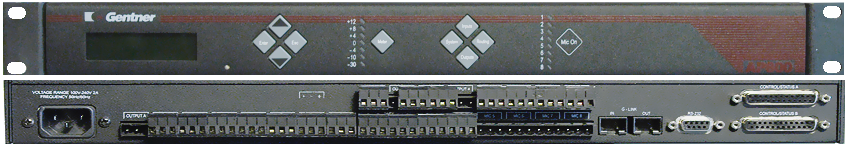
\includegraphics[width=1\textwidth]{images/gentner-ap-800.png}
\caption{Gentner AP-800 echo cancellation device.}
\label{fig:Gentner}
\end{figure}

%%%%%%%%%%%%%%%%%%%%%%%%%%%%%%%%%%%%%%%%%%%%%%%%%%%%%%%%%%%%%%%%%%%%%
%%%%%%%%%%%%%%%%%%%%%%%%%%%%%%%%%%%%%%%%%%%%%%%%%%%%%%%%%%%%%%%%%%%%%
\section{Videoconferencing room}
%%%%%%%%%%%%%%%%%%%%%%%%%%%%%%%%%%%%%%%%%%%%%%%%%%%%%%%%%%%%%%%%%%%%%
%%%%%%%%%%%%%%%%%%%%%%%%%%%%%%%%%%%%%%%%%%%%%%%%%%%%%%%%%%%%%%%%%%%%%

The room we chose for AccessGrid had originally served as an office for the organisation. We therefore had to work within certain constraints, since its original function had to be preserved. Our approach demonstrates that other organisations can follow a similar path at minimal cost. The main changes were:
\begin{paklist}
%-----------------------
\item Preparing projection surfaces by using two walls, which had to be repainted with a fresh coat of white paint.
%-----------------------
\item Installing loudspeakers in the corners of the room.
%-----------------------
\item Installing additional spotlights in one corner of the room.
%-----------------------
\item Installing a cabling system consisting of VGA (computer--projector), S-Video (camera--computer), STP (computer--switch) and audio (microphone--mixer, amplifier--speakers) connections.
\end{paklist}

\begin{figure}
\centering
\includesvg[width=1\textwidth]{arch-ciant-ag-room}
\caption{Room used for videoconferencing.}
\label{fig:CIANT-AG-room}
\end{figure}

Figure \ref{fig:CIANT-AG-room}(A) shows the layout of objects in the room. For video projection, we used two white walls (6a, 6b). Projection is provided by three projectors (5a, 5b), as shown in Figure \ref{fig:CIANT-AG-room}(C), connected to the AG-Display computer (8). The microphone (2) is positioned at the front of the room. It captures sound over a sufficiently wide angle, as also shown in Figure \ref{fig:CIANT-AG-room}(D), together with the arrangement of the loudspeakers (7a, 7b, 7c) in the corners of the room. Microphone audio is sent through the audio mixer (3) directly to the AG-AudioVideo computer (8). Correct operation of the echo-cancellation device (Gentner AP-800) is essential. Figure \ref{fig:CIANT-AG-room}(D) makes it clear that the microphone captures a substantial amount of sound from the loudspeakers, which would otherwise cause unpleasant echo at all connected nodes.

Because of its limited size, the room can accommodate no more than 15 people. This has not yet proved to be a problem, since we have not reached that number. Participants are divided into two categories: active and passive. Active participants sit at the front of the room, around the microphone (2). The moderator sits at position (1). This also determines the arrangement of the cameras (4a, 4b), shown in Figure \ref{fig:CIANT-AG-room}(B). The main camera (4a) captures the moderator and the people closest to them. The secondary camera (4b) captures most of the audience. The operator sits at position (8) and is responsible for the technical operation of the conference. In case of problems, the operator communicates with the other operators using text messages.

%%%%%%%%%%%%%%%%%%%%%%%%%%%%%%%%%%%%%%%%%%%%%%%%%%%%%%%%%%%%%%%%%%%%%
%%%%%%%%%%%%%%%%%%%%%%%%%%%%%%%%%%%%%%%%%%%%%%%%%%%%%%%%%%%%%%%%%%%%%
\section{Day-to-day operational experience}\label{kap:CiantSkusenosti}
%%%%%%%%%%%%%%%%%%%%%%%%%%%%%%%%%%%%%%%%%%%%%%%%%%%%%%%%%%%%%%%%%%%%%
%%%%%%%%%%%%%%%%%%%%%%%%%%%%%%%%%%%%%%%%%%%%%%%%%%%%%%%%%%%%%%%%%%%%%

Originally, we planned to use three projectors. The two main projectors were intended to display video from the VIC application, while the third would display the AG-Display computer's controls and shared presentations.
After several conferences, however, we found that two projectors were sufficient. Moreover, the recording method we used at the time could capture the image from only one projector.

Despite their simplicity and limitations, our first attempts at recording conferences proved very useful. The results can be viewed on the project's wiki pages \cite{CIANT-AGnodeWiki}, including recordings of the Polylogues conferences mentioned above \cite{CIANT-Polylogues-1}, \cite{CIANT-Polylogues-2} and \cite{CIANT-Polylogues-3}.

Recording worked by using the graphics card's ability to clone the image from one VGA output to an S-Video output. We connected this signal to a digital video camera and recorded it onto Mini-DV tapes. After the conference, we digitised the recording into an FLV or MPEG file.

The main advantages of this solution are its simplicity and the fact that it does not interfere with the conference at the software level. We do not need to process the RTP packet stream, and problems caused by increased latency and jitter are avoided. The result is a Mini-DV tape, which also serves as a suitable backup medium.

There are several disadvantages, however. The image from the graphics card, delivered as an S-Video signal, has a maximum resolution of 1024x768. This resolution is already hardware-scaled to 800x600, so the recorded image is slightly lower in quality than the original image displayed on the projection screen.
The resulting recording does not take full advantage of AccessGrid technology. Furthermore, this method can record the image from only one projector. We addressed this limitation by simply not using the additional projectors, or by displaying less important content on them. In that case, the conference operator must decide which video signals and shared presentations are most important. This increases the operator's cognitive load: in addition to managing the technical operation, they must also pay attention to the content of the conference. This can be particularly demanding when the conference deals with a subject that is unfamiliar to the operator.

Another disadvantage is the need to convert the Mini-DV format to MPEG afterwards. This solution also does not allow stored data streams to be played directly in a new conference. All elements are mixed into a single audio-video recording, just as participants saw them through the projection system.

As mentioned above, our room can accommodate 15 people. In such a crowded space, adequate ventilation is necessary, but our solution essentially ignores this requirement. Ventilation is handled in a simple way by opening a window. During our first transmissions, however, we encountered a problem: noise and light from outside disturbed the sensitive conditions inside the room. Opening the window was therefore not an option, and participants had to endure uncomfortable heat and stale air.

Room lighting is another important factor. On the one hand, a dark environment is desirable for projection. On the other hand, the cameras need sufficient light to capture the participants. We resolved this conflict in favour of better lighting. A dark environment not only reduces image quality and makes participants sleepy, but also increases the video bitrate. In poor lighting conditions, the camera introduces random image artefacts that make the image more difficult to encode.

When installing the cabling, we had to ensure that the individual components were properly shielded. We found that running VGA cables alongside power and S-Video cables could cause interference and distort the image.
\proofed

		%%%%%%%%%%%%%%%%%%%%%%%%%%%%%%%%%%%%%%%%%%%%%%%%%%%%%%%%%%%%%%%%%%%%%
%%%%%%%%%%%%%%%%%%%%%%%%%%%%%%%%%%%%%%%%%%%%%%%%%%%%%%%%%%%%%%%%%%%%%
%%%%%%%%%%%%%%%%%%%%%%%%%%%%%%%%%%%%%%%%%%%%%%%%%%%%%%%%%%%%%%%%%%%%%
%%%%%%%%%%%%%%%%%%%%%%%%%%%%%%%%%%%%%%%%%%%%%%%%%%%%%%%%%%%%%%%%%%%%%
\chapter{NAT/Firewall}\index{NAT!problem}
%%%%%%%%%%%%%%%%%%%%%%%%%%%%%%%%%%%%%%%%%%%%%%%%%%%%%%%%%%%%%%%%%%%%%
%%%%%%%%%%%%%%%%%%%%%%%%%%%%%%%%%%%%%%%%%%%%%%%%%%%%%%%%%%%%%%%%%%%%%
%%%%%%%%%%%%%%%%%%%%%%%%%%%%%%%%%%%%%%%%%%%%%%%%%%%%%%%%%%%%%%%%%%%%%
%%%%%%%%%%%%%%%%%%%%%%%%%%%%%%%%%%%%%%%%%%%%%%%%%%%%%%%%%%%%%%%%%%%%%

We use RFC 3022 \cite{RFC-3022-NAT} (Traditional IP Network Address Translator) as the main reference in this chapter.

Network Address Translation (NAT) is a technique for overcoming the 32-bit limit of the IPv4 address space in the TCP/IP protocol design.
It allows IP addresses to be reused within a private local network.
Communication with the outside world is achieved through a gateway with two network interfaces: one with a private IP address and the other with a public IP address.

The gateway manages the translation process, also known as NAT, which is depicted in Figure \ref{fig:NatArchitecture}.
The main element of this mechanism is \textbf{a mapping table}, which stores information about the mapping of packet flows between private addresses and ports on the two interfaces.
The NAT mechanism modifies the packet contents in the following fields:
\begin{paklist}
\item source address and port (when a packet moves from the private to the public network),
\item destination address and port (in the reverse direction, from the public to the private network),
\item checksum (recalculated over the modified packet).
\end{paklist}

When a packet leaves the private network, its \textbf{source address} is replaced with the gateway's \textbf{public address}.
The receiver can see only the public address and therefore sends its response to the gateway's IP address.
On the return path, the packet's destination IP address is translated again according to the mapping table and the packet is delivered to the original node inside the private network.
The NAT mechanism must recalculate the packet checksum because the packet has been modified.

\begin{figure}
\centering
\includesvg[width=1\textwidth]{nat-architecture}
\caption{NAT architecture.}
\label{fig:NatArchitecture}
\end{figure}

%%%%%%%%%%%%%%%%%%%%%%%%%%%%%%%%%%%%%%%%%%%%%%%%%%%%%%%%%%%%%%%%%%%%%
%%%%%%%%%%%%%%%%%%%%%%%%%%%%%%%%%%%%%%%%%%%%%%%%%%%%%%%%%%%%%%%%%%%%%
\section{NAT-related issues}
%%%%%%%%%%%%%%%%%%%%%%%%%%%%%%%%%%%%%%%%%%%%%%%%%%%%%%%%%%%%%%%%%%%%%
%%%%%%%%%%%%%%%%%%%%%%%%%%%%%%%%%%%%%%%%%%%%%%%%%%%%%%%%%%%%%%%%%%%%%
Address translation modifies only the IP packet header and does not touch the payload.
It is clear that such a mechanism cannot handle protocols that include routing information in the payload, a limitation that is even more significant when packets are encrypted.

NAT allows communication to be initiated by nodes inside the private network. Communication initiated in the opposite direction is not directly possible.
Although this is a drawback, the principle can also be considered a security feature.
In our case, however, we would like to connect nodes transparently. We will describe the QuickBridge tool later in this thesis.
Packets arriving at the gateway from the public network are forwarded only if a corresponding entry exists in the NAT mapping table.
One possible workaround is to initialise the mapping entry by periodically sending dummy packets to the outside network (keep-alive).
This solution, however, does not work with all types of NAT.

%%%%%%%%%%%%%%%%%%%%%%%%%%%%%%%%%%%%%%%%%%%%%%%%%%%%%%%%%%%%%%%%%%%%%
%%%%%%%%%%%%%%%%%%%%%%%%%%%%%%%%%%%%%%%%%%%%%%%%%%%%%%%%%%%%%%%%%%%%%
\section{A simple NAT-traversal test}
%%%%%%%%%%%%%%%%%%%%%%%%%%%%%%%%%%%%%%%%%%%%%%%%%%%%%%%%%%%%%%%%%%%%%
%%%%%%%%%%%%%%%%%%%%%%%%%%%%%%%%%%%%%%%%%%%%%%%%%%%%%%%%%%%%%%%%%%%%%
The NAT traversal mechanism can be tested as follows.
Our test configuration consists of three components: a gateway, a server and a client.

\paragraph*{NAT gateway:}
A Linux machine with two network cards: \verb|$NAT_PUB_DEV|, with IP address \verb|$NAT_PUB_IP|, connected to the public network, and \verb|$NAT_PRIV_DEV|, with IP address \verb|$NAT_PRIV_IP|, connected to the private network. NAT is enabled on the \verb|$NAT_PUB_DEV| interface using the \textbf{iptables} tool.

\paragraph*{Server with a public IP address:}
The public IP address is \verb|$SERVER_IP|. For testing, we use \textbf{netcat}, which can create a UDP server listening on port \verb|$SERVER_PORT|. The contents of each packet are written to standard output (stdout), while data read from standard input (stdin) is sent as a UDP packet to the same address and port.

\paragraph*{Client with a private IP address:}
The client is located in the private network and has IP address \verb|$CLIENT_IP|. Its network interface parameters are assigned automatically using DHCP, and its \textbf{default gateway} is set to \verb|NAT_PRIV_IP|. We again use \textbf{netcat} to facilitate UDP communication through stdin and stdout.

\bigskip
The first UDP packet sent from the node with a private IP address to the server with a public IP address creates a path for subsequent UDP communication in both directions. As described above, NAT translates packets according to the mapping entry that has been created.
This path usually disappears when the NAT gateway is restarted or when the mapping entry expires due to a timeout.

\begin{verbatim}
# gateway: enable NAT
iptables -t nat -A POSTROUTING -j MASQUERADE -o $NAT_PUB_DEV

# server: test connectivity
ping $NAT_PUB_IP

# server: listen for UDP packets
netcat -lup $SERVER_PORT

# client: connect to the server
netcat -u $SERVER_IP $SERVER_PORT
\end{verbatim}

%%%%%%%%%%%%%%%%%%%%%%%%%%%%%%%%%%%%%%%%%%%%%%%%%%%%%%%%%%%%%%%%%%%%%
%%%%%%%%%%%%%%%%%%%%%%%%%%%%%%%%%%%%%%%%%%%%%%%%%%%%%%%%%%%%%%%%%%%%%
\section{Tunneling}
%%%%%%%%%%%%%%%%%%%%%%%%%%%%%%%%%%%%%%%%%%%%%%%%%%%%%%%%%%%%%%%%%%%%%
%%%%%%%%%%%%%%%%%%%%%%%%%%%%%%%%%%%%%%%%%%%%%%%%%%%%%%%%%%%%%%%%%%%%%

In the previous test, we demonstrated a simple NAT traversal solution in which communication is initiated from within the private network and then continues bidirectionally over a single TCP or UDP port.
If we could encapsulate our communication in a single packet stream, we would be able to \textbf{tunnel} arbitrary communication between two nodes.
Such a hypothetical tunnel could provide the following services:
\begin{paklist}
\item encrypted communication,
\item reliable delivery,
\item transparent tunneling,
\item tunneling of multicast packets,
\item tunneling of other protocols, such as IPX,
\item and more \ldots
\end{paklist}

For multimedia streaming, an unreliable delivery service is usually the best solution. Additional layers, such as encryption, could have a negative impact on system latency.
Through AGConnector, AccessGrid supports multicast tunneling using the UMTP protocol.

\subsection{NAT-to-NAT communication}

So far, we have considered situations in which a client in a NAT-protected network communicates with a public server.
However, it is also possible to address the case of two NAT-protected nodes located in separate networks.

In the following example, the \textbf{nat-traverse} tool is used together with the PPP protocol to create a tunnel. NAT on both sides must preserve port numbers.
The example shows a NAT gateway \verb|\${CLIENT_IP}| for the client and a NAT gateway \verb|\${CLIENT_IP}| for the server.
Both parties exchange UDP packets through port 40000.

\begin{verbatim}
# client: create the ppp0 interface
nat-traverse --cmd="pppd updetach noauth passive notty ipparam \
  vpn 10.0.0.1:10.0.0.2" 40000:\${CLIENT_IP}:40000
\end{verbatim}

\begin{verbatim}
# server: accept the PPP connection
nat-traverse --cmd="pppd nodetach notty noauth" \
  40000:\${SERVER_IP}:40000
\end{verbatim}

After the tunnel has been established, routing tables must be configured on both sides.
QuickBridge packets can be sent through the tunnel. Alternatively, multicast packets can be tunnelled, but this requires the installation of a multicast router.
The configuration also requires administrative privileges so that the PPP network interface (typically \verb|ppp0|) can be created.

\begin{verbatim}
# client: route multicast packets through the tunnel
route add -net 224.0.0.0 netmask 255.0.0.0 gw ppp0
route add -net 239.0.0.0 netmask 255.0.0.0 gw ppp0
\end{verbatim}

\begin{verbatim}
# server: enable packet forwarding and start the multicast router
echo 1 > /proc/sys/net/ipv4/ip_forward
mrouted
\end{verbatim}

The nat-traverse application can be used with OpenVPN as well as PPP, allowing the entire communication to be encrypted.
\proofed

		%%%%%%%%%%%%%%%%%%%%%%%%%%%%%%%%%%%%%%%%%%%%%%%%%%%%%%%%%%%%%%%%%%%%%
%%%%%%%%%%%%%%%%%%%%%%%%%%%%%%%%%%%%%%%%%%%%%%%%%%%%%%%%%%%%%%%%%%%%%
%%%%%%%%%%%%%%%%%%%%%%%%%%%%%%%%%%%%%%%%%%%%%%%%%%%%%%%%%%%%%%%%%%%%%
%%%%%%%%%%%%%%%%%%%%%%%%%%%%%%%%%%%%%%%%%%%%%%%%%%%%%%%%%%%%%%%%%%%%%
\chapter{Linux-only AccessGrid}\label{kap:LinuxNode}
%%%%%%%%%%%%%%%%%%%%%%%%%%%%%%%%%%%%%%%%%%%%%%%%%%%%%%%%%%%%%%%%%%%%%
%%%%%%%%%%%%%%%%%%%%%%%%%%%%%%%%%%%%%%%%%%%%%%%%%%%%%%%%%%%%%%%%%%%%%
%%%%%%%%%%%%%%%%%%%%%%%%%%%%%%%%%%%%%%%%%%%%%%%%%%%%%%%%%%%%%%%%%%%%%
%%%%%%%%%%%%%%%%%%%%%%%%%%%%%%%%%%%%%%%%%%%%%%%%%%%%%%%%%%%%%%%%%%%%%

V~tejto kapitole popíšeme výstavbu uzla založeného na voľne dostupných komponentoch. Ako základ architektúry použijeme existujúci AG uzol v~organizácii Ciant. Naším príspevkom pre AG komunitu je niekoľko aplikácií voľne dostupných na wiki-stránkach projektu \cite{CIANT-AGnodeWiki}. V súvislosti so zdieľanými aplikáciami spomenieme hlavne SharedMPlayer.

\paragraph*{Fundamental rules:}
\begin{paklist}
\item Znížiť množstvo potrebného hardwaru na minimum.
\item Sprístupniť pripojenie uzlom za firewallom a NAT.
\item Využiť operačný systém Linux a voľne dostupné komponenty.
\end{paklist}

%%%%%%%%%%%%%%%%%%%%%%%%%%%%%%%%%%%%%%%%%%%%%%%%%%%%%%%%%%%%%%%%%%%%%
%%%%%%%%%%%%%%%%%%%%%%%%%%%%%%%%%%%%%%%%%%%%%%%%%%%%%%%%%%%%%%%%%%%%%
\section{Emplacement}
%%%%%%%%%%%%%%%%%%%%%%%%%%%%%%%%%%%%%%%%%%%%%%%%%%%%%%%%%%%%%%%%%%%%%
%%%%%%%%%%%%%%%%%%%%%%%%%%%%%%%%%%%%%%%%%%%%%%%%%%%%%%%%%%%%%%%%%%%%%

Podľa E. Hladkej a P. Holuba \cite{ArticleUVTMU-KomunikaceAGPoint}, je potrebné pred implementáciou videokonferenčného uzla zvážiť jeho priestorovú náročnosť. Uvádza sa \cite{AG-MinimumReqirements}, že je potrebné vyhradiť miesto aspoň pre troch účastníkov, počítače a projekčnú techniku. Inak nemá zmysel uvažovať o~jeho vytvorení. Musíme však rozlišovať medzi plnohodnotným videokonferenčným uzlom, mobilným videokonferenčným uzlom \cite{ArticleUVTMU-MobilniUzelAG} a tzv. personal interface to grid (PIG), ktorý má zabezpečiť pripojenie pre jednotlivcov bez použitia drahej projekčnej techniky. Rozdiely sú hlavne v~množstve potrebného hardware. Zatiaľ čo pri výstavbe plnohodnotného alebo mobilného uzla uvažujeme o~použití niekoľkých projektorov, v~prípade AG PIG vystačí účastník aj s~jedným prenosným počítačom dokonca bez vlastnej kamery a mikrofónu. Má teda na výber, či chce pasívne sledovať vysielanie, alebo prispievať aj vlastnými dátovými tokmi. Ďalej sa uvádza, aké problémy môžu vzniknúť pri komunikácii účastníkov z~rôznych časových pásiem. Aby sme zmiernili účinky únavy, musia sa účastníci cítiť v~miestnosti pohodlne, čo môžeme ovplyvniť správnym výberom nábytku a osvetlenia.

%%%%%%%%%%%%%%%%%%%%%%%%%%%%%%%%%%%%%%%%%%%%%%%%%%%%%%%%%%%%%%%%%%%%%
%%%%%%%%%%%%%%%%%%%%%%%%%%%%%%%%%%%%%%%%%%%%%%%%%%%%%%%%%%%%%%%%%%%%%
\section{Network connectivity}
%%%%%%%%%%%%%%%%%%%%%%%%%%%%%%%%%%%%%%%%%%%%%%%%%%%%%%%%%%%%%%%%%%%%%
%%%%%%%%%%%%%%%%%%%%%%%%%%%%%%%%%%%%%%%%%%%%%%%%%%%%%%%%%%%%%%%%%%%%%

Pre rozhranie PIG (Personal Interface to Grid) stačí použiť sieť s~kapacitou okolo 1Mbit/s. Pre plnohodný uzol je táto hodnota niekoľkonásobne vyššia, odporúča sa aspoň 10Mbit/s.
V~prípade PIG rozhrania môže účastník využiť unicastové pripojenie cez premostenie (ak existuje), v~prípade plnohodnotného uzla sa vyžaduje kvalitné multicastové pripojenie.

%%%%%%%%%%%%%%%%%%%%%%%%%%%%%%%%%%%%%%%%%%%%%%%%%%%%%%%%%%%%%%%%%%%%%
%%%%%%%%%%%%%%%%%%%%%%%%%%%%%%%%%%%%%%%%%%%%%%%%%%%%%%%%%%%%%%%%%%%%%
\section{Hardware}
%%%%%%%%%%%%%%%%%%%%%%%%%%%%%%%%%%%%%%%%%%%%%%%%%%%%%%%%%%%%%%%%%%%%%
%%%%%%%%%%%%%%%%%%%%%%%%%%%%%%%%%%%%%%%%%%%%%%%%%%%%%%%%%%%%%%%%%%%%%

Venujme sa teraz hardwaru, ktorý je potrebný na výstavbu plnohodnotného uzla. Hardwarová konfigurácia môže vychádzať z~architektúry, ktorú sme popísali v~kapitole \ref{kap:CiantAGKomponenty}. Použijeme teda počítač AG-Display na zobrazovanie pomocou projektorov, AG-AudioVideo na kódovanie obrazu a kódovanie/dekódovanie zvuku a počítač AG-Bridge na premostenie multicastu. Z~použitých komponentov je dôležité zakúpiť niekoľko kariet na digitalizáciu obrazu pre počítač AG-AudioVideo a niekoľko grafických kariet pre AG-Display. V~prípade, že chceme používať multicastovú sieť, nevyhneme sa nákupu sieťového prepínača\footnote{Je možné použiť namiesto tohto špecializovaného hardware počítač s~niekoľkými sieťovými kartami a s~podporou multicast routingu v~jadre operačného systému. Z~dôvodu latencie, spoľahlivosti a spotreby elektrickej energie však odporúčame použiť hardwarový prepínač.} (switch) s~podporou protokolu IGMP (kapitola \ref{kap:Multicast}).

V~prípade, že použijeme sluchátka s~mikrofónom pre každého účastníka konferencie, nemusíme investovať finančné prostriedky do nákupu zariadenia na odstraňovanie spätnej väzby. Musíme si však uvedomiť, že sa tým zníži celkové pohodlie účastníkov. V~oboch prípadoch je dôležité dôkladne skontrolovať kvalitu zvuku. Nestačí, že počujeme ostatných účastníkov konferencie. Musíme zabezpečiť, aby aj zvuk z~nášho uzla bol v~dobrej kvalite.

Čo sa týka projekčnej techniky, odporúčame použiť aspoň dva projektory. Jeden bude slúžiť pre projekciu snímkov z~prezentácie, druhý bude zobrazovať obrazy účastníkov.

Pred nákupom odporúčame preštudovať stránky accessgrid.org, hlavne databázu hardware \cite{AG-HardwareDatabase}, ktorú vytvorili členovia AG komunity. Stránky poskytujú prehľad o~konkrétnych hardwarových prvkoch, akými sú videokamery, webkamery, mikrofóny, zvukové karty, projektory a mnoho ďalších, vrátane ich parametrov, fotografií a odkazov na stránky výrobcu.

\paragraph*{Important notice:}
Multicastový most musí byť inštalovaný na osobitnom počítači. V~prípade, že z~jedného socketu čítajú dáta dva procesy, získa tieto dáta posledný proces, ktorý otvoril socket systémovým volaním \verb|bind()|. Riešením by bolo zrkadlenie paketov istou formou proxy servera implementovaného ako user-space proces alebo priamo v~jadre operačného systému.


%%%%%%%%%%%%%%%%%%%%%%%%%%%%%%%%%%%%%%%%%%%%%%%%%%%%%%%%%%%%%%%%%%%%%
%%%%%%%%%%%%%%%%%%%%%%%%%%%%%%%%%%%%%%%%%%%%%%%%%%%%%%%%%%%%%%%%%%%%%
\section{Operating system and esential software}
%%%%%%%%%%%%%%%%%%%%%%%%%%%%%%%%%%%%%%%%%%%%%%%%%%%%%%%%%%%%%%%%%%%%%
%%%%%%%%%%%%%%%%%%%%%%%%%%%%%%%%%%%%%%%%%%%%%%%%%%%%%%%%%%%%%%%%%%%%%

AccessGrid ako multiplatformná aplikácia existuje v~rôznych obmenách pre niekoľko najvýznamnejších operačných systémov vrátane Windows, Linux, FreeBSD, MacOS. Pre nás zaujímavým, je operačný systém Linux. Pri výbere distribúcie hrala hlavnú úlohu dostupnosť inštalačných balíkov. Aj keď oficiálnu podporu má distribúcia Fedora, dali sme prednosť OpenSuse 10.0 na základe skúseností s~uzlom v~organizácii Ciant, kde používame OpenSuse 9.3.

\paragraph*{Installed packages:}
\begin{paklist}
\item AccessGrid-2.4-5
\item MPlayer-1.0rc1try2-2.pm.1
\item xorg-x11-Xvnc-6.8.2-100
\item agvcr-2.1.4-1
\item + všetky potrebné závislosti
\end{paklist}

Druhým použitým systémom je Debian GNU/Linux 3.1. Z~pohľadu AG 2.4 nie je táto voľba najšťastnejšia, pretože inštalačné balíky existujú iba pre príbuznú distribúciu Ubuntu. Bolo však potrebné využiť existujúci server, na ktorom, okrem iného beží aj wiki-stránka projektu Ciant AG node. Server je v~súčasnej dobe umiestnený na adrese \url{ciant114.cesnet.cz}.

\paragraph*{Installed packages:}
\begin{paklist}
\item accessgrid2.4-1.4 (z~distribúcie Ubuntu)
\item + všetky potrebné závislosti
\end{paklist}

%%%%%%%%%%%%%%%%%%%%%%%%%%%%%%%%%%%%%%%%%%%%%%%%%%%%%%%%%%%%%%%%%%%%%
%%%%%%%%%%%%%%%%%%%%%%%%%%%%%%%%%%%%%%%%%%%%%%%%%%%%%%%%%%%%%%%%%%%%%
\section{Video and audio transmission}
%%%%%%%%%%%%%%%%%%%%%%%%%%%%%%%%%%%%%%%%%%%%%%%%%%%%%%%%%%%%%%%%%%%%%
%%%%%%%%%%%%%%%%%%%%%%%%%%%%%%%%%%%%%%%%%%%%%%%%%%%%%%%%%%%%%%%%%%%%%

Jednou z~najdôležitejších súčastí AG sú tzv. MBone tools, nástroje pre komunikáciu pomocou multicastovej siete. V~rôznych obmenách sa používajú aj v~systémoch VRVS a InSORS. Ide o~aplikácie určené na prenos obrazu, zvuku a zdieľanie textových dokumentov, kde dátové prenosy sú uskutočňované pomocou multicastového rozšírenia IPv4 protokolu (kapitola \ref{kap:Multicast}). Rozdiely medzi rôznymi verziami sú hlavne v~množstve podporovaných kodekov a vo vzhľade užívateľského rozhrania.

Ak chceme využiť tieto nástroje mimo AccessGrid, sú k~dispozícii na adrese ktorú uvádzame v~použitej literatúre pod označením \cite{Original-MBone-Tools-Download}, pre praktické použitie však odporúčame využiť niektorú s~ponúkaných modifikácií. Niekoľko odskúšaných verzií sme záujemcom pripravili na stránkach projektu Ciant AG node \cite{CIANT-AGnodeWiki}, ako súčasť tejto diplomovej práce.

\subsection{OpenMash framework}\label{kap:OpenMash}
Open Mash \cite{OpenMashProject} bol navrhnutý pre vedeckú komunitu ako dôsledok potreby práce s~multimediálnymi dátovými tokmi v~rámci videokonferenčných systémov. Tento balík bol navrhnutý s~ohľadom na preklenutie problémov, ktoré sa objavovali v~podobných, starších systémoch. Išlo hlavne o~ich slabú prenositeľnosť do iných operačných systémov, než pre ktoré boli navrhnuté, nedostupnosť zdrojového kódu a neúplná alebo len malá podpora IETF protokolov. Idea vzniku tejto aplikácie pochádza od Larry Rowa a Steve McCanna. Vznik sa datuje do roku 1999. Aplikačný balík OpenMash (re)implementuje projekty ako sdr, nv, vic, vat, wb, mtrace vyvíjaných v~komunite MBone.

Po implementačnej stránke je OpenMash riešený ako kombinácia jazyka C/C++ s jazykom TCL/Tk \cite{WIKI-TCL-TK}. TCL je jednoduchý ale veľmi silný skritpovací jazyk určený nielen pre prototypovanie aplikácií ale aj pre vývoj skutočne prenostiteľných systémov. Jeho multiplatformná grafická nadstavba Tk sa používa aj v~iných jazykoch, napríklad Python. OpenMash navyše používa ďalšie rozšírenie -- OTCL \cite{OTcl-Extension}, ktoré pridáva podporu objektov do inak funkcionálneho jazyka. Zatiaľ čo jazyk C++ je použitý pre výpočtovo náročné procedúry, interpretovaný jazyk TCL/Tk je vhodný ako spojovací nástroj a pre interakciu s~užívateľom pomocou grafického rozhrania.

OpenMash je dostupný pre všetky hlavné platformy, čo z~neho robí ideálny nástroj pre multiplatformné videokonferenčné riešenie. Tejto skutočnosti si boli vedomí aj tvorcovia úspešného videokonferenčného systému VRVS\index{VRVS!OpenMash} a EVO, ktorý sme popísali v~kapitole \ref{kap:VRVS}. Autori použili OpenMash pre aplikácie na prenos obrazu a zvuku.

Jazyk TCL/Tk nám umožnil modifikovať existujúce aplikácie VIC-VRVS a VIEVO z~projektu VRVS A~EVO a vytvoriť novú aplikáciu EVIC, ktorú poskytujeme záujemcom na stránkach Ciant AG node \cite{CIANT-AGnodeWiki}.

\subsection{VIC}\label{kap:VIC}
Video Conferencing Tool (VIC) umožňuje prenos obrazu v~reálnom čase pomocou protokolu RTP, ktorý uvádzame v~kapitole \ref{kap:RTP+RTCP}. Prenos zvuku však musí byť riešený inou aplikáciou. Obsahuje podporu pre niekoľko kodekov a ich množstvo a kvalita implementácie sa líši v~závislosti na verzii. Asi najstabilnejšími verziami sú VIC-2.8ucl1.1.3 z~balíka AG a VIC z~projektu OpenMash. VIC umožňuje viacbodovú komunikáciu s~využitím multicastovej siete. Špeciálnym prípadom, ktorý využijeme, je možnosť posielať RTP pakety na sieťové loopback zariadenie (localhost). To nám umožní prípravu prezentácie, jej nahrávanie a opätovné zdieľanie v~konferencii. Obsah RTP paketov je možné pred odoslaním zakódovať a zvýšiť tak bezpečnosť prenosu. Potenciálny útočník ale stále vidí odosielateľa a príjemcu RTP paketu, ako aj množstvo ďalších "užitočných" informácií. Implicitným kodekom je H.261. Ako uvádzame v~kapitole \ref{kap:H.261}, tento kodek je až 3-krát efektívnejší ako pôvodný kodek NV. Ďalšími významnými kodekmi sú H.263 a H.263+ (kapitola \ref{kap:H.263}), ktoré ale v~niektorých verziách VICu spôsobujú pád aplikácie. To sa našťastie netýka verzie založenej na OpenMash, ktorý chceme využívať. Existuje aj vývojová verzia VICu s~podporou kodeku H.264 (kapitola \ref{kap:H.264}).

\begin{figure}
\centering
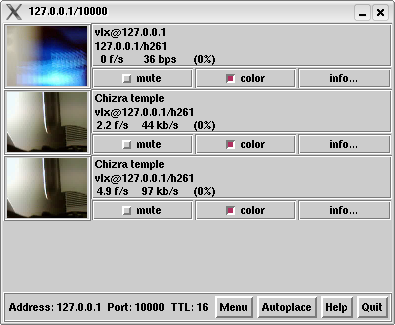
\includegraphics[width=0.3\textwidth]{images/video-app-vic-ucl}
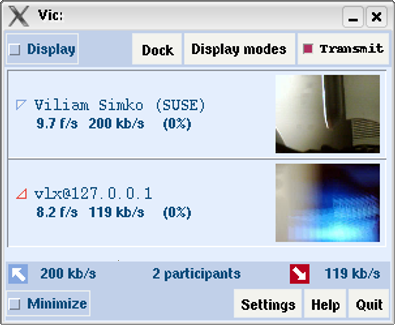
\includegraphics[width=0.3\textwidth]{images/video-app-vic-vrvs}
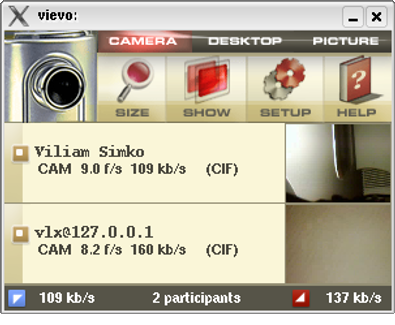
\includegraphics[width=0.3\textwidth]{images/video-app-vievo}
\caption{Aplikácie určené na prenos obrazu (vic-ucl, vic-vrvs, vievo).}
\label{fig:MBoneVideoApplications}
\end{figure}

Na obrázku \ref{fig:MBoneVideoApplications} vidíme rôzne verzie aplikácie VIC. Vľavo je originálna verzia VIC-2.8ucl1.1.3, v~strede verzia zo systému VRVS založená na upravenom OpenMash 6.1 a vpravo je značne upravená verzia z~projektu EVO, ktorá však nepatrí medzi open-source software. Tento problém sa čiastočne pokúšame riešiť reimplementáciou v~aplikácii EVIC.


\subsection{RAT}\label{kap:RAT}
Robust Audio Tool (RAT) je podobne ako aplikácia VIC určená na prenos multimediálneho obsahu v~reálnom čase pomocou RTP paketov medzi úžastníkmi multicastovej skupiny. Multimediálnym obsahom je v~prípade RATu zvuk. K~dispozícii je niekoľko zvukových kodekov, ako napr. GSM, L16 a dokonca v~niektorých verziách aj MP3. Líšia sa medzi sebou kvalitou zvuku a spotrebou prenosového pásma. Podobne ako VIC, aj RAT podporuje šifrovanie RTP obsahu a vyskytuje sa v~niekoľkých verziách, ktorých príklady vidíme na obrázku \ref{fig:MBoneAudioApplications}. Vpravo pôvodná aplikácia VAT, ktorá umožňovala prenos zvuku a obrazu súčasne, v~strede originálna verzia RAT z~balíka AG a vpravo verzia z~projektu VRVS.

V~kapitole \ref{kap:HybridRAT} je popísaná hybridná verzia aplikácie RAT, ktorá vznikla spojením zdrojových kódov z~projektu RAT-VRVS a RAT-UCL a umožňuje nahrávať zvuk pomocou sieťového loopback zariadenia (localhost). Takto opravenú verziu ponúkame záujemcom na stránkach Ciant AG node \cite{CIANT-AGnodeWiki}.

\begin{figure}
\centering
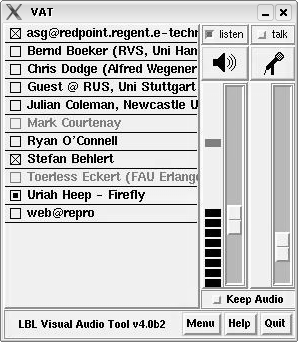
\includegraphics[width=0.3\textwidth]{images/audio-app-vat.png}
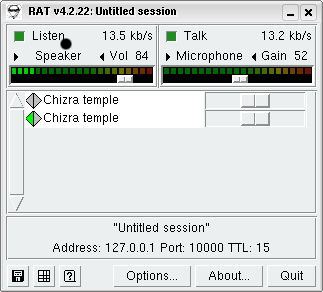
\includegraphics[width=0.3\textwidth]{images/audio-app-rat.png}
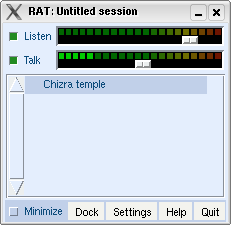
\includegraphics[width=0.3\textwidth]{images/audio-app-rat-vrvs.png}
\caption{Aplikácie určené na prenos zvuku (vat, rat, rat-vrvs).}
\label{fig:MBoneAudioApplications}
\end{figure}


%%%%%%%%%%%%%%%%%%%%%%%%%%%%%%%%%%%%%%%%%%%%%%%%%%%%%%%%%%%%%%%%%%%%%
%%%%%%%%%%%%%%%%%%%%%%%%%%%%%%%%%%%%%%%%%%%%%%%%%%%%%%%%%%%%%%%%%%%%%
\section{Shared applications}
%%%%%%%%%%%%%%%%%%%%%%%%%%%%%%%%%%%%%%%%%%%%%%%%%%%%%%%%%%%%%%%%%%%%%
%%%%%%%%%%%%%%%%%%%%%%%%%%%%%%%%%%%%%%%%%%%%%%%%%%%%%%%%%%%%%%%%%%%%%

Už v~základnej inštalácii AG sa nachádza niekoľko zdieľaných aplikácií a navyše je možné túto množinu rozšíriť pomocou jazyka Python. Architektúra zideľaných aplikácií je zázornená na obrázku \ref{fig:ArchAGSharedApp}. AG Toolkit poskytuje triedu SharedAppClient, ktorá implementuje všetky operácie potrebné pre komunikáciu pomocou zbernice Event Channel. Trieda uľahčuje doručovanie správ a synchronizáciu klientov. Komunikácia medzi klientami (Application Client) prebieha pomocou XML-RPC.

\begin{figure}
\centering
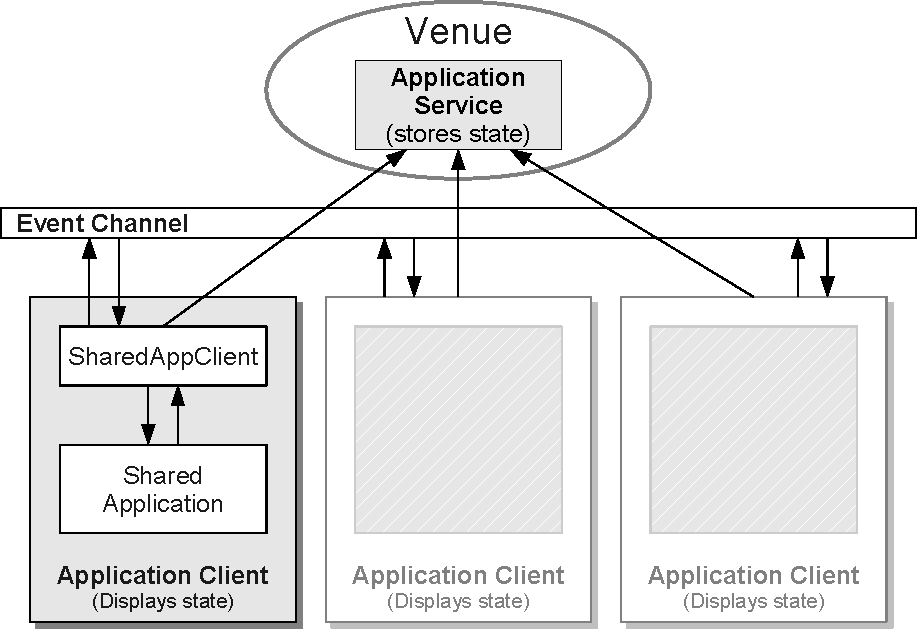
\includegraphics[width=0.8\textwidth]{images/arch-ag-sharedapp}
\caption{Architektúra zdieľaných aplikácií AccessGridu.}
\label{fig:ArchAGSharedApp}
\end{figure}

Ďalším prostriedkom pre vytvorenie zdieľaného prostredia je Virtual Network Computing (VNC) \cite{MAN-Virtual-Network-Computing}. Systém využíva Remote Frame Buffer protokol (RFB) \cite{MAN-RFB-Protocol}. Protokol prenáša informácie o~zmenách na zdieľanej obrazovke a informáciách o~stlačených klávesách a tlačítkach myši. Jeho serverová aj klientská časť je platformovo nezávislá. Protokol RFB je bezstavový a na server môže byť súčasne pripojených niekoľko užívateľov. VNC používa doručovaciu metódu unicast, takže môže vzniknúť problém pri veľkom množstve účastníkov. Projekt VNCast \cite{Vislab-VNCast} by mal prenášať VNC pomocou multicastových služieb tak, že zakóduje VNC obraz pomocou Motion JPEG (kapitola \ref{kap:MJPEG}) do RTP paketov. Zatiaľ je však iba v~štádiu vývoja.

Pomocou schémy na obrázku \ref{fig:PresentationFileFormats} chceme poukázať na možnosť využitia VNC ako integračného nástroja formátov, pre ktoré neexistuje špeciálna zdieľaná aplikácia. Uvažujeme o~možnosti nahrávania obrazu z~VNC vo forme RTP paketov alebo pomocou vncproxy/vncrec/transcode.

\begin{verbatim}
# Príklad prevodu VNC obrazu do formátu XviD
vncrec -record file.vnc :0
transcode -x vnc -y xvid -i file.vnc -o file.avi -z -k
\end{verbatim}

Komunikáciu protokolom XML-RPC nie je možné nahrávať tak jednoducho ako RTP alebo RFB pakety. Pre účely nahrávania by bolo najvýhodnejšie vysielať vedľa bežného obrazu aj snímky pracovnej plochy.

\begin{figure}
\centering
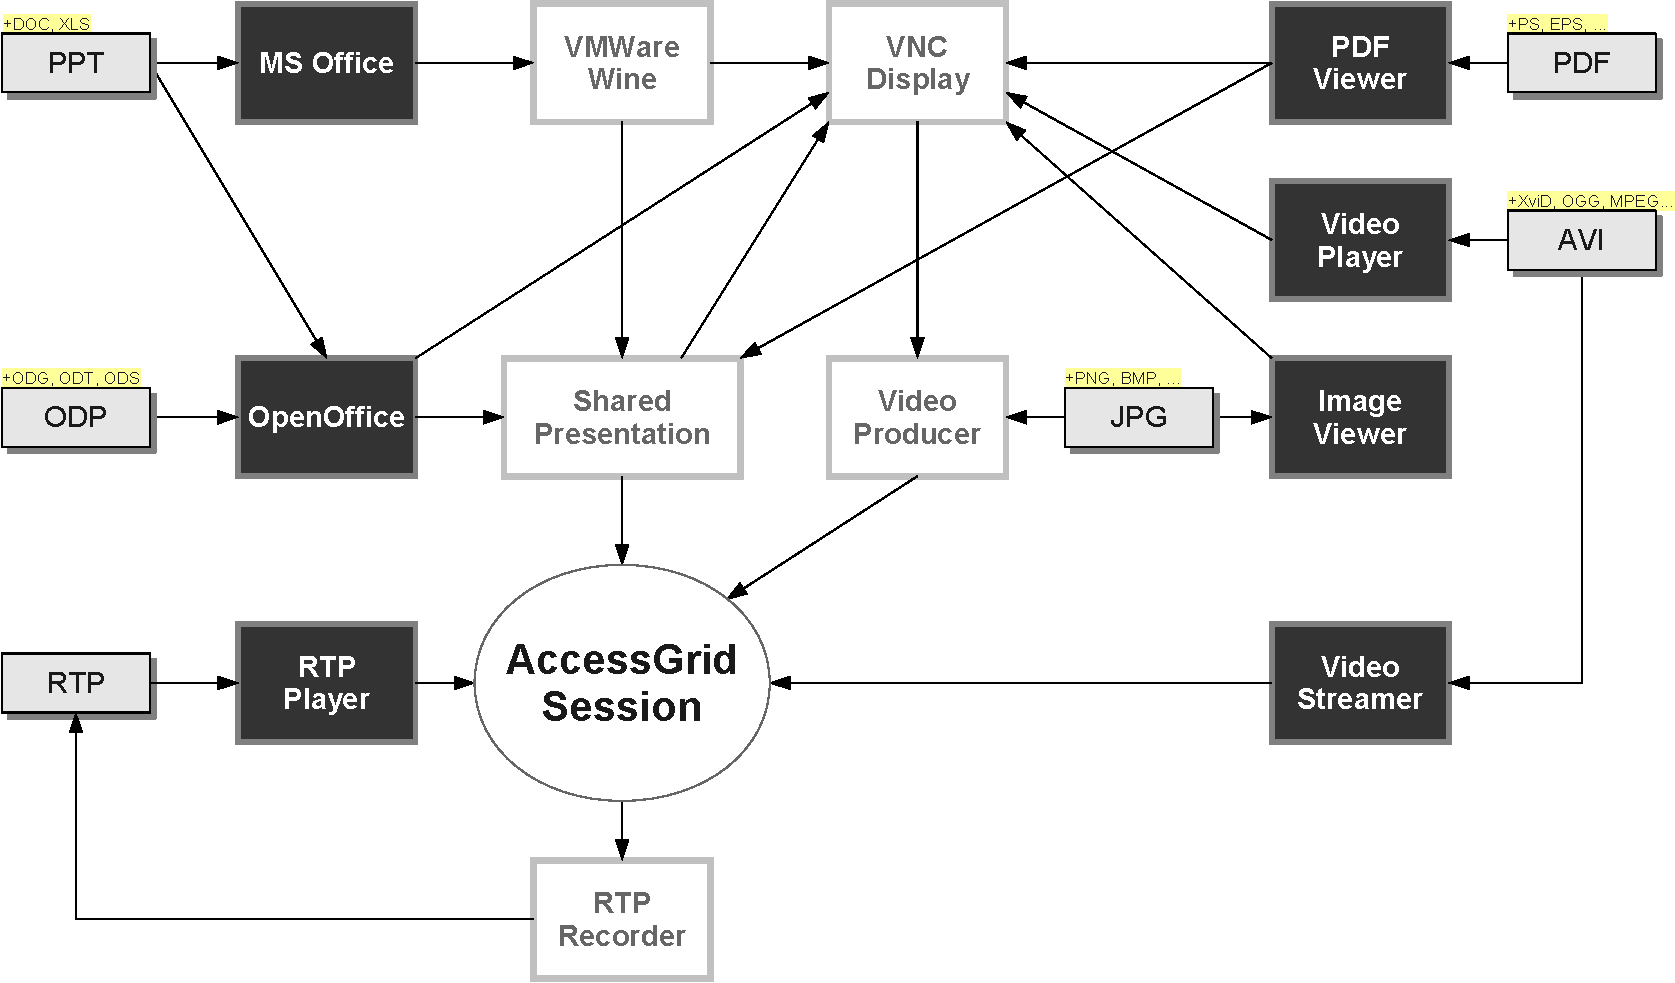
\includegraphics[width=1\textwidth]{images/vc-input-formats}
\caption{Využitie rôznych formátov v~prezentácii.}
\label{fig:PresentationFileFormats}
\end{figure}

Len pre úplnosť uvádzame, že existuje ešte robustnejší protokol pôvodom z~Microsoft Terminal Services s~názvom \textbf{RDP ITU T.128}, ktorý prenáša aj zvuk, súbory a zdieľané disky. V~tejto práci však budeme používať jednoduchší systém VNC.


\subsection{Shared presentations}
Linuxová verzia AG 2.4 obsahuje nástroje SharedBrowser, SharedPresentation a SharedPDF. \textbf{SharedPresentation} používa OpenOffcie pre zobrazovanie prezentácií vo formáte PPT (MS PowerPoint), ODP (Open Document Presentation) a SXI (Staršia verzia OpenOffice/StarOffice). \textbf{SharedPDF} umožňuje zdieľať prezentácie uložené vo~formáte PDF a pod Linuxom využíva aplikáciu xpdf. \textbf{SharedBrowser} využíva internetový prehliadač Mozilla.

Užívateľ iste narazí na niekoľko nepríjemných chýb (alebo vlastností?) týchto aplikácií. V~prípade SharedPDF sa zobrazujú vždy dve rovnaké okná s~PDF dokumentom, pričom by stačilo len jedno. Využitie by iste našla aj podpora pre prehliadač KPDF. V~prípade SharedBrowser musí byť ručne doinštalovaný modul pre Python, ktorý vytvorí rozhranie pre prehliadač Mozilla, inak aplikácia nefunguje. Navyše chýba podpora pre prehliadače Konqueror a Opera. SharedPresentation zas neumožňuje ovládanie fullscreen prezentácie a chýba filter pre súbory s~príponou ODP. Opravenú verziu ponúkame záujemcom na stránkach projektu Ciant AG node \cite{CIANT-AGnodeWiki}.

\subsection{Shared desktop}
AccessGrid tiež obsahuje dva VNC nástroje -- starší VenueVNC a jeho nástupcu SharedDektop \cite{AG-SharedDesktop}. Zdieľanú pracovnú plochu je možné využiť nielen pri prezentáciách ale aj ako nástroj pri riešení technických problémov.

Zaujímavý projekt sľubujú stránky Vislabu, ktoré popisujú aplikáciu SharedDesktop \cite{Vislab-SharedDesktop}. Zmenou oproti klasickému VNC je prenos zvuku, 3D akcelerácia a zobrazovanie kurzorov myši všetkých pripojených klientov. Vývoj tejto aplikácie však postupuje veľmi pomaly a zatiaľ neexistuje žiadna použiteľná verzia.

\subsection{Shared media player}
Aplikácia Shared Media Player bola zatiaľ doménou výlučne operačného systému Windows \cite{AG-SharedMoviePlayer}. Rozhodli sme sa preto vytvoriť zdieľanú aplikáciu podobného typu aj pre systém Linux. Riešenie sa opiera o~schopnosti prehrávača MPlayer, ktorý je dostupný pre široké spektrum unixových operačných systémov a dokonca aj pre systém Windows. Pri tvorbe sme vychádzali z~aplikácie SharedPDF, ktorá umožňuje zdieľanú prezentáciu PDF dokumentov. Rozhranie k~xpdf sme nahradili rozhraním k~aplikácii MPlayer.

Inštalačný balík poskytujeme na wiki-stránkach projektu Ciant AG node \cite{CIANT-SharedMPlayer}. Inštalácia vyžaduje spustenie príkazu:
\begin{verbatim}
agpm.py -z SharedMPlayer.zip
\end{verbatim}

\subsection{Further shared applications}
Pre úplnosť by sme ešte radi spomenuli aplikáciu \textbf{SharedRasmol} \cite{AG-SharedRasmol}, ktorá umožňuje 3D vizualizáciu molekúl, \textbf{Shared Question Tool} \cite{AG-SharedQuestionTool} pre zdieľanú tvorbu otázok a odpovedí a \textbf{AGBasicImage}, ktorá umožňuje zdieľané prezeranie obrázkov a úpravu ich metadát.
Ďalej \textbf{Media Lecture Board}, ktorá umožňuje zdieľanú tvorbu dokumentov. V~praxi sa však ukázala ako veľmi nestabilná.

%%%%%%%%%%%%%%%%%%%%%%%%%%%%%%%%%%%%%%%%%%%%%%%%%%%%%%%%%%%%%%%%%%%%%
%%%%%%%%%%%%%%%%%%%%%%%%%%%%%%%%%%%%%%%%%%%%%%%%%%%%%%%%%%%%%%%%%%%%%
\section{G-Ware configuration tool}
%%%%%%%%%%%%%%%%%%%%%%%%%%%%%%%%%%%%%%%%%%%%%%%%%%%%%%%%%%%%%%%%%%%%%
%%%%%%%%%%%%%%%%%%%%%%%%%%%%%%%%%%%%%%%%%%%%%%%%%%%%%%%%%%%%%%%%%%%%%

Zariadenia na potlačenie spätnej väzby od firmy ClearOne (predtým Gentner) sa konfigurujú pomocou jednotného nástroja G-Ware.
AG uzol v~organizácii CIANT využíva verziu AP-800. Ešte donedávna bola situácia komplikovaná tým, že software existuje iba vo verzii pre operačný systém Windows. Aplikácia sa síce používa iba pri výrazných zásahoch do parametrov miestnosti, ale bolo nutné vlastniť aspoň jednu licenciu na inak nevyužívaný operačný systém. Najnovšie verzie Wine a CrossoverOffice však už bezproblémov dokážu tento nástroj emulovať v prostredí Linuxu (obrázok \ref{fig:GWareInWine}). Tým skončila posledná závislosť na OS Windows. Inštalačný balík G-Ware s~veľkosťou cca 20MiB je možné získať na stránkach výrobcu ClearOne \cite{ClearOne-ResourceLibrary} spolu so~všetkými potrebnými manuálmi.

Detailný popis inštalácie pre staršie verzie Wine poskytujú stránky Vislabu \cite{Vislab-GWare}, autori popisujú kompiláciu zo zdrojových kódov vrátane potrebného patch súboru.

\begin{figure}
\centering
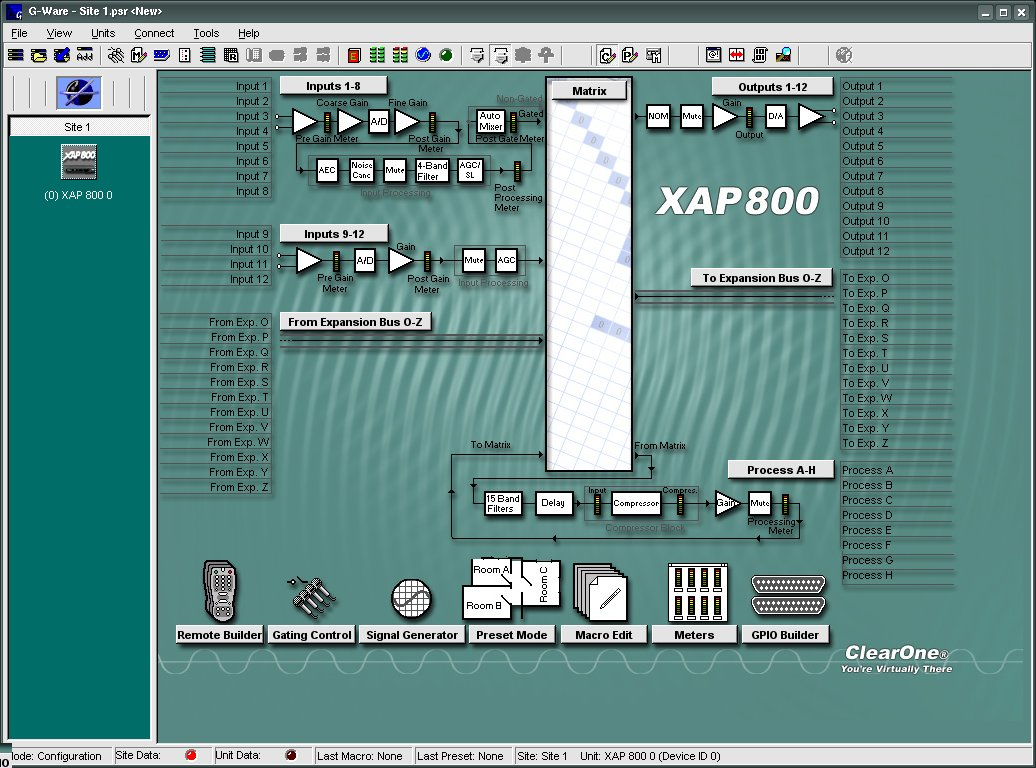
\includegraphics[width=0.9\textwidth]{images/gware}
\caption{G-Ware emulovaný pomocou Wine.}
\label{fig:GWareInWine}
\end{figure}

%%%%%%%%%%%%%%%%%%%%%%%%%%%%%%%%%%%%%%%%%%%%%%%%%%%%%%%%%%%%%%%%%%%%%
%%%%%%%%%%%%%%%%%%%%%%%%%%%%%%%%%%%%%%%%%%%%%%%%%%%%%%%%%%%%%%%%%%%%%
\section{Bridging the multicast}
%%%%%%%%%%%%%%%%%%%%%%%%%%%%%%%%%%%%%%%%%%%%%%%%%%%%%%%%%%%%%%%%%%%%%
%%%%%%%%%%%%%%%%%%%%%%%%%%%%%%%%%%%%%%%%%%%%%%%%%%%%%%%%%%%%%%%%%%%%%

Architektúra AccessGridu je do veľkej miery závislá na multicastovom pripojení. Jeho správne fungovanie sa overuje pomocou nástroja Multicast Beacon. Môže však nastať situácia, kedy niektorý z~uzlov dočasne alebo permanentne nepodporuje multicast. Problémy spojené s~dostupnosťou muticastu je možné rozdeliť na 3 skupiny:

\begin{enumerate}
\item Sieť bez podpory multicastu.
\item Vznik izolovaných multicastových oblastí.
\item Problémy spojené s~prechodom cez NAT a firewall.
\end{enumerate}

V~historii AccessGridu sa objavilo niekoľko pokusov o~prekonanie týchto problémov. Vznikli tak projekty RCBridge, QuickBridge, AGConnector a komerčný InSORS Enterprise Manager.

\paragraph*{RCBridge:}
Je nástroj napísaný v~jazyku Java s~webovým rozhraním, ktorý forwarduje pakety medzi multicastovou a unicastovou sieťou. Nástroj však nie je integrovaný s~architektúrou AccessGridu.

\paragraph*{QuickBridge:}
Je jednoduchý UDP forwarder napísaný v~jazyku C, ktorý je dodávaný ako súčasť inštalačného balíka AccessGridu 2.4. Nevýhodou je neúspech pri prekonávaní NAT.

\paragraph*{AGConnector:}
Riešenie založené na myšlienke tunelovania multicastových paketov pomocou jedného UDP spojenia. Obsahuje dva hlavné komponenty -- UMTP Agent a UMTP Server. Táto aplikácia existuje len pre AccessGrid 3.0.

\paragraph*{InSORS Enterprise Manager:}
Komerčné riešenie, ktoré okrem multicastového mostu ponúka navyše H.323 bridge a IG Pix Presentation Server pre nahrávanie zdieľaných prezentácií.


\subsection{QuickBridge}

Funkcia komponentu QuickBridge je znázornená na obrázku \ref{fig:QuickBridge}. Aplikácia preposiela pakety medzi multicastovou sieťou a unicastovými uzlami použité UDP porty je možné ľubovolne nastavovať. Detailná dokumentácia, popis inštalácie a zdrojové kódy sa nachádzajú na stránkach projektu AccessGrid \cite{AG-BridgingGuide}.

Pre zjednodušenie si predstavme nasledujúcu situáciu: Všetky uzly odosielajú a prijímajú UDP pakety na multicastovej adrese 224.0.0.1 na porte 10000. Jedným z~uzlov je aj QuickBridge, ktorý navyše akceptuje unicastové spojenia vo forme UDP paketov na porte 20000. QuickBridge si vedie zoznam aktívnych uzlov, ktoré mu poslali UDP pakety na tento port. Každý UDP paket z~unicastovej siete preposiela do multicastovej siete a naopak. Pokiaľ unicastový uzol po istú dobu neodpovedá, QuickBridge ho vyškrtne zo zoznamu a už mu nepreposiela nové pakety. Takúto jednoduchú situáciu môžeme namodelovať príkazom:
\begin{verbatim}
QuickBridge -g 224.0.0.1 -m 10000 -u 20000
\end{verbatim}

V~prostredí AccessGridu sa QuickBridge konfiguruje vždy pre nejaký VenueServer a to pomocou konfiguračného súboru \textbf{BridgeServer.cfg}. Ako príklad konfigurácie môžeme uviesť existujúce nastavenie pre uzol v~organizácii CIANT, ktorý sme popisovali v~kapitole \ref{kap:CIANT-AG-Bridge}. Bridge je potom možné spustiť príkazom:
\begin{verbatim}
BridgeServer.py -c ./BridgeServer.cfg
\end{verbatim}

\begin{verbatim}
# BridgeServer.cfg
[BridgeServer]
name = CiantMagicUnicastBridge
location = Prague
qbexec = /usr/bin/QuickBridge
BRIDGESERVER = CiantMagicUnicastBridge
\end{verbatim}

\begin{verbatim}
# Use this port range for the bridge server as a whole
portMin = 20000
portMax = 20005
\end{verbatim}

\begin{verbatim}
# Name of Lobby that you wish to provide a bridge to
[https://195.113.187.114:8000/Venues/default]
type = Venue
\end{verbatim}

\begin{figure}
\centering
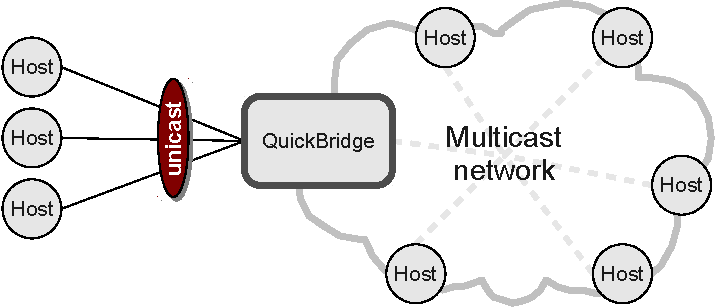
\includegraphics[width=0.7\textwidth]{images/arch-quickbridge}
\caption{Premostenie multicastu pomocou QuickBridge.}
\label{fig:QuickBridge}
\end{figure}

Problém použitia QuickBridge v~prostredí s~NAT spočíva vo vlastnosti  protokolov RTP/RTCP. Pre jedno dátové spojenie sa používajú vždy dva UDP porty -- $2k$ pre RTP a $2k+1$ pre RTCP. Cez NAT tak prejde RTCP informácia ale opačným smerom už RTP neprejde.

\subsection{AGConnector}
Tento software nahradzuje QuickBridge v~novej verzii AccessGridu (verzia 3.0). Rieši problém prenosu multicastových paketov medzi multicastovými ostrovmi, špeciálne prípad siete za firewallom a NATom. AGConnector využíva protokol UMTP \ref{kap:UMTP}, pomocou ktorého tuneluje multicastové UDP pakety medzi multicastovými ostrovmi (obrázok \ref{fig:AGConnector}). Prenos zabezpečuje jediný UDP port 8010 UDP, ktorý nesmie byť blokovaný firewallom. Inštalácia prebieha príkazom:
\begin{verbatim}
agpm.py –z AG_Connector.zip
\end{verbatim}

\begin{figure}
\centering
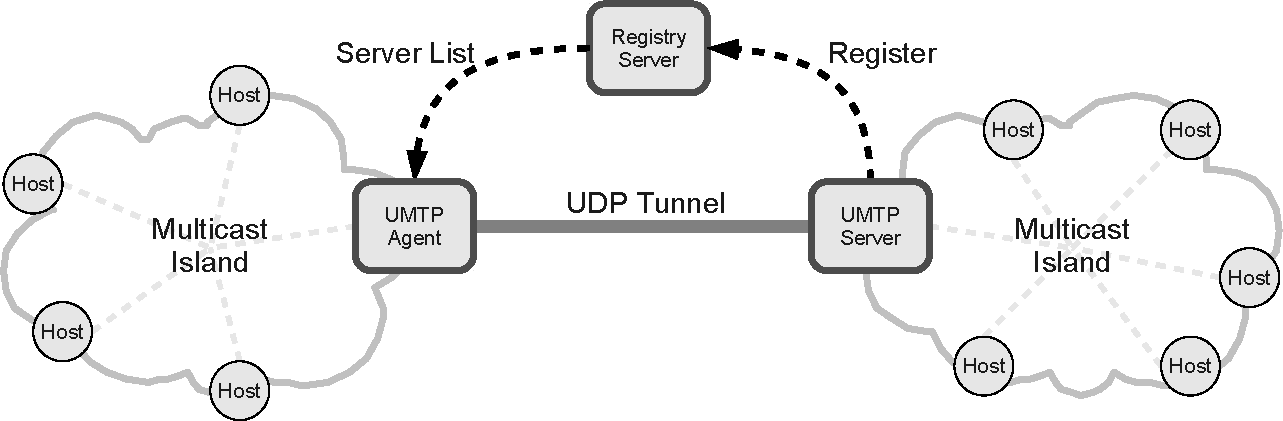
\includegraphics[width=1\textwidth]{images/arch-agconnector}
\caption{Premostenie multicastu pomocou AGConnector. (zdroj \protect\cite{AG-Connector})}
\label{fig:AGConnector}
\end{figure}

%%%%%%%%%%%%%%%%%%%%%%%%%%%%%%%%%%%%%%%%%%%%%%%%%%%%%%%%%%%%%%%%%%%%%
%%%%%%%%%%%%%%%%%%%%%%%%%%%%%%%%%%%%%%%%%%%%%%%%%%%%%%%%%%%%%%%%%%%%%
\section{Results and suggestions}
%%%%%%%%%%%%%%%%%%%%%%%%%%%%%%%%%%%%%%%%%%%%%%%%%%%%%%%%%%%%%%%%%%%%%
%%%%%%%%%%%%%%%%%%%%%%%%%%%%%%%%%%%%%%%%%%%%%%%%%%%%%%%%%%%%%%%%%%%%%
Všetky komponenty potrebné pre chod plnohodnotného AccessGridového uzla je možné prevádzkovať v~operačnom systéme Linux. Problémovými aplikáciami boli G-Ware a SharedMediaPlayer. V~rámci tejto práce sme vytvorili zdieľanú aplikáciu SharedMPlayer, ktorá poskytuje podobné funkcie ako SharedMediaPlayer pre Windows. Navyše ťažíme z~obrovského množstva kodekov, ktoré podporuje MPlayer. Ostatné zdieľané aplikácie, ktoré sme popisovali, existujú pre obe platformy. G-Ware je možné emulovať v~prostredí Wine.

Stav videokonferenčného uzla je potrebné preventívne testovať. Pre tento účel usporiadava komunita AG pravidelné stretnutia zameraná na odhaľovanie a odstraňovanie problémov za pomoci skúsených užívateľov AG. Užitočné informácie o~odstraňovaní problémov so zvukom, obrazom, sieťovým pripojením a zdieľanými aplikáciami sa nachádzajú priamo na stránkach AG \cite{AG-QualityAssurancePreparation}.

\proofed

		%%%%%%%%%%%%%%%%%%%%%%%%%%%%%%%%%%%%%%%%%%%%%%%%%%%%%%%%%%%%%%%%%%%%%
%%%%%%%%%%%%%%%%%%%%%%%%%%%%%%%%%%%%%%%%%%%%%%%%%%%%%%%%%%%%%%%%%%%%%
%%%%%%%%%%%%%%%%%%%%%%%%%%%%%%%%%%%%%%%%%%%%%%%%%%%%%%%%%%%%%%%%%%%%%
%%%%%%%%%%%%%%%%%%%%%%%%%%%%%%%%%%%%%%%%%%%%%%%%%%%%%%%%%%%%%%%%%%%%%
\chapter{Recording the conference}
%%%%%%%%%%%%%%%%%%%%%%%%%%%%%%%%%%%%%%%%%%%%%%%%%%%%%%%%%%%%%%%%%%%%%
%%%%%%%%%%%%%%%%%%%%%%%%%%%%%%%%%%%%%%%%%%%%%%%%%%%%%%%%%%%%%%%%%%%%%
%%%%%%%%%%%%%%%%%%%%%%%%%%%%%%%%%%%%%%%%%%%%%%%%%%%%%%%%%%%%%%%%%%%%%
%%%%%%%%%%%%%%%%%%%%%%%%%%%%%%%%%%%%%%%%%%%%%%%%%%%%%%%%%%%%%%%%%%%%%

%%%%%%%%%%%%%%%%%%%%%%%%%%%%%%%%%%%%%%%%%%%%%%%%%%%%%%%%%%%%%%%%%%%%%
%%%%%%%%%%%%%%%%%%%%%%%%%%%%%%%%%%%%%%%%%%%%%%%%%%%%%%%%%%%%%%%%%%%%%
\section{Recording vs. archiving}
%%%%%%%%%%%%%%%%%%%%%%%%%%%%%%%%%%%%%%%%%%%%%%%%%%%%%%%%%%%%%%%%%%%%%
%%%%%%%%%%%%%%%%%%%%%%%%%%%%%%%%%%%%%%%%%%%%%%%%%%%%%%%%%%%%%%%%%%%%%

At the beginning of this chapter, we distinguish between recording and archiving. The purpose of recording is to create a record that can later be reconstructed. Archiving additionally takes into account the overall context in which the record was created. We would like to emphasise this distinction in connection with the OAIS reference model \cite{OAIS-RM}, an ISO standard that provides a framework for long-term preservation. This rather extensive standard can be summarised by a simple, recursive idea:

\begin{quote}
Archiving data requires archiving the metadata and the tools needed to interpret that data. This process is repeated recursively, extending as far as the archival description of the protocols and encodings used.
\end{quote}

It is clear that archiving favours open technologies based on open standards over closed, undocumented systems. This leads us as far as the source code itself. Such an approach ensures that archived data can be reconstructed even several decades later.

A system based on freely available components is therefore the first step towards successful archiving. The remaining task is to address the recording process itself, define which aspects of communication should be archived, and select suitable tools.

%%%%%%%%%%%%%%%%%%%%%%%%%%%%%%%%%%%%%%%%%%%%%%%%%%%%%%%%%%%%%%%%%%%%%
%%%%%%%%%%%%%%%%%%%%%%%%%%%%%%%%%%%%%%%%%%%%%%%%%%%%%%%%%%%%%%%%%%%%%
\section{Data streams within an AccessGrid session}
%%%%%%%%%%%%%%%%%%%%%%%%%%%%%%%%%%%%%%%%%%%%%%%%%%%%%%%%%%%%%%%%%%%%%
%%%%%%%%%%%%%%%%%%%%%%%%%%%%%%%%%%%%%%%%%%%%%%%%%%%%%%%%%%%%%%%%%%%%%

AccessGrid consists of several interconnected components. Their communication can be divided into two main groups:
\begin{enumerate}
\item multimedia data transmission,
\item transmission of control messages.
\end{enumerate}

In Chapter \ref{kap:Multicast}, we described multicast as one of the delivery methods. It is particularly suitable for multimedia data in group communication. The RTP protocol is used for the actual transmission.

Control messages, on the other hand, account for only a small part of the overall communication and are therefore transmitted using the simpler unicast method. More specifically, communication between the VenueServer and the other AccessGrid components takes place in a form of XML-RPC.

\subsection{Candidates for archiving}

The most suitable candidates for recording, archiving and subsequent reconstruction are multimedia streams -- audio and video. The next candidates are the presentation display and, further, the desktop. Control messages and various message fragments related to security are less suitable candidates.

% In practice, it makes sense to record only streams that do not depend on state information. Successful recording would require state reconstruction, which may encounter limits of spatial and temporal complexity, and even computability in theoretical extremes.

Audio and video signals are essentially stateless. Codecs that generate transitions between keyframes rather than encoding individual frames introduce some complications. In the worst case, this can be handled by skipping to the next keyframe. The same principle applies to data fragmentation at individual ISO/OSI layers. The point is that audio and video carried in RTP packets should be relatively easy to archive. When reconstructing a damaged recording, the most complicated task will be to find the next keyframe, which depends on the codec being used.

Another candidate is the RFB protocol used for communication between a VNC server and client. The protocol is stateless, and terminating the connection or experiencing connection outages does not compromise the consistency of a VNC session.

As already mentioned, AccessGrid uses XML-RPC to control its components. In general, this communication is not of particular interest to us, with one exception: XML-RPC is used to synchronise AccessGrid shared applications. A shared presentation is an especially promising candidate for recording. One possible solution would be to store slide-transition events using a specially modified version of SharedPresentation. The problem, however, is the development of a universal recording tool for all shared applications. Moreover, the stored information could only be replayed in the same way in which it was created. In the context of OAIS, we would also have to archive all the viewers and shared applications used.

\subsection{Conversion to a common format}

\begin{quote}
\ldots or how to avoid $n^2$ conversion tools while using only $n$ formats
\end{quote}

To simplify the archiving process as much as possible, we decided to convert all events occurring during a videoconference into an audiovisual format and store them as RTP packets. Conversion may slightly reduce the quality of the original data, but it provides a uniform format for which playback and editing tools can later be developed.

\paragraph*{VNC display:} Conversion requires capturing the desktop image and encoding it with a suitable codec into RTP format.

\paragraph*{Shared presentation:} It is sufficient to capture the part of the desktop that displays the presentation. We can reuse the previous approach and use VNC to display the presentation. This solution is not limited to presentations in PDF or ODP format.

\begin{figure}
\centering
\includesvg[width=0.6\textwidth]{oais-environment}
\caption{The OAIS archival environment \cite{OAIS-RM}.}
\label{fig:OaisEnvironment}
\end{figure}

The OAIS reference model defines four elements of an archival environment (Figure \ref{fig:OaisEnvironment}). From our perspective, the \textquotedblleft Producer\textquotedblright\ is any application that transmits RTP packets, namely VIC and RAT. The \textquotedblleft Consumer\textquotedblright\ is the user who wants to reconstruct and play back an archived recording, for example using VIC and RAT. To follow the reference model, we would also have to provide a \textquotedblleft Management\textquotedblright\ entity responsible for setting the policies followed by the OAIS archival environment. Archive maintenance is therefore not performed by management itself, but by structures within the archive.

Implementing the OAIS model is outside the scope of this thesis, and the remainder of this chapter is independent of the archival paradigm used.

%%%%%%%%%%%%%%%%%%%%%%%%%%%%%%%%%%%%%%%%%%%%%%%%%%%%%%%%%%%%%%%%%%%%%
%%%%%%%%%%%%%%%%%%%%%%%%%%%%%%%%%%%%%%%%%%%%%%%%%%%%%%%%%%%%%%%%%%%%%
\section{Existing recording tools}
%%%%%%%%%%%%%%%%%%%%%%%%%%%%%%%%%%%%%%%%%%%%%%%%%%%%%%%%%%%%%%%%%%%%%
%%%%%%%%%%%%%%%%%%%%%%%%%%%%%%%%%%%%%%%%%%%%%%%%%%%%%%%%%%%%%%%%%%%%%

\subsection{Tcpdump -- packet sniffer}
Tcpdump can save packets passing through a network interface. At first glance, it might seem to be an ideal tool for capturing all information in a data transmission. The problem with recording RTP packets, however, is preserving their timing. Although the resulting file contains all audiovisual data, reconstructing the original timing is difficult. Tcpdump is therefore not a suitable tool for this purpose.

\subsection{RTPtools}
RTPtools is a set of utilities for working with RTP streams. It includes rtprecord, rtpplay and rtpproxy. Another tool is the RTP reflector, which can mirror incoming data, mix different RTP streams and transparently transcode communication using another codec.
All these tools are command-line applications and provide only basic functionality.

\subsection{AGVCR -- RTP recorder/player}
At the time of writing, the most suitable tool for recording RTP packets is AGVCR by D. Piper \cite{AGVCR-home} of Indiana University. It provides both graphical and text-based interfaces (including Telnet), and supports automatic launching of applications used for recording and playing multimedia. The recording is stored in a separate file containing information about all received data streams and their timing. The tool also allows a subset of the recorded data to be exported by splitting it into smaller segments.

%%%%%%%%%%%%%%%%%%%%%%%%%%%%%%%%%%%%%%%%%%%%%%%%%%%%%%%%%%%%%%%%%%%%%
%%%%%%%%%%%%%%%%%%%%%%%%%%%%%%%%%%%%%%%%%%%%%%%%%%%%%%%%%%%%%%%%%%%%%
\section{Recording an ongoing conference}
%%%%%%%%%%%%%%%%%%%%%%%%%%%%%%%%%%%%%%%%%%%%%%%%%%%%%%%%%%%%%%%%%%%%%
%%%%%%%%%%%%%%%%%%%%%%%%%%%%%%%%%%%%%%%%%%%%%%%%%%%%%%%%%%%%%%%%%%%%%

The purpose of recording is to capture the course of a conference as faithfully as possible from the perspective of a single node. The simplest option, which we also used for the node at the Ciant organisation, is to record the signal from a graphics card, for example as an S-Video signal. The advantages and disadvantages of this solution were discussed in Chapter \ref{kap:CiantSkusenosti}.

A more complex approach uses AGVCR. Recording requires a dedicated computer because, within one operating system, it is not possible to record, view and transmit packets using the same socket at the same time. The last application to call \verb|bind()| receives the packets; the other applications can only transmit data using \verb|send()| or \verb|sendto()|.

For a large conference, the recording node must have sufficient processing power, disk space and a high-quality network connection. It stores all packets appearing in the conference. Fortunately, the node does not need to encode or decode any data streams; its only task is to store RTP packets.

%%%%%%%%%%%%%%%%%%%%%%%%%%%%%%%%%%%%%%%%%%%%%%%%%%%%%%%%%%%%%%%%%%%%%
%%%%%%%%%%%%%%%%%%%%%%%%%%%%%%%%%%%%%%%%%%%%%%%%%%%%%%%%%%%%%%%%%%%%%
\section{StreamVNC -- a new tool for local recording}
%%%%%%%%%%%%%%%%%%%%%%%%%%%%%%%%%%%%%%%%%%%%%%%%%%%%%%%%%%%%%%%%%%%%%
%%%%%%%%%%%%%%%%%%%%%%%%%%%%%%%%%%%%%%%%%%%%%%%%%%%%%%%%%%%%%%%%%%%%%

The problem of conference recording led to the idea of creating a tool that would allow a presentation to be prepared by transmitting it to a local network interface -- localhost. During the design of the system, we considered the following requirements:
\begin{paklist}
\item Simple operation.
\item A graphical user interface.
\item The ability to record the desktop, for example while a presentation is running.
\item Sufficient recording quality.
\item Low network bandwidth requirements.
\item Support for both audio and video recording.
\item Reuse of existing components.
\item Easy editing (cutting) of the resulting recording.
\item Simple playback.
\end{paklist}

The first problem was finding suitable components that could communicate with one another and were sufficiently configurable and controllable. They had to cover the following areas:
\begin{paklist}
\item Recording RTP packets.
\item Audio processing.
\item Capturing and processing camera video.
\item Capturing and processing the desktop image.
\item Providing suitable presentation tools.
\end{paklist}

The model situation is shown in Figure \ref{fig:LocalhostRecording}. The key element is the VNC system (1), which can display an application (2) independently of the surrounding desktop. The figure shows the VNC content being sent to a local address by the VIC application (3), together with audio from RAT (4) and an additional camera video stream (5). All three data streams are recorded by AGVCR (6).

\begin{figure}
\centering
\includesvg[width=0.8\textwidth]{localhost-recording}
\caption{Preparing a presentation for later use.}
\label{fig:LocalhostRecording}
\end{figure}

\subsection{Recording RTP packets}
The excellent AGVCR tool simplified the selection of a suitable recording application. It required no further modifications because it was highly stable, efficient and configurable. The only missing feature was the ability to cut a segment from a saved recording. At the time of writing, we had already submitted this feature request to the application author.

\subsection{Audio processing}\label{kap:HybridRAT}
Before use, we had to make minor modifications to the RAT application, which transmits audio using RTP packets. The standard RAT 4.3 version from UCL had a problem when a firewall was enabled. The application refused to start, which was unacceptable for our purposes. The cause was communication by the \textquotedblleft mbus\textquotedblright\ component used by RAT. At startup, it always attempted to contact one of the multicast addresses, causing the application to freeze when a firewall was running. After some time, we found another modified version of RAT from VRVS, which started without problems.

Its disadvantage was the lack of an interface for ALSA (Advanced Linux Sound Architecture). It supported only OSS (Open Sound System), which had poor performance and problems interacting with other applications using audio. We therefore used the source code of both implementations to create a hybrid version, RAT-SVNC, combining the advantages of each.

\subsection{Desktop video processing}
Within AccessGrid, the VIC application is used to process video signals. Again, we could not use the original version from UCL. The application locks the socket on which it transmits RTP packets, preventing AGVCR from recording them. It also includes a poorly functioning H.263 codec, whose use often causes a \textquotedblleft segmentation fault\textquotedblright\ error. The VRVS version of VIC, based on the OpenMash project, contained a working H.263 codec and had a more compact design, which is particularly important for end users. In the EVO project, we also found a newer version of VIC called Vievo. We liked its design and decided to use it as the basis for the new tool.

We chose the name EVIC for the new version of VIC. It contains the core from the OpenMash-based VIC-VRVS and parts of the Vievo design. We added controls that allow recording to be controlled from an external X11 display. We use this feature when recording VNC content, allowing the controls to be placed on the physical X11 display.

The performance of the OpenMash VIC allows us to achieve 2 fps at PAL resolution and 10 fps at CIF resolution. These values are sufficient for presentation purposes and also save network bandwidth. Nevertheless, the performance of this component should be improved in the future. Tests showed that 8 fps at PAL resolution used 100\% of the processing capacity of a 1.8 GHz Pentium 4 processor.

\subsection{Camera video processing}

We also successfully used VIC to capture camera video at 25 fps and CIF resolution. PAL resolution is not yet supported. Camera video is intended as supplementary information accompanying the more important presentation and audio.

\subsection{Support for presentation tools}

When selecting presentation tools, we focused primarily on support for PDF, OpenDocument Format (ODF) and PowerPoint (PPT). We also wanted an image viewer, web-page presentation, limited support for video sequences and support for the VMware virtual machine. Extensibility to additional applications was also essential. The version of TightVNC we use does not support 3D acceleration, so applications using OpenGL are not supported yet.

In addition to the application itself, the VNC display required a suitable window manager. Important selection criteria included its size, resource requirements and the placement of window decorations. We eventually selected FLWM, which places window decorations on the left side. This avoids visual conflicts with the decorations of the VNC viewer. Before using it, we made minor modifications to FLWM, including adding the \verb|-e| parameter, which allows another program to be started when FLWM launches. For example, this allows us to set the desktop background using the command \verb|xsetroot -solid '#004455'|.

\subsection{StreamVNC architecture}

All components mentioned above were integrated into a single system, StreamVNC, shown in Figure \ref{fig:ArchStreamVNC}.

The system offers a high degree of configurability while requiring very little from the user. It uses C, TCL/Tk and shell script. It requires a running X server, on which all controls are displayed. The main architectural components are:
\begin{paklist}
\item RTP packet recording,
\item audio capture,
\item VNC -- server, viewer and desktop capture,
\item camera video capture,
\item applications.
\end{paklist}

\begin{figure}
\centering
\includesvg[width=1\textwidth]{arch-stream-vnc}
\caption{StreamVNC system architecture.}
\label{fig:ArchStreamVNC}
\end{figure}

Using Xvnc (the TightVNC server) requires the \verb|fixed| and \verb|helvetica| fonts. The font path is usually configured correctly by the Linux distribution, as is the case with OpenSUSE. Some distributions, such as Gentoo, require the font path to be set explicitly using \verb|Xvnc -fp <dir>|. StreamVNC therefore provides a binary version of Xvnc together with the essential fonts and the \verb|fonts.dir| and \verb|fonts.alias| definitions. The Xvnc server is not started directly, but through the \verb|vnc/Xvnc-run| script, which sets the custom font path. If necessary, this script can simply be modified.

\subsection{Implemented profiles}
The main script, \verb|agvcr-run|, is started either without parameters or with one parameter specifying the name of the file to be played. The application therefore distinguishes two profiles using separate configuration files: recording uses \verb|.agvcr.conf|, while playback uses \verb|.play.conf|.

\paragraph*{Recording profile:} This is the default profile, intended for recording a presentation. Programs shown in grey in Figure \ref{fig:SequenceStreamVNC} are started only in this profile. The user is presented with a menu from which one of the applications can be selected.

\paragraph*{Playback profile:}
In this profile, AGVCR automatically transmits RTP packets from the file supplied as its parameter. Only one instance of EVIC is started, after it receives an RTCP packet. The VNC server and VNC viewer are not started because they would unnecessarily occupy screen space during playback. The transmitted RTP packets are automatically received by RAT and EVIC, and the user sees the content of the saved presentation.

\begin{figure}
\centering
\includesvg[width=1\textwidth]{sequence-stream-vnc}
\caption{Dependencies between programs started by StreamVNC.}
\label{fig:SequenceStreamVNC}
\end{figure}

\subsection{Managing running processes}
Since this is an integrated system consisting of many communicating processes, process management was one of the most important issues. The main executable, called \verb|stream-vnc|, is implemented as a shell script. Its task is to start child processes, monitor their activity and terminate them all when necessary. The main obstacle was the limited flexibility of shell job control\footnote{Specifically, GNU bash version 3.00.16(1)-release (i586-suse-linux).}. We eventually solved the problem as follows:

The main program maintains a list of processes, \verb|$REQ|, whose termination should cause the entire system to shut down. It registers a signal handler for \verb|SIGCHLD|. When a child process terminates, the operating system kernel automatically notifies the parent process (signal 17). The shell uses the \verb|jobs -pr| command to obtain the list of running child processes. If a process from the \verb|$REQ| list is missing, the shutdown sequence is started and the parent sends \verb|SIGTERM| to the remaining child processes. In addition, all processes using the VNC display are automatically terminated when the VNC server exits.

Another approach we attempted to implement used the terminal functionality provided by the operating system. A terminal is a special device intended for inter-process communication. The operating system provides system calls for creating and managing this device. The process that creates the device becomes the leader of the process group that communicates through it. The group is identified by its process-group ID, which is the PID of its leader. If the leader terminates, the operating system should send the \verb|SIGHUP| signal to all processes in the group. The advantage is automatic signal delivery, unlike our application-level solution in the shell script.

The disadvantage is that some versions of shell interpreters do not provide equivalents of the \verb|grantpt()|, \verb|unlockpt()| and \verb|ptsname()| system calls. This must be handled by a small C program. It opens the special file \verb|/dev/ptmx|, which creates the master side of the communication channel. The Unix API provides the functions \verb|posix_openpt()|, \verb|grantpt(master)|, \verb|unlockpt(master)| and \verb|ptsname(master)|. The last function returns the name of a file such as \verb|/dev/pts/X|, where \verb|X| represents the slave side of the communication channel. A simple program therefore opens a pseudo-terminal, sets its file descriptors correctly, calls \verb|setsid()| to create a new session and process group, and becomes the leader of that group. It can then call one of the \verb|exec()| functions to start another process in its address space. Practical experience with StreamVNC showed, however, that the mechanism we selected is sufficient.

\subsection{Environment consistency check}
To make it easier to identify problems caused by missing applications, we added the \verb|--check| parameter to the \verb|stream-vnc| script. Before the first use, it is therefore advisable to run \verb|./stream-vnc --check|. This checks the consistency of the system and identifies the most common problems. Among other things, it also detects whether the operating system kernel's \verb|vmmon| module for VMware support is running.

\proofed

\begin{comment}

%%%%%%%%%%%%%%%%%%%%%%%%%%%%%%%%%%%%%%%%%%%%%%%%%%%%%%%%%%%%%%%%%%%%%
%%%%%%%%%%%%%%%%%%%%%%%%%%%%%%%%%%%%%%%%%%%%%%%%%%%%%%%%%%%%%%%%%%%%%
\section{Processing archived content}
%%%%%%%%%%%%%%%%%%%%%%%%%%%%%%%%%%%%%%%%%%%%%%%%%%%%%%%%%%%%%%%%%%%%%
%%%%%%%%%%%%%%%%%%%%%%%%%%%%%%%%%%%%%%%%%%%%%%%%%%%%%%%%%%%%%%%%%%%%%

How to overlay an image on a video:
http://www.videolan.org/doc/play-howto/en/ch04.html
\begin{verbatim}
vlc test.ogm --sub-filter logo --logo-file logo.png --logo-x 20 --logo-y 20
\end{verbatim}

Real-time transcoding to MPEG-4 video (128 kb/s) and OGG audio (32 kb/s):
\begin{verbatim}
vlc -vvv test.ogg --sout '#transcode{vcodec=mp4v, acodec=vorbis,vb=128,ab=32,deinterlace}:display'
\end{verbatim}

Various filters are described at:
http://www.videolan.org/doc/streaming-howto/en/ch03.html

2xPIP

\begin{verbatim}
vlc -vvv test.ogg --sout '#duplicate{
dst={transcode{vcodec=mp2v,vb=4096,scale=1,sfilter=mosaic}:bridge-in{offset=100}:display},
dst={duplicate{dst=mosaic-bridge{id=1,width=320,height=200},dst=mosaic-bridge{id=2,width=320,height=200}}}}'
\end{verbatim}

\begin{verbatim}
vlc --color -I telnet --vlm-conf /dev/shm/mosaic.conf --fake-file background.jpg
--fake-aspect-ratio "4:3" --mosaic-width 640 --mosaic-height 400 --mosaic-keep-picture --mosaic-rows 2 --mosaic-cols 2 --mosaic-position 1 --mosaic-order 1,2,3

MPlayer V4L loopback device
http://lists.mplayerhq.hu/pipermail/mplayer-dev-eng/
001-November/002600.html

vloopback
http://www.lavrsen.dk/twiki/bin/view/Motion/
VideoFourLinuxLoopbackDevice

VJ software that supports vloopback input/output:
http://www.gephex.org/

##################################
## HTTP interface mosaic wizard ##
##################################

# Comment out the following line if you do not want to reset the VLM configuration
del all

# Background options
new   bg broadcast enabled
setup bg input     "fake:" option "fake-file=background.jpg" option "fake-width=640" option "fake-height=400" option "fake-ar=4:3"
setup bg output\
	#transcode{vcodec=mp2v,vb=4096,scale=1,sfilter=mosaic}:\
	bridge-in{offset=100}:

# Mosaic options
setup bg option mosaic-alpha=200
setup bg option mosaic-height=400
setup bg option mosaic-width=640
setup bg option mosaic-align=5
setup bg option mosaic-xoffset=10
setup bg option mosaic-yoffset=10
setup bg option mosaic-vborder=5
setup bg option mosaic-hborder=10
setup bg option mosaic-position=1
setup bg option mosaic-rows=2
setup bg option mosaic-cols=2
setup bg option mosaic-order=1,2,3
setup bg option mosaic-delay=0
setup bg option mosaic-keep-picture

new channel1 broadcast enabled
setup channel1 input "test.ogg"
setup channel1 output \
	#mosaic-bridge{id=1,width=320,height=200},\
	select=audio,\
	dst=bridge-out{id=3},\
	select=audio

new channel2 broadcast enabled
setup channel2 input "test.ogg"
setup channel2 output \
	#duplicate{
		dst=mosaic-bridge{id=2,width=320,height=200},\
		select=video,\
		dst=bridge-out{id=3},\
		select=audio\
	}

# Input options
# Launch everything

control bg play
control channel1 play
control channel2 play

# end of mosaic batch
\end{verbatim}

RTSP is a text-based protocol similar to HTTP that could be used for media streaming. LIVE555 is a library that could provide this functionality.
Presentations could be stored in an appropriate format and played on demand by a server. Several solutions already exist, such as FFmpeg, Helix DNA and VLC.

An unresolved problem is transcoding RTP streams stored in the rtpplay format. The AGVCR format has the same problem. Ideally, we would need a utility that separates these streams into individual files according to their SSRC. We would then need another utility to convert each file into a suitable format that could be processed by mencoder or FFmpeg. VLC could then be used to create a grid containing several such streams.

The VRVS semester project indicates that XviD is suitable for archiving, but that no method was found for playing back a recorded RTP stream.

The thesis DP2006Patoraj.pdf describes JRAT, which is faster than RAT. It is written in Java but consumes somewhat more memory.

The thesis DP2006Svrcek.pdf describes an attempt to modify VIC so that it stores the stream in a file in YUV format, which is then compressed to XviD.

The following configuration was intended to record directly from VIC using MPlayer, but it did not work correctly. In theory, the procedure should be as follows:
Create an SDP file named test.sdp:
\begin{verbatim}
c=IN IP4 127.0.0.1
m=video 10000 RTP/AVP 31
\end{verbatim}

Then run mencoder with \verb|-ovc [raw|lavc|copy]| and \verb|sdp://test.sdp|, or try MPlayer instead of mencoder.

Next, start \verb|vic 127.0.0.1/10000|. The video appears in MPlayer, but with artefacts, and the log contains errors such as:
\begin{verbatim}
Error while decoding frame!
[h261 @ 0x8861b78]Bad picture start code
[h261 @ 0x8861b78]header damaged
Error while decoding frame!
[h261 @ 0x8861b78]Bad picture start code
[h261 @ 0x8861b78]header damaged
Error while decoding frame!
[h261 @ 0x8861b78]run overflow at 15x5
[h261 @ 0x8861b78]Error at MB: 130
\end{verbatim}

Conclusion: this approach does not work. VLC and FFmpeg exhibit the same problem.

\end{comment}

		\chapter{Conclusion}

The objectives set out in the introduction have been successfully achieved. We found a way to create a videoconferencing node based entirely on freely available components. The tools developed during this work make it possible to prepare and record a conference. The way in which we combined the existing components is unique within the Access Grid environment.

\paragraph*{We consider the following to be the main contributions:}
\begin{enumerate}
%---------------------------
\item Creation of a videoconferencing node at the Ciant organization. It is the second Access Grid node in the Czech Republic and can serve as a model for nodes at other organizations.

%---------------------------
\item As part of creating the node, a website was developed. In addition to information about the node itself, it contains a collection of tools related to videoconferencing technologies. The engine used to create the website is available to interested users.

%---------------------------
\item The contacts established through the node's activities to date will be used in future cooperation between MFF UK and the MARCEL network. This cooperation could generate further interesting projects that could serve as topics for bachelor's, master's, and doctoral theses.

%---------------------------
\item The practical experience gained while creating the node made it possible to design an Access Grid node composed entirely of freely available components. Applications that are otherwise available on commercial platforms had to be provided separately.

%---------------------------
\item Creation of a shared multimedia player for the Linux operating system—SharedMPlayer—which had previously been missing from Access Grid. The repair of the existing version of SharedPresentation is also worth mentioning.

%---------------------------
\item Another software component developed as a result of this work is EVIC, a modified version of the VIC application from the VRVS project. The main objective was to find a suitable candidate for recording a VNC screen, which the original VIC developed at UCL did not support. EVIC became part of the StreamVNC tool and provides control elements located on a remote X11 display.

%---------------------------
\item The integrated StreamVNC tool was developed to prepare presentations suitable for broadcasting to an Access Grid conference. It enables local recording of VNC content, audio, and video from a camera. The data stream, in the form of RTP packets, is stored using the AGVCR tool.

%---------------------------
\item From a theoretical perspective, we described the main problems of Access Grid and videoconferencing technologies in general. Using small examples, we demonstrated ways to traverse NAT and firewalls, as well as tunnelling and multicast-network bridging. For the node at Ciant, we built QuickBridge, which partially addresses the problem of multicast-network unavailability. In the future, we are considering deploying the newer version AG 3, which provides improved bridging using UMTP.

\end{enumerate}

A substantial part of these results may lead to new projects in the future. Videoconferencing technologies are constantly evolving, and users continue to make new demands regarding transmission quality, functionality, and ease of use. Access Grid needs new, high-quality audio and video codecs, which implies improvements to the existing VIC and RAT components. Following the InSORS and VRVS models, it would be appropriate to implement new bridges (SIP, Skype, H.323, Asterisk \ldots). We also propose adapting the current robust architecture for use in constrained environments without negatively affecting transmission quality at other points in the network. Usability could be improved by simplifying the VenueClient interface, for example, following the EVO, VRVS, or InSORS models.

\medskip
We hope that the Ciant AG node project will continue, and we welcome interested users to visit our wiki pages \cite{CIANT-AGnodeWiki}, where the latest versions of all the components mentioned above can be found, as well as this text in electronic form.
\proofed

	
	\appendix
	% -------------------------------------
		\listoftables
		\listoffigures
		\bibliography{bibfile}
		%\printindex

	\backmatter
	% -------------------------------------

\end{document}

